\documentclass[a4paper,twoside,11pt]{report} %openright
\newcommand{\documenttype}{Master Thesis}
\newcommand{\thesistitle}{Portable Ultrasound System for Blood Velocity Estimation}
\newcommand{\thesissubtitle}{Project Report}

\newcommand{\thesisauthor}{Jeppe Hinrichs} % Your name :)
\newcommand{\studentnumber}{s163555}
\newcommand{\thedate}{April, 2023} % For example "June, 2019"

\newcommand{\dtudepartment}{DTU Department of Electrical Engineering}
\newcommand{\dtudepartmentdescriber}{DTU Elektro, Institut for Elektroteknologi}
\newcommand{\dtuorg}{Technical University of Denmark}
\newcommand{\dtuaddressI}{Ørsteds Plads, Building 348}
\newcommand{\dtuaddressII}{2800 Kgs. Lyngby}
\newcommand{\dtudepartmentwebsite}{www.elektro.dtu.dk}

\newcommand{\kaistdepartment}{KAIST EE}
\newcommand{\kaistdepartmentdescriber}{한국과학기술원 전기 및 전자공학부}
\newcommand{\kaistorg}{한국과학기술원}
\newcommand{\kaistaddressI}{E3-2, 291 대학로 유성구}
\newcommand{\kaistaddressII}{34141 대전}
\newcommand{\kaistdepartmentwebsite}{www.ee.kaist.ac.kr}

\newcommand{\projectstartdate}{\formatdate{1}{10}{2022}}
\newcommand{\projectenddate}{\formatdate{24}{5}{2023}}
\newcommand{\projectcredits}{30 ECTS / 9 credits}
\newcommand{\degreename}{Electrical Engineering}
\newcommand{\degreetype}{Master of Science}
%%============================ Compiler Directives =======================%%
%%                                                                        %%
% !TeX program = lualatex
% !TeX encoding = utf8
% !TeX spellcheck = english
%%                                                                        %%
%%============================== Document Class ==========================%%
%%                                                                        %%
\usepackage{ifluatex}
%%                                                                        %%
%%========================================================================%%
\ifluatex % IF LUALATEX COMPILER
% Localization
%\usepackage[hangul]{kotex}			% Korean typesetting
\usepackage{luatexko}
%\setmainhangulfont{Noto Serif KR}[Script=Hangul,Language=Korean,AutoFakeSlant]
%\setsanshangulfont{Noto Sans CJK KR}[Script=Hangul,Language=Korean,AutoFakeSlant]
\usepackage[bidi=default]{babel}
\babelprovide[main, import]{english}
\babelprovide[import=ko]{korean}
\babelprovide[import=da]{danish}
\directlua{pdf.setminorversion(7)}
\usepackage[TS1,T1]{fontenc}
\usepackage{mlmodern}
\else % IF PDFLATEX
\usepackage[utf8]{inputenc}
\usepackage[TS1,T1]{fontenc}
\usepackage{mlmodern}		% Latin Modern font type
\fi
%%                                                                        %%
%%========================================================================%%
%\defaultfontfeatures{Ligatures={TeX}}

\usepackage{siunitx}        % SI units
\sisetup{%
	inter-unit-product = \ensuremath,
	prefix-mode = combine-exponent,
	drop-zero-decimal,
	%range-units=single,
}
%%================= Issue with mlmodern and siunitx fix! =================%%
%%                                                                        %%
\let\oldtextmu\textmu
\renewcommand{\textmu}{{\fontencoding{TS1}\fontfamily{mlmr}\selectfont\oldtextmu}}
%%                                                                        %%
%%========================================================================%%
\DeclareSIPrefix\micro{\text{\textmu}}{-6}

% Basic thesis packages
\usepackage{geometry}     % Package for changing page margins (before fancyhdr)
\usepackage{fancyhdr}       % Package to change header and footer
\usepackage{parskip}        % Package to tweak paragraph skipping (instead of indents a small skip is added after every paragraph)
\usepackage{titlesec}
%\usepackage{tikz}           % Package for drawing
\usepackage{pgfplots}       % Package for creating graphs and charts
\usepackage{xcolor}         % Package for defining DTU colours to be used
\selectcolormodel{natural}
\usepackage{ninecolors}
\selectcolormodel{rgb}
\usepackage{amsmath}        % For aligning equations among other
\usepackage{mathtools}		% Extensible symbols, brackets, arrows, etc

%\usepackage{sectsty}
%\usepackage{sfmath}			% Sans serif math
%\usepackage{nicefrac}		% Neat inline fractions
\usepackage{xfrac}			% More modern than nicefrac
\usepackage{listings}       % Package for inserting code, (before cleveref)
\usepackage[chapter]{minted}
%\setminted{autogobble,linenos=true,breaklines,labelposition=all}
\usepackage[most, minted]{tcolorbox}
%\usepackage[most]{tcolorbox}
%\tcbuselibrary{listings, breakable, skins}
\PassOptionsToPackage{hyphens}{url} % Ability to line break urls at hyphens
\usepackage{hyperref}       % Package for cross referencing (also loads url package)
\usepackage{cleveref}       % improved cross referencing
\usepackage{textcomp}       % \textdegree = °C and other useful symbols
\usepackage{caption}        % better captions
\usepackage{subcaption}     % for subfigures
\usepackage[autostyle=true]{csquotes}       % For biblatex with babel
%\usepackage[backend=biber,style=numeric,sorting=none]{biblatex} % Package for bibliography (citing)
\usepackage[backend=biber,style=ieee,abbreviate=true,dateabbrev=false,alldates=long,sorting=ynt,dashed=false,block=space,mincitenames=1,maxcitenames=1,maxbibnames=9,backref=false]{biblatex} % Package for bibliography (citing)
\bibliography{bib_bibertool.bib}

% Tables
\usepackage{float}          % floating figures in correct places
\usepackage{adjustbox}				% Adjust table widths (?)
\usepackage{nth}			% 1st, 2nd, etc
\usepackage{tabularray}		% latex3 tables
\UseTblrLibrary{booktabs,siunitx,varwidth}

% Extras
\let\ordinal\relax          % Remove warning from ordinal definition (datetime package)
\usepackage{datetime}		% For dates and time functions
\usepackage[automake=immediate,toc, % Abbreviations and glossary lists
abbreviations,
postdot,
hyperfirst=true,
nopostdot=true,
nonumberlist=true,
nowarn,
]{glossaries-extra}
\usepackage{glossary-longextra} % Long booktabs table style
\usepackage[numbib]{tocbibind} % Lists of... in toc
%\usepackage{tocloft}		% Customising toc
%\usepackage{calc}           % Adds ability for latex to calculate (3pt+2pt)
\usepackage{blindtext}
\usepackage{graphicx}
\graphicspath{{Figures/}} %Setting the graphicspath
\usepackage{svg}
\usepackage[colorinlistoftodos]{todonotes} % Margin coloured todonotes
\usepackage{pdflscape}
% Drawing
\usepackage{tikz}					% Create graphics
\usetikzlibrary{arrows.meta,chains,backgrounds,positioning,fit,petri,automata}
\usepackage{xstring}				% For manipulating strings. Required by CircuiTikZ
\usepackage[american,arrowmos,nooldvoltagedirection]{circuitikz}	% Create circuit graphics (using TikZ)

\usepackage[verbose=silent,protrusion=true,expansion=true,final,babel]{microtype} % Better text appearance
\usepackage{hyphenat}			% Prevent hyphenation by \nohyphens{text}
% Colours! 
%\newcommand{\targetcolourmodel}{cmyk} % rgb for a digital version, cmyk for a printed version. Only use lowercase
%\selectcolormodel{\targetcolourmodel}

% Define colours from https://www.designguide.dtu.dk/
\definecolor{dtured}    {rgb/cmyk}{0.6,0,0 / 0,0.91,0.72,0.23}
\definecolor{blue}      {rgb/cmyk}{0.1843,0.2431,0.9176 / 0.88,0.76,0,0}
\definecolor{brightgreen}{rgb/cmyk}{0.1216,0.8157,0.5098 / 0.69,0,0.66,0}
\definecolor{navyblue}  {rgb/cmyk}{0.0118,0.0588,0.3098 / 1,0.9,0,0.6}
\definecolor{yellow}    {rgb/cmyk}{0.9647,0.8157,0.3019 / 0.05,0.17,0.82,0}
\definecolor{orange}    {rgb/cmyk}{0.9882,0.4627,0.2039 / 0,0.65,0.86,0}
\definecolor{pink}      {rgb/cmyk}{0.9686,0.7333,0.6941 / 0,0.35,0.26,0}
\definecolor{grey}      {rgb/cmyk}{0.8549,0.8549,0.8549 / 0,0,0,0.2}
\definecolor{red}       {rgb/cmyk}{0.9098,0.2471,0.2824 / 0,0.86,0.65,0}
\definecolor{green}     {rgb/cmyk}{0,0.5333,0.2078 / 0.89,0.05,1,0.17}
\definecolor{purple}    {rgb/cmyk}{0.4745,0.1373,0.5569 / 0.67,0.96,0,0}
\definecolor{kaistblue} {rgb/cmyk}{0,0.65,0.145 / 1,0.75,0,0.1}

\newcommand{\dtulogocolour}{white} % Colour of the DTU logo: white, black or dtured
\newcommand{\frontpagetextcolour}{white} % front page text colour: white or black
\colorlet{frontbackcolor}{purple} % Set the background colour of the front- and back page. Choose the colour so it matches the main colour of front page picture

% DTU colours for diagrams
% You might want to make the front/back page background colour the first colour in the plot cycle list.
\pgfplotscreateplotcyclelist{DTU}{%
dtured,         fill=dtured,        \\%
blue,           fill=blue,          \\%
brightgreen,    fill=brightgreen    \\%
navyblue,       fill=navyblue       \\%
yellow,         fill=yellow         \\%
orange,         fill=orange         \\%
grey,           fill=grey           \\%
red,            fill=red            \\%
green,          fill=green          \\%
purple,         fill=purple         \\%
}


% Font
% There is no corporate serif font in the DTU design guide. The DTU design team has proposed to use Neo Sans for headings - and Arial for the body text.
% To change heading font to NeoSans Pro please upload both NeoSansPro-Regular.otf and NeoSansPro-Medium.otf to the root directory.
%\setmainfont{Arial}
%\renewcommand\thepart{Part \Roman{part}}
%\IfFontExistsTF{NeoSansPro-Medium.otf}
%{ %If True set headings to NeoSans Pro
%\newfontface\NeoSansProReg{NeoSansPro-Regular.otf}
%\newfontface\NeoSansProMed{NeoSansPro-Medium.otf}
%\titleformat{\part}[display]{\NeoSansProMed \huge \centering}{\NeoSansProMed \Huge \thepart}{1em}{\thispagestyle{empty}}{}
%\titleformat{\chapter}{\NeoSansProMed\huge}{\thechapter}{1em}{\raggedright}
%\titleformat{\section}{\NeoSansProMed\Large}{\thesection}{1em}{\raggedright}
%\titleformat{\subsection}{\NeoSansProMed\large}{\thesubsection}{1em}{\raggedright}
%\titleformat{\subsubsection}{\NeoSansProMed\normalsize}{\thesubsubsection}{1em}{\raggedright}
%\newcommand\TitleFont[1]{{\NeoSansProMed #1}}
%\newcommand\titlefont[1]{{\NeoSansProReg #1}}
%}
%{ % If false
%\titleformat{\part}[display]{\bfseries\huge \centering}{\bfseries\Huge \thepart}{1em}{\thispagestyle{empty}}{}
%\titleformat{\chapter}{\bfseries\huge}{\thechapter}{1em}{\raggedright}
%\titleformat{\section}{\bfseries\Large}{\thesection}{1em}{\raggedright}
%\titleformat{\subsection}{\bfseries\large}{\thesubsection}{1em}{\raggedright}
%\titleformat{\subsubsection}{\bfseries\normalsize}{\thesubsubsection}{1em}{\raggedright}
%\newcommand\TitleFont[1]{{\bfseries #1}}
%\newcommand\titlefont[1]{{#1}}
%}
%\urlstyle{sf}
%\def\UrlFont{\NeoSansProReg}

\renewcommand\thepart{Part \Roman{part}}
	\titleformat{\part}[display]{\huge \centering}{\Huge \thepart}{1em}{\thispagestyle{empty}}{}
	\titleformat{\chapter}{\Huge\sffamily}{\thechapter}{1em}{\raggedright}
%	\titleformat{\chapter}[frame]{\normalfont}{\filright\enspace @chapapp~\thechapter\enspace}{8pt}{\LARGE\bfseries\filcenter}\titlespacing*{\chapter}{0pt}{0pt}{20pt} % Chapter format with frame
	\titleformat{\section}{\huge\sffamily}{\thesection}{1em}{\raggedright}
	\titleformat{\subsection}{\Large\sffamily}{\thesubsection}{1em}{\raggedright}
	\titleformat{\subsubsection}{\large\sffamily}{\thesubsubsection}{1em}{\raggedright}
	\newcommand\TitleFont[1]{{#1}}
	\newcommand\titlefont[1]{{#1}}
%\renewcommand{\familydefault}{\sfdefault} % CHANGE BETWEEN SERIF AND SANS SERIF
%\urlstyle{sf} % URL sans serif or serif
%\allsectionsfont{\sffamily} % sectsty package, change all headers to sans serif

% Table of contents (TOC) and numbering of headings
\setcounter{tocdepth}{2}    % Depth of table of content: sub sections will not be included in table of contents
\setcounter{secnumdepth}{2} % Depth of section numbering: sub sub sections are not numbered

\makeatletter % Reset chapter numbering for each part
\@addtoreset{chapter}{part}
\makeatother  

% Spacing of titles and captions
\titlespacing\chapter{0pt}{0pt plus 4pt minus 2pt}{4pt plus 2pt minus 2pt}
\titlespacing\section{0pt}{12pt plus 3pt minus 3pt}{2pt plus 1pt minus 1pt}
\titlespacing\subsection{0pt}{8pt plus 2pt minus 2pt}{0pt plus 1pt minus 1pt}
\titlespacing\subsubsection{0pt}{4pt plus 1pt minus 1pt}{-2pt plus 1pt minus 1pt}
\captionsetup{belowskip=\parskip,aboveskip=4pt plus 1pt minus 1pt}

% Setup header and footer
\renewcommand{\chaptermark}[1]{%
	\markboth{#1}{}}
% Horizontal lines in header and footer, default 0pt
\renewcommand{\headrulewidth}{0.4pt}
\renewcommand{\footrulewidth}{0.4pt}
\renewcommand{\chaptermark}[1]{%
	
%	\markboth{\MakeUppercase \chaptername\ \thechapter\ \textbullet\ #1}{}% 
	\markboth{\chaptername\ \thechapter\ \textbullet\ #1}{}% 
}

% Setup header and footer
\fancypagestyle{front}{% Front pages
	\fancyhead{}
	\fancyfoot{}
	\fancyfoot[LE,RO]{\footnotesize \thepage}
	\fancyhfoffset[E,O]{0pt}
}

\fancypagestyle{main}{% All normal pages
	\fancyhead{}
	\fancyfoot{}
	\fancyhead[RE,LO]{\footnotesize \MakeUppercase \thesistitle}
	\fancyfoot[RE,LO]{\footnotesize \thepage}
	\fancyfoot[LE,RO]{\footnotesize \MakeUppercase \leftmark} % - \rightmark
	\fancyhfoffset[E,O]{0pt}
}
\fancypagestyle{plain}{% Chapter pages
	\fancyhead{}
	\fancyfoot{}
	\fancyhead[RE,LO]{\footnotesize \MakeUppercase \thesistitle}
	\fancyfoot[RE,LO]{\footnotesize \thepage}
	\fancyfoot[LE,RO]{\footnotesize \MakeUppercase \leftmark} % - \leftmark
	\fancyhfoffset[E,O]{0pt}
}

% Setup for diagrams and graphs (tikz pictures) 
\usetikzlibrary{spy}    % For magnifying anything within a tikzpicture, see the line graph
\usepgfplotslibrary{statistics} % Package for the boxplot
\pgfplotsset{ % Setup for diagrams
compat=newest,
major x grid style={line width=0.5pt,draw=grey},
major y grid style={line width=0.5pt,draw=grey},
legend style={at={(0.5,-0.1)}, anchor=north,fill=none,draw=none,legend columns=-1,/tikz/every even column/.append style={column sep=10pt}},
axis line style={draw=none},
tick style={draw=none},
every axis/.append style={ultra thick},
tick label style={/pgf/number format/assume math mode}, % To apply main font to tick labels (numbers on the axis)
}
\tikzset{every mark/.append style={scale=1.5}}


% Hypersetup
\hypersetup{
    pdfauthor={\thesisauthor},
    pdftitle={\thesistitle},
    pdfsubject={\thesissubtitle},
    pdfdisplaydoctitle,
    bookmarksnumbered=true,
    bookmarksopen,
    breaklinks,
    linktoc=all,
    plainpages=false,
    unicode=true,
    colorlinks=false,
    hidelinks,                        % Do not show boxes or coloured links.
}


% Listings setup
\lstset{
    basicstyle=\footnotesize\ttfamily,% the size of the fonts that are used for the code
    commentstyle=\color{green},       % comment style
    keywordstyle=\bfseries\ttfamily\color{blue}, % keyword style
    numberstyle=\sffamily\tiny\color{grey}, % the style that is used for the line-numbers
    stringstyle=\color{purple},       % string literal style
    rulecolor=\color{grey},           % if not set, the frame-color may be changed on line-breaks within not-black text (e.g. comments (green here))
    breakatwhitespace=false,          % sets if automatic breaks should only happen at whitespace
    breaklines=true,                  % sets automatic line breaking
    captionpos=b,                     % sets the caption-position to bottom
    deletekeywords={},                % if you want to delete keywords from the given language
    escapeinside={\%*}{*)},           % if you want to add LaTeX within your code
    frame=single,                     % adds a frame around the code
    xleftmargin=4pt, 
    morekeywords={*,...},             % if you want to add more keywords to the set
    numbers=left,                     % where to put the line-numbers; possible values are (none, left, right)
    numbersep=10pt,                   % how far the line-numbers are from the code
    showspaces=false,                 % show spaces everywhere adding particular underscores; it overrides 'showstringspaces'
    showstringspaces=false,           % underline spaces within strings only
    showtabs=false,                   % show tabs within strings adding particular underscores
    stepnumber=1,                     % the step between two line-numbers. If it's 1, each line will be numbered
    tabsize=2,                        % sets default tabsize to 2 spaces
    title=\lstname,                   % show the filename of files included with \lstinputlisting; also try caption instead of title
}

% Signature field on approval page
\newlength{\myl}
\newcommand{\namesigdatehrule}[1]{\par\tikz \draw [black, densely dotted, very thick] (0.04,0) -- (#1,0);\par}
\newcommand{\namesigdate}[2][]{%
\settowidth{\myl}{#2}
\setlength{\myl}{\myl}%+10pt}
\begin{minipage}{\myl}%
\begin{center}
    #2  % Insert name from the command eg. \namesigdate{\authorname}
    \vspace{1.5cm} % Spacing between name and signature line 
    \namesigdatehrule{\myl}\smallskip % Signature line and a small skip
    \small \textit{Signature} % Text under the signature line "Signature"
    \vspace{1.0cm} % Spacing between "Signature" and the date line
    \namesigdatehrule{\myl}\smallskip % Date line and a small skip
    \small \textit{Date} % Text under date line "Date" 
\end{center}
\end{minipage}
}

% For the back page: cleartoleftpage
\newcommand*\cleartoleftpage{%
  \clearpage
  \ifodd\value{page}\hbox{}\newpage\fi
}

\renewcommand\mkbibacro[1]{{\footnotesize\MakeUppercase{#1}}} % i dont remember what this was for

\makeglossaries
\setabbreviationstyle{long-short-sc}

\newglossaryentry{high}{
	name=HIGH,
	description={Logic high voltage level},
    category={glosscat}
}

\newglossaryentry{low}{
	name=LOW,
	description={Logic low voltage level},
    category={glosscat}
}

\newglossaryentry{spice}{
	name=SPICE,
	description={Electronic circuit simulator},
    category={glosscat}
}


\newabbreviation[category={acronymcat}]{ac}{AC}{Alternating Current}

\newabbreviation[category={acronymcat}]{mcu}{MCU}{Microcontroller Unit}

\newabbreviation[category={acronymcat}]{gcd}{GCD}{Greatest Common Divisor}

\newabbreviation[category={acronymcat}]{lcm}{LCM}{Least Common Multiple}

\newabbreviation[category={acronymcat}]{aim}{AIM}{Astable Integrating Modulator}

\newabbreviation[category={acronymcat}]{bpf}{BPF}{Band-Pass Filter}

\newabbreviation[category={acronymcat}]{btl}{BTL}{Bridge-Tied Load}

\newabbreviation[category={acronymcat}]{dc}{DC}{Direct Current}

\newabbreviation[category={acronymcat}]{emi}{EMI}{Electromagnetic Interference}

\newabbreviation[category={acronymcat}]{esr}{ESR}{Equivalent Series Resistance}

\newabbreviation[category={acronymcat}]{hpf}{HPF}{High-Pass Filter}

\newabbreviation[category={acronymcat}]{kcl}{KCL}{Kirchoff's Current Law}

\newabbreviation[category={acronymcat}]{kvl}{KVL}{Kirchoff's Voltage Law}

\newabbreviation[category={acronymcat}]{lqr}{LQR}{Linear Quadratic Regulator}

\newabbreviation[category={acronymcat}]{fet}{MOSFET}{Metal-Oxide-Semiconductor Field-Effect Transistor}

\newabbreviation[category={acronymcat}]{opamp}{OP-AMP}{Operational Amplifier}

\newabbreviation[category={acronymcat}]{pcm}{PCM}{Pulse Code Modulation}

\newabbreviation[category={acronymcat}]{pi}{PI}{Proportional-Integral Regulator}

\newabbreviation[category={acronymcat}]{pid}{PID}{Proportional-Integral-Derivative Regulator}

\newabbreviation[category={acronymcat}]{pwm}{PWM}{Pulse-Width Modulation}

\newabbreviation[category={acronymcat}]{rlc}{RLC}{Resistor-Inductor-Capacitor}

\newabbreviation[category={acronymcat}]{rms}{RMS}{Root-Mean-Square}

\newabbreviation[category={acronymcat}]{rvs}{RVS}{Reduced Voltage Switching}

\newabbreviation[category={acronymcat}]{smps}{SMPS}{Switched-Mode Power Supply}

\newabbreviation[category={acronymcat}]{snr}{SNR}{Signal-to-Noise Ratio}

\newabbreviation[category={acronymcat}]{mri}{MRI}{Magnetic Resonance Imaging} 

\begin{document}

\pagenumbering{Roman}
%\title{\thesistitle} 
\author{\thesisauthor} 
\date{\thedate} 

\begin{titlepage}

\newgeometry{left=11mm,right=11mm,top=50mm,bottom=0pt}
\pagecolor{frontbackcolor}
\color{\frontpagetextcolour}

{ % Thesis title (to change see Setup/Settings.tex) 
\Huge
\begin{tabular}{p{\linewidth}} % Hvorfor er det p der?
%\begin{tabular}{{\linewidth}}
\TitleFont{\sffamily\textbf{\nohyphens{\thesistitle}}}   \\ 
\titlefont{\sffamily\thesisauthor} \bigskip \\ 
{\huge\sffamily \documenttype}
\end{tabular}
}

% DTU department (to change see Setup/Settings.tex) 
\begin{tikzpicture}[remember picture,overlay]
\node[anchor=north east, 
      xshift=-10mm, 
      yshift=-10mm] 
      at (current page.north east) 
      {
        \color{\frontpagetextcolour}
        \sffamily
        \begin{tabular}{l} 
        \textbf{\dtudepartment} \\ 
        \dtudepartmentdescriber \\
        \textbf{\kaistdepartment} \\
        \kaistdepartmentdescriber
        \end{tabular}
      }; 
\end{tikzpicture}

% DTU logo
\begin{tikzpicture}[remember picture,overlay]
\node[anchor=north west, 
      xshift=8.9mm, 
      yshift=-8mm] 
     at (current page.north west) 
%     {\includegraphics[width=14.75mm,keepaspectratio]{Pictures/Logos/\dtulogocolour_\targetcolourmodel.pdf}}; 
	{\includegraphics[height=20mm,keepaspectratio]{Pictures/Logos/\dtulogocolour_\targetcolourmodel.pdf}}; 
\end{tikzpicture}

% KAIST logo
\begin{tikzpicture}[remember picture,overlay]
	\node[anchor=north west, 
	xshift=35mm, 
	yshift=-8mm] 
	at (current page.north west) 
%	{
\includegraphics[width=38.5mm,keepaspectratio]{Pictures/Logos/KAIST_logo_white.eps}}; 
	{
\includegraphics[height=20mm,keepaspectratio]{Pictures/Logos/KAIST_logo_white.pdf}}; 
\end{tikzpicture}

% Cover photo
\begin{tikzpicture}[remember picture,overlay]
\node[anchor=south, % anchor is bottom of picture
      xshift=0pt, 
      yshift=-2.9mm] % shifting picture to actually be at the bottom of the page
     at (current page.south) % placement at bottom of the page
	{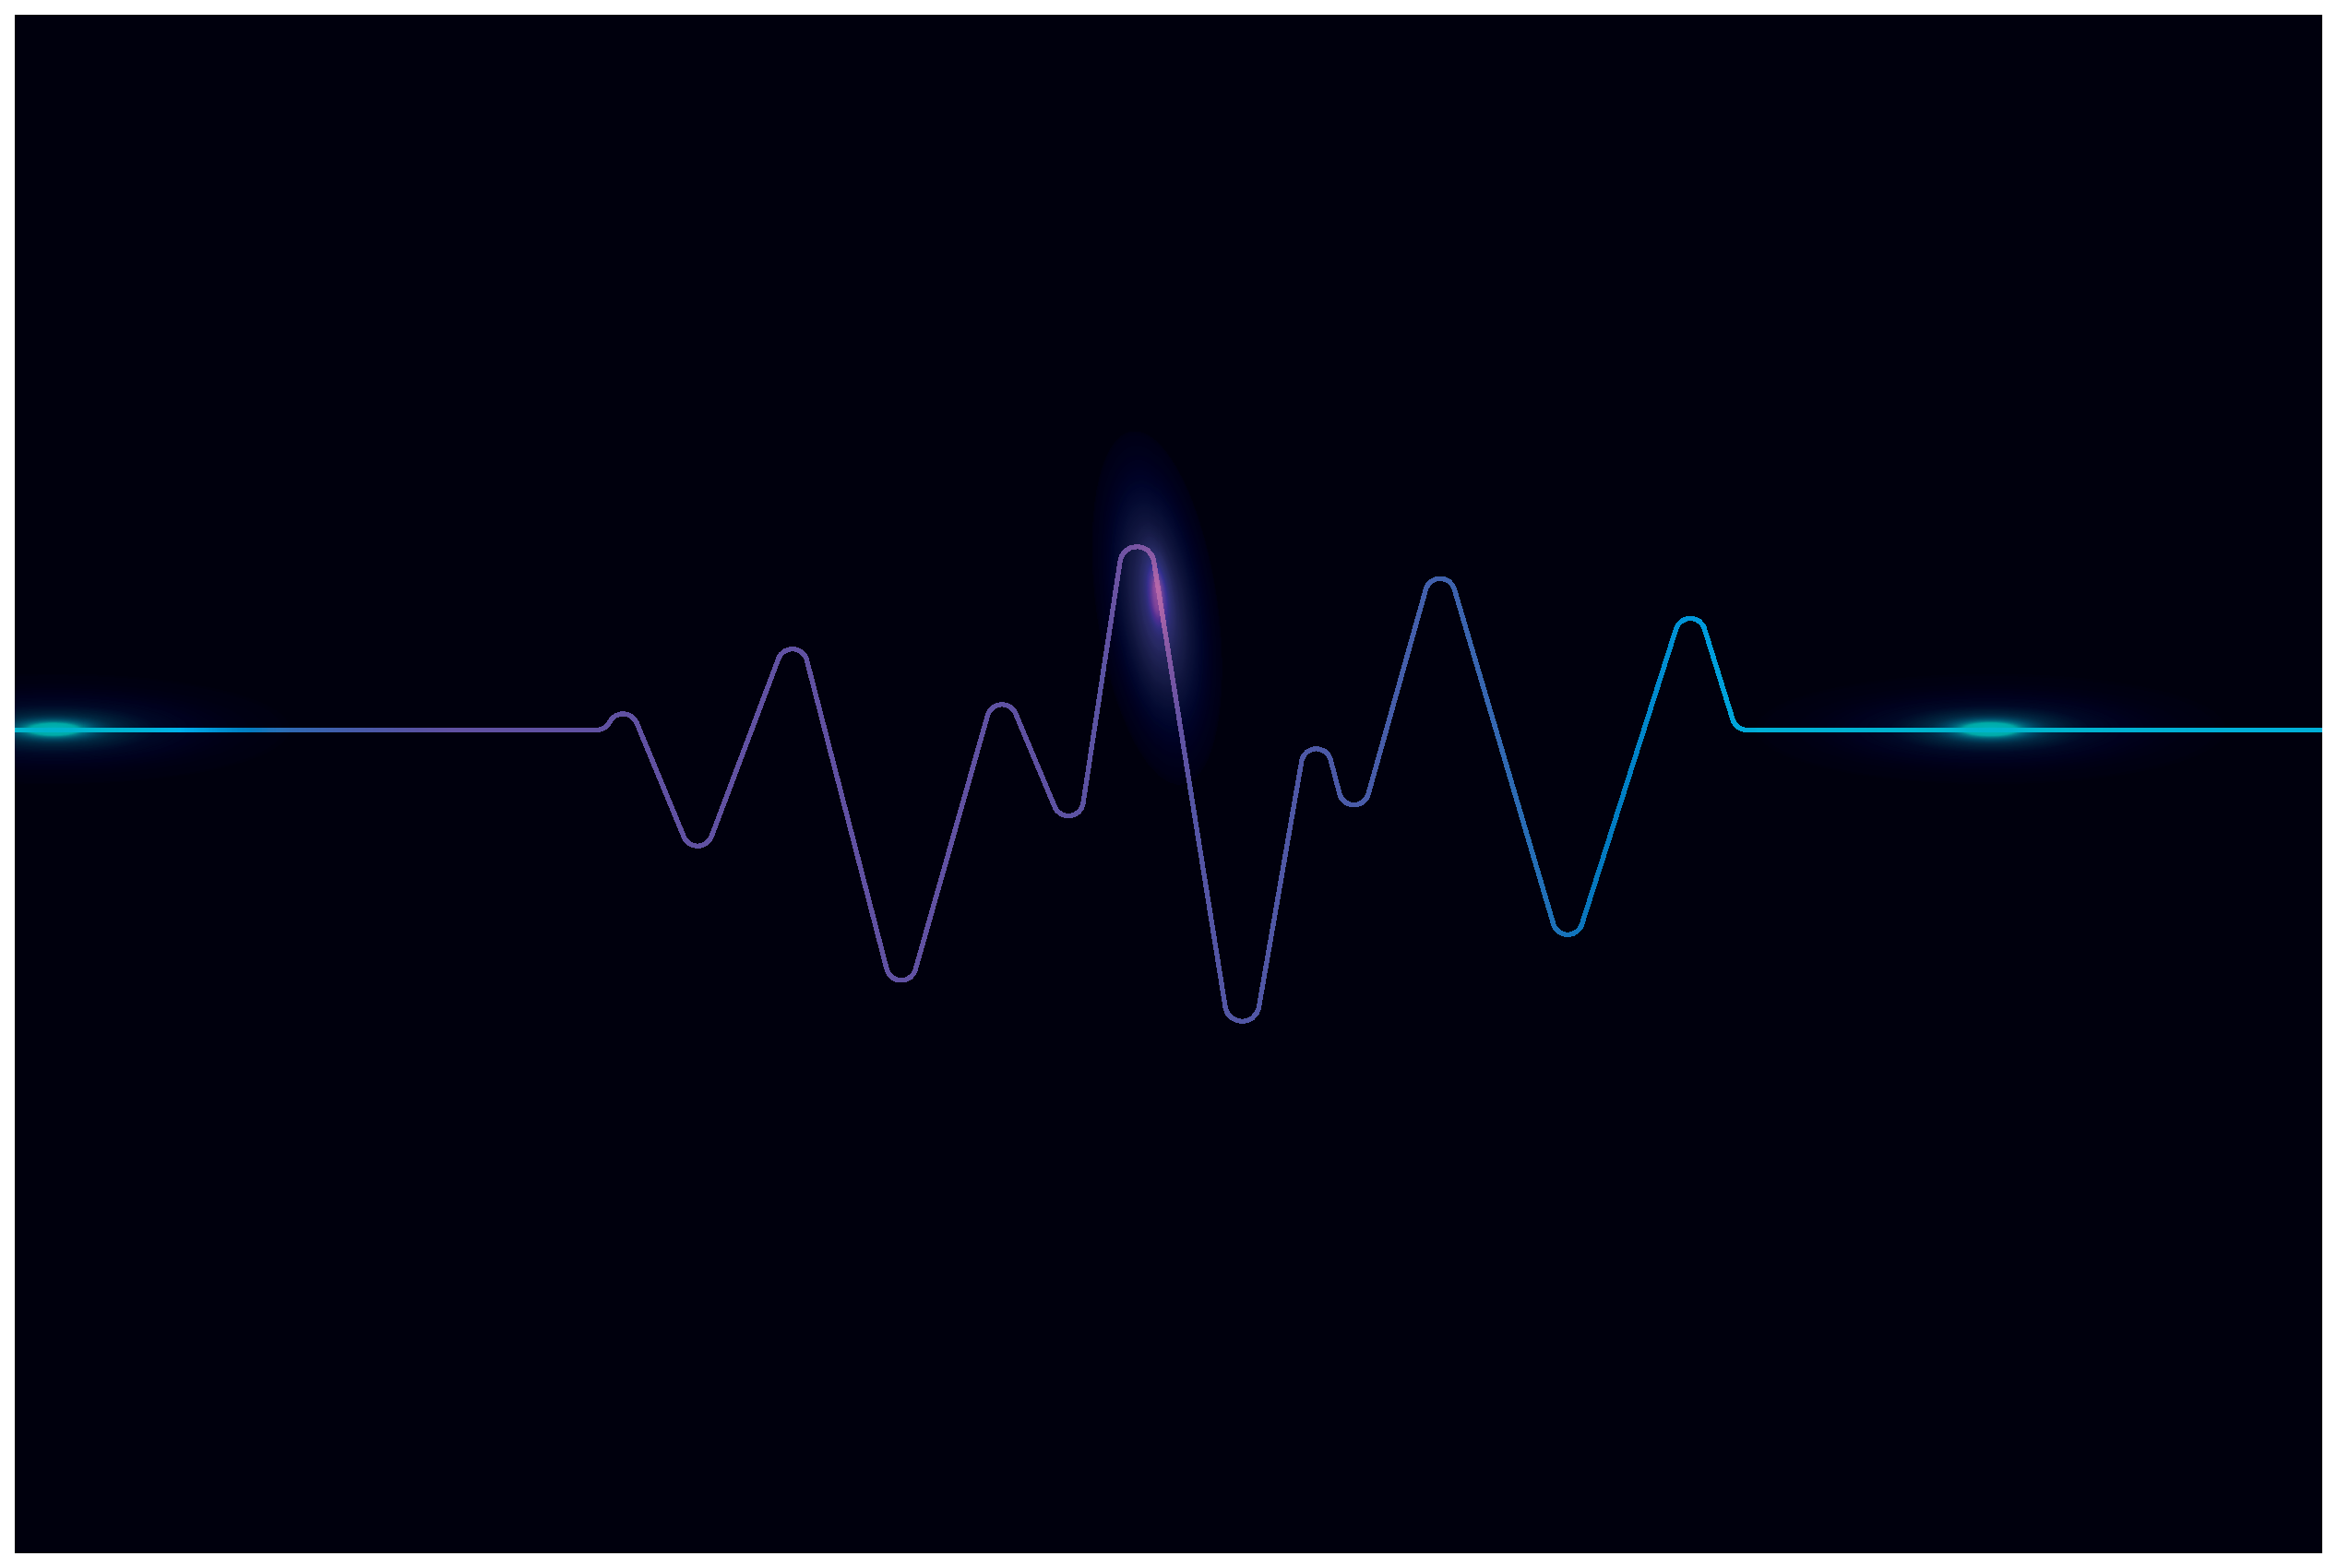
\includegraphics[height=18.9cm,keepaspectratio]{Pictures/rm383-17.eps}};
	%{\includegraphics[height=18.9cm,keepaspectratio]{Pictures/COLOURBOX54612724.eps}};
\end{tikzpicture}

%% BMM logo
%\begin{tikzpicture}[remember picture,overlay]
%	\node[anchor=north west, 
%	xshift=65mm, 
%	yshift=-11mm] 
%	at (current page.north west) 
%	{
\includegraphics[width=35.25mm,keepaspectratio]{Pictures/Logos/bmm_white.eps}}; 
%	%{\includesvg[width=44.25mm,keepaspectratio]{Pictures/Logos/bmm_white.svg}}; 
%\end{tikzpicture}


\end{titlepage}

\pagecolor{white}
\newgeometry{top=2.81cm, bottom=2.75cm, outer=2.5cm, inner=3.5cm}
\pagestyle{empty}
%\cleardoublepage 
\thispagestyle{empty}
%\setcounter{page}{1}
\vspace*{\fill}

%\begin{figure}
%	\centering
%	%\includesvg[width=0.3\textwidth]{Pictures/Logos/bmm_black.svg}
%	
\includegraphics[width=0.3\textwidth]{Pictures/Logos/bmm_black.eps}
%\end{figure}

\textbf{\thesistitle} \newline
\thesissubtitle

\smallskip

\documenttype \newline
\thedate

\smallskip

\textbf{Author:} \newline
\thesisauthor

\textbf{Advisor(s):} \newline
Hyunjoo Lee, Associate Professor, School of Electrical Engineering, KAIST \newline
Xenofon Fafoutis, Associate Professor, Department of Applied Mathematics and Computer Science, DTU \newline
Tiberiu Gabriel Zsurzsan, Associate Professor, Department of Electrical Engineering, DTU \newline

\bigskip

\begin{tabularx}{\textwidth}{@{}lX@{}}
    Copyright: & Reproduction of this publication in whole, or in part, must include the customary bibliographic citation, including author attribution, report title, etc. \\
    Cover photo: & RawPixel, 2022 \\
    Published by (1): & DTU, \dtudepartmentdescriber, \dtuaddressI, \dtuaddressII,~Denmark  \\
     & \url{\dtudepartmentwebsite} \\
    Published by (2): & KAIST, \kaistdepartmentdescriber, \kaistaddressI \kaistaddressII~대한민국 \\ & \url{\kaistdepartmentwebsite} \\
    Timespan: & \projectstartdate ~ \projectenddate \\
    Credits: & \projectcredits \\
    & \\
    Degree: & \degreetype \\
    Field: & \degreename \\
\end{tabularx}



\clearpage 
%\pagestyle{front}
%\thispagestyle{main}
%\setcounter{page}{1}

%\chapter*{Approval \markboth{Approval}{}}
\chapter*{Approval}
\addcontentsline{toc}{chapter}{Approval}
This thesis has been prepared over six months at the Brain/Biomedical Microsystems Laboratory, School of Electrical Engineering, at the Korean Advanced Institute of Science and Technology, KAIST, and the Department of Electrical Engineering, Technical University of Denmark, DTU. This thesis is in partial fulfillment for the double degree Master of Science in Electrical Engineering (M.S.E.E.) from KAIST and DTU.

\vfill

\begin{center}
\namesigdate{\thesisauthor~-~\studentnumber}
\end{center}
\thispagestyle{empty}
\vfill


%\clearpage 
%
% Multiple abstracts on the same page
\newenvironment{abstractpage}
%{\cleardoublepage\vspace*{\fill}\thispagestyle{empty}}
%{\clearpage\vspace*{\fill}\thispagestyle{empty}}
{\vspace*{\fill}\thispagestyle{empty}}
{\vfill\clearpage}
\renewenvironment{abstract}[1]
{\bigskip\selectlanguage{#1}%
	\begin{center}\bfseries\abstractname\end{center}}
{\par\bigskip}

\chapter*{Abstract}
\addcontentsline{toc}{chapter}{Abstract}

\begin{abstractpage}
	\begin{abstract}{english}
		Hello, here is some text without a meaning. This text should show what a printed text will look like at this place. If you read this text, you will get no information. Really? Is there no information? Is there a difference between this text and some nonsense like “Huardest gefburn”? Kjift – not at all! A blind text like this gives you information about the selected font, how the letters are written and an impression of the look. This text should contain all letters of the alphabet and it should be written in of the original language. There is no need for special content, but the length of words should match the language.
	\end{abstract}
	
	\begin{abstract}{danish}
		Hej, her er noget tekst uden mening. Denne tekst skal vise, hvordan en trykt tekst vil se ud på dette sted. Hvis du læser denne tekst, får du ingen information. Virkelig? Er der ingen information? Er der forskel på denne tekst og noget nonsens som "Huardest gefburn"? Kjift – slet ikke! En blindtekst som denne giver dig information om den valgte skrifttype, hvordan bogstaverne er skrevet og et indtryk af udseendet. Denne tekst skal indeholde alle bogstaver i alfabetet, og den skal være skrevet på originalsproget. Der er ikke behov for særligt indhold, men længden af ord skal passe til sproget.
	\end{abstract}
	
	\begin{abstract}{korean}
		안녕하세요, 여기 의미 없는 문자가 있습니다. 이 텍스트는 이 플레이스에서 인쇄된 텍스트의 모양을 보여줘야 합니다. 이 텍스트를 읽으면 정보를 얻을 수 없습니다. 정말? 정보가 없나요? 이 텍스트와 "Huardest gefburn"과 같은 말도 안 되는 내용 사이에 차이가 있나요? Kjift – 전혀 그렇지 않습니다! 이와 같은 블라인드 텍스트는 선택한 글꼴, 글자의 작성 방법 및 모양에 대한 정보를 제공합니다. 이 텍스트는 알파벳의 모든 문자를 포함해야 하며 원래 언어로 작성되어야 합니다. 특별한 내용은 필요 없지만, 단어의 길이는 언어와 일치해야 합니다.
	\end{abstract}
\end{abstractpage}
%\clearpage 
%%\thispagestyle{empty}
\thispagestyle{main}
\chapter*{Acknowledgements}
\addcontentsline{toc}{chapter}{Acknowledgements}
I would like to express my sincere gratitude to all those who have contributed to the completion of this thesis.

Firstly, I would like to thank my advisors, Lee Hyunjoo, Fontas, and Gabriel, for their guidance and support throughout the entire research process. Their valuable feedback and constructive criticism have been instrumental in shaping my ideas and improving the quality of my work.

I would also like to extend my gratitude to the members of Brain/Bio Medical Microsystems Laboratory, who have inspired me during my academic journey. Their kindness creates a positive atmosphere and their profound knowledge have provided me with a solid foundation for conducting research.

I am deeply grateful to my family and friends for their unwavering support and encouragement, both academically and personally. Their love, care, and motivation have kept me going during the challenging times of this project.

Finally, I would like to acknowledge the collaborative work done with Sangmok and Taemin, whose willingness to take part in this research has made it possible for me to generate meaningful findings. Their insights and experiences have been invaluable in helping me to answer my research questions.

%\cleardoublepage
\tableofcontents
\cleardoublepage
%\listoffigures
%\listoftables
%\printglossary[type=\acronymtype,title=Acronyms,toctitle=Acronyms, style=long-booktabs]
\renewcommand{\printunsrtglossaryentryprocesshook}[1]{%
    \glsifcategory{#1}{glosscat}%
    {\printunsrtglossaryskipentry}%
    {}%
}
\printglossary[type=\acronymtype,title=Acronyms,toctitle=Acronyms, style=long-booktabs]
%\printglossary[type=main, title={Glossary}, style=long-booktabs]
\renewcommand{\printunsrtglossaryentryprocesshook}[1]{%
    \glsifcategory{#1}{acronymcat}%
    {\printunsrtglossaryskipentry}%
    {}%
}
\printunsrtglossary[type=main, title={Glossary}, style=long-booktabs]
\cleardoublepage
%%%%%%%%%%%%%%%%%%%%%%%%%%%%%%%%%%%%%%%%%%%%%%%%%%%%%%%
\pagenumbering{arabic}
\pagestyle{main}
\chapter{Introduction} \label{cha:introduction} %\thispagestyle{main}
The progress of diagnostic imaging has advanced significantly during the \nth{20} century. As the cost of high-speed computational systems has grown increasingly accessible, so has the use of medical imaging become prominent. Millions of people have potentially been spared painful exploratory surgery through non-invasive diagnostic imaging. Thus, lives can be saved by early diagnosis and intervention through medical imaging. Advancements in scientific visualisation have in turn generated more complex data-sets of increased size and quality. The four major technologies used are \gls{us}, X-ray, \gls{ct}, and \gls{mri}. Each technology has distinct advantages and disadvantages in biomedical imaging, and thus each is still relevant for modern medicine. \Cref{tab:1_imagingmodalities} contains a comparison and summary of the various fundamental diagnostic imaging modalities.

\begin{table}[htbp]
	\centering
	\begin{talltblr}[
	caption = {Comparison of medical imaging modalities \cite{Szabo_UltrasoundBook_2}},
	entry = {Comparison of medical imaging modalities},
	label = {tab:1_imagingmodalities},
	note{a} = {Frequency and axially dependent.},
	note{b} = {Frequency dependent.},
	note{c} = {Fluoroscopy limited.},
	note{$\dag$} = {Typical: 45 minutes, fastest: Real-time (\glsxtrshort{low-res}).},
	]{
		%colspec = {Q[l,t]Q[l,t]Q[l,t]Q[l,t]Q[l,t]},
		%colspec = {Q[jQQQQ},
		row{1} = {guard, m, font=\small\bfseries},
	}
	\toprule
	\textbf{Modality} & \textbf{Ultrasound} & \textbf{X-ray} & \textbf{CT} & \textbf{MRI} \\ \midrule
	Topic             & {Longitudinal,\\shear,\\mechanical\\properties} & {Mean X-ray\\tissue\\absorption} & {Local tissue\\X-ray absorbtion} & {Biochemistry \\(\textit{T1} and \textit{T2})}    \\
	Access            & {Small\\windows\\adequate} & {2 sides\\needed} & {Circumferential\\around\\body} & {Circumferential\\around\\body} \\
	{Spatial\\resolution} & {\qty{0.2}{\milli\meter} to\\\qty{3}{\milli\meter}\TblrNote{a}} & $\sim \qty{1}{\milli \meter}$ & $\sim \qty{1}{\milli \meter}$ & $\sim \qty{1}{\milli \meter}$ \\
	Penetration     & {\qty{3}{\centi\meter} to\\\qty{25}{\centi\meter}\TblrNote{b}} & Excellent  & Excellent & Excellent \\
	Safety          & Excellent & {Ionizing\\radiation}      & {Ionizing\\radiation} & Very good \\
	Speed           & Real-time & Minutes & 20 minutes & Varies\TblrNote{$\dag$} \\
	Cost            & \$ & \$ & \$\$ & \$\$\$ \\
	Portability     & Excellent & Good & Poor & Poor \\
	{Volume\\coverage} & {Real-time\\3D volumes,\\improving} & 2D & {Large 3D\\volume} & {Large 3D \\volume} \\
	Contrast        & {Increasing\\(shear)} & Limited & Limited & {Slightly\\flexible} \\
	Intervention    & {Real-time\\3D increasing} & No\TblrNote{c} & No & Yes, limited \\
	Functional      & {Functional\\ultrasound} & No & No & fMRI \\
	\bottomrule
\end{talltblr}
\end{table}

Between 2004 and 2016\todo{Fix end year}, medical imaging has been reported to have been performed more than 5 billion times \cite{Picano2004}. Later numbers from 2011 show a general doubling and in particular, a tenfold increase in ultrasound examinations between 2000 and 2011 \cite{Szabo_UltrasoundBook_2}. Recent data reveal that this trend of doubling has continued throughout the years 2010 to 2020 \cite{Winder2021}, and reveal that even though patient processes were disrupted during the global SARS-CoV-2 pandemic, the number of medical imaging examinations per 1000 patients still increased. The reasons for this and, particularly, why ultrasound has seen a significant increase in use, can be attributed to its high resolution, cost-effectiveness, portability, and real-time interventional imaging. The downside of ultrasound is its limited penetration, restrictions for use in certain body parts, and inconsistent resolution. When comparing soft tissue examinations, which ultrasound is limited to, both \gls{ct} and \gls{mri} can image the entire body with consistent resolution and contrast, but are more expensive and have poor portability due to the immense size of their hardware.

The cardiovascular system, which transports oxygen and nutrients to tissue, produces a complex flow pattern that causes velocity fluctuations. Several \gls{cvd} are also known to cause abnormal blood flow. In studies published by the Centers for Disease Control, a person dies from CVD every 34 seconds in the United States and complications from CVD cost 229 billion USD between 2017 and 2018 \cite{cdc_2022}. As mentioned above, ultrasound is a powerful tool for performing non-invasive imaging of the cardiovascular system \cite{JensenUltrasoundBook,Hansen_thesis}, and has no adverse risk to patients. Determining \gls{psd} of a received signal is a common way to estimate blood velocity. A processed image of \gls{psd} over time is commonly known as a sonogram, where changes in blood velocity over time can be seen.\todo{Check over-time repetitive}

\section{Literature review}
%The aim of this project is to study the application of ultrasound in the context of blood flow measurements. Various scientific articles have been studied to gain knowledge of previous research \cite{Jensen_Analysis_PW_1996,Jansson_Estimation_Perfusion,Huang_Smartphone_2012,JanaSmartphone2020,DingPMUTs,Ding_PW_Pmut,Xu2007_Pulser,Matsuoka_Doppler_Rabbit,Fish_Ultrasonic,Williams2006,Winckler2012,Wang2016,Wang2019,Tsang2009,Govindan2016,Xu2007_Pulser,PICpulser}. In addition, textbooks \cite{JensenUltrasoundBook,ShungUltrasound_Book,Szabo_UltrasoundBook_2} have also been instrumental in forming a solid knowledge base for the thesis.

%The delimitation of this work is done through a literature review in the field of blood flow estimation using ultrasound. One of the earliest concepts for a device to estimate and study blood flow using ultrasound was developed during the 1950s in Japan and published internationally by \cite{Satomura_CW}. In this journal article, \citeauthor{Satomura_CW} study the valvular movements using echocardiography and made several important discoveries on the distinctions in myocardial change between healthy patients and patients suffering from \gls{cvd}. Articles such as \cite{Jensen_Analysis_PW_1996,Wells1998,PWDesignParameters,Jansson_Estimation_Perfusion,PWDesignParameters} outline the Doppler ultrasound analysis.
A systematic review was conducted using PubMed, Google Scholar, Elsevier, DTU FindIt and IEEE Xplore with the search terms \enquote{pulsed-wave Doppler ultrasound}, \enquote{blood velocity estimation}, and \enquote{ultrasound flow-meter}. The search was limited to English-language articles. The literature search yielded more than 50 papers, of which 37 were studied for the purpose of learning from the contents \cite{Satomura_CW,Baker1970,Shung1976,Schlindwein1988,Hall_Wall_Filter,Jensen_Analysis_PW_1996,Wells1998,PWDesignParameters,Jansson_Estimation_Perfusion,Hoskins_Review_Blood_Velocity,Fish_Ultrasonic,Jensen_Algorithms,cmut_array_shape,Williams2006,Tsang2009,Matsuoka_Doppler_Rabbit,Hoskins2010,PICpulser,Advances_BloodFlow_Velocity,Overview_Emerging_Imaging,Huang_Smartphone_2012,DesignDocument,Winckler2012,Sagdiev2014,Jacinta_string_phantom,500Vpulser,Wang2016,Govindan2016,Wang2019,JanaSmartphone2020,Ding_PW_Pmut,DingPMUTs,Winder2021,Omura2022,2023_review,Ricci2018,Bessi1995}. In addition, textbooks \cite{JensenUltrasoundBook,ShungUltrasound_Book,Szabo_UltrasoundBook_2} were used in the preparation and study of the theoretical principles of biomedical imaging and ultrasound.

Among these works are some of the earliest papers that outlined the field as it was emerging. Other articles study the possibilities of improvements in algorithms and experimental parameters. Overall, the results indicate that the Doppler flow meter is a reliable method for estimating blood flow velocity in various parts of the body. Studies include experiments using physiological simulators and in-vivo on humans and animals alike. Some of the review articles have compared Doppler flow-meters to other imaging techniques for this application, such as magnetic resonance imaging and computed tomography angiography, and have shown that the Doppler flow-meter is a cost-effective, portable and non-invasive choice.
%
%\begin{table}[htbp]
%	\centering
%	\begin{adjustbox}{max width=\textwidth}
%	\begin{talltblr}[
%		caption={Comparison of papers in literature study},
%		entry={Comparison of papers in literature study},
%		label={tab:1_papercomparison}]{
%			row{1} = {guard, m, font=\small\bfseries},
%		}
%		\toprule
%		Author & Architecture & Type & Power & System Components & DSP & Metrics & Output & Validation \\
%		\midrule
%		\citeauthor{Huang_Smartphone_2012} \cite{Huang_Smartphone_2012} & {\gls{pw},\\\qty{10}{\mega\hertz}} & Smartphone & \qty{12}{\volt} & {\gls{prf} timer, bipolar\\pulser, quadrature\\demodulation, \gls{sha}} & 512 point \gls{fft} & Doppler spectrogram & Microphone auxiliary signal to smartphone & In-vivo animal experiment \\
%		\citeauthor{JanaSmartphone2020} \cite{JanaSmartphone2020} & {\gls{cw},\\\qty{8}{\mega\hertz}} & {Portable\\device} & \qty{12}{\volt} & \gls{rf} amplifier, envelope detection, \gls{lp} filter, preamplifier, \gls{adc} & 512 point \gls{fft} & \gls{ml} performance estimator on humans \\
%		\citeauthor{DingPMUTs} \cite{DingPMUTs} & {\gls{pw},\\\qty{3.7}{\mega\hertz}} & Smartphone & {Details not\\available} & {Function generator, \gls{rf}\\amplifier, quadrature demodulation,\\\gls{sha}, \gls{bp} filter,\\\gls{daq} module, LabVIEW} & {\gls{fft} size\\not mentioned} & {Physiological simulation\\using blood mimicking fluid\\in pumped tubing system} \\
%		\bottomrule
%	\end{talltblr}
%	\end{adjustbox}%
%\end{table}

\begin{table}
	\centering
	\begin{adjustbox}{max width=\textwidth}
		\begin{talltblr}[
			caption={Comparison of papers in literature study},
			entry={Comparison of papers in literature study},
			label={tab:1_papercomparison}]{
				row{1} = {guard, m, font=\small\bfseries},
			}
			\toprule
			& \citeauthor{Huang_Smartphone_2012} \cite{Huang_Smartphone_2012} & \citeauthor{JanaSmartphone2020} \cite{JanaSmartphone2020} & \citeauthor{DingPMUTs} \cite{DingPMUTs} \\
			\midrule
			Architecture & {PW \qty{10}{\mega\hertz}} & {CW \qty{8}{\mega\hertz}} & {PW \qty{3.7}{\mega\hertz}} \\
			Type & Smartphone & Portable device & Computer \\
			Power & 12 V & 12 V & Details not available \\
			Components & {PRF timer,\\bipolar pulser,\\quadrature demodulation,\\SHA} & {RF amplifier,\\envelope detection,\\LP filter, FPGA,\\preamplifier, ADC} & {AFG, RF amplifier,\\quadrature demodulation,\\SHA, BP filter}\\
			DSP & 512 pt FFT & 512 pt FFT & FFT size not mentioned \\
			Metrics & Doppler spectrogram & Haemodynamic parameters & Doppler spectrogram \\
			Output & Aux microphone signal & Bluetooth & {DAQ input signal \\ (LabVIEW)} \\
			Validation & In-vivo animal experiment & ML evaluation on humans & Physiological simulator \\
			\bottomrule
		\end{talltblr}
	\end{adjustbox}%
\end{table}
Of the selected papers studied in this project, three papers are distinctly relevant for the design and implementation of a blood velocity estimation system. A comparison between these three papers can be seen in \cref{tab:1_papercomparison}. Based on the literature review, a gap is identified in the acquisition method of the signal chain. A number of articles studied and developed the algorithms for blood flow estimation and imaging, but do did have an \gls{afe} and used offline data acquisition methods which are not usable for clinicians. The selected three articles all feature an online data acquisition method using various methods of data capture. There is a potential to using selected features from all three articles in a combination to achieve a positive result. For instance, the \gls{afe} in \citeauthor{Huang_Smartphone_2012} is better documented than both other papers, and feature a \gls{pw} design that could be useful. On the other hand, their solution for the pulser is dated and use inflexible discrete timer \gls{ic}s. \citeauthor{JanaSmartphone2020} use a \gls{cw} based design and thus most details are on the receiver. However, it features an \gls{fpga} \gls{soft microprocessor} design to the \gls{fft} engine. \citeauthor{DingPMUTs} feature a \gls{pw} design, and use an \gls{afg} as the primary signal generator for the pulser as well as the demodulation clock. In that paper, there are some good figures for studying the pulse-echo waveforms of the \gls{pw} type system.

Some of the project decisions resulting out of the study of these three papers include the desire to implement an \gls{afe} for a pulsed-wave system using the inspiration from all three papers, but also implement a novel pulse generator not using discrete \gls{ic}s or with a lab instrument \gls{afg}, since it is not portable. Instead, with a flexible and configurable design that an embedded system enables.

\section{Project scope}
%The desire is to build upon the vast knowledge already gathered by prominent researchers in the field of ultrasound systems for blood velocity estimation. Finally, using the knowledge gained, we designed and implemented an electronic device capable of performing these measurements using a novel approach. The system used in this project is called an Ultrasound Doppler flow-meter. Ultrasound Doppler flow-meters can be used to measure the velocity of blood flow in the human body. This is commonly done to assess the health of blood vessels and to diagnose and monitor conditions such as arteriosclerosis (hardening of the arteries) and deep vein thrombosis (blood clots in the veins). To measure blood velocity with an ultrasound Doppler flow-meter, a handheld probe is placed on the skin over the area of interest, such as an artery or vein. The probe contains a transducer that emits high-frequency ultrasound waves and receives the reflected waves. The Doppler shift in the frequency of the reflected waves is caused by the movement of the blood cells, and it is proportional to the velocity of the blood flow. The probe is connected to a portable ultrasound machine, which processes the Doppler shift and displays the velocity of the blood flow on a screen. The machine can also produce a color-coded map of the blood flow, which allows the user to visualize the velocity of the blood at different points within the vessel. Ultrasound Doppler flow-meters are non-invasive and safe to use, and they provide a quick and easy way to measure blood velocity. However, they are not always accurate, especially in cases where there is a high degree of turbulence or when there are air bubbles or solid particles present in the blood. They are also limited in their ability to measure blood flow in small vessels or in deep tissues. The goals of the project are written in \cref{tab:specifications}.

\begin{table}[htbp]
	\centering
	\caption{Project specification}
	\label{tab:specifications}
	\begin{tblr}[]{%
			%width=.9\textwidth,
			colspec = {l
			},
			row{1} = {guard, m, font=\small\bfseries},
			%vlines, hlines,
		}
		\toprule
		Project specification	\\
		\midrule
		Study and research ultrasound and its principles and applications	\\
		Design and implement a device for ultrasound blood velocity estimation	\\
		Investigate and test the device in an experimental setting		\\
		Validate results with commercial equipment 						\\
		Make quantifiable performance measurements on the system			\\
		Write a technical report documenting the project work			\\ \bottomrule
	\end{tblr}
\end{table}

A list of project goals is provided in \cref{tab:specifications}. The project is conducted under the guidance of advisors from the affiliated institutions \Gls{dtu}, Department of Electrical Engineering, Department of Applied Mathematics and Computer Science, and \Gls{kaist} at the Brain/Bio Medical Microsystems Laboratory. \todo{Omskriv til lab før uni} The report is divided into five chapters, and the first part is an introduction to the project. The second chapter will focus on explaining the theory of the topic of the project. The third chapter focuses on the synthesis of a system model for experimental testing. The fourth chapter explains the method of implementation during the assembly of the system. The fifth chapter will explain the testing methodology performed on the hardware. Finally, additional documentation of testing, code, circuit diagrams, and laboratory setups can be found in the appendix.

\begin{ganttchart}[%Specs
	y unit title=0.5cm,
	y unit chart=0.5cm,
	vgrid,
	title height=1,
	title/.style={fill=lightgray},
	title label font=\bfseries\footnotesize,
	bar/.style={fill=cyan},
	bar height=0.7,
	%   progress label text={},
	group right shift=0,
	group top shift=0.7,
	group height=.3,
	group peaks width={0.2},
	inline]{1}{8}
	%labels
	\gantttitle{M.S. Thesis Research Schedule}{12}\\  % title 1
	%			\gantttitle[]{2021}{6}                 % title 2
	\gantttitle[]{2022}{3}
	\gantttitle[]{2023}{6} \\
	%			\gantttitle{Q3}{3}
	%			\gantttitle{Q4}{3}
	%			\gantttitle{Q1}{3}
	%			\gantttitle{Q2}{3}
%	\gantttitle{7}{1}
%	\gantttitle{8}{1}
%	\gantttitle{9}{1}
	\gantttitle{10}{1}
	\gantttitle{11}{1}
	\gantttitle{12}{1}
	\gantttitle{1}{1}
	\gantttitle{2}{1}
	\gantttitle{3}{1}
	\gantttitle{4}{1}
	\gantttitle{5}{1}
	\gantttitle{6}{1} \\
	%			\gantttitle{Q3}{3}
	%			\gantttitle{Q4}{3}
	%			\gantttitle{Q1}{3}
	%\gantttitle{Q2}{3} \\
	% Setting group if any
	%			\ganttgroup[inline=false]{Phase 1 (Basic Research)}{1}{6}\\
	%			\ganttbar[inline=false]{Study}{1}{3} \\
	%			\ganttbar[inline=false]{Laboratory experiments}{2}{4} \ganttbar[inline=false]{Laboratory experiments}{6}{6} \\
	%			\ganttbar[inline=false]{Initial PCB design}{2}{5}\\
	%			\ganttmilestone[inline=false]{End-of-Year 2021 Milestone}{6} \\

	\ganttgroup[inline=false]{Circuit and experiments}{4}{10} \\
	\ganttbar[progress=0,progress label text={},inline=false]{PCB integration layout}{4}{6} \\
	\ganttbar[progress=0,progress label text={},inline=false, bar progress label node/.append style={below left= 10pt and 7pt}]{Auxiliary circuitry design}{5}{7} \\
	\ganttbar[progress=0,progress label text={},inline=false]{Testing}{6}{10}\\

	\ganttgroup[inline=false]{Embedded}{2}{6} \\
	\ganttbar[progress=100,inline=false, progress label text={}]{Ultrasound pulser}{2}{5} \\
	\ganttbar[progress=25,progress label text={},inline=false]{Data processing}{3}{6} \\
	%			\ganttmilestone[inline=false]{Applied Study Completed Milestone}{3} \\
	\ganttbar[progress=0,progress label text={},inline=false]{Writing thesis report}{3}{10}\\
	\ganttmilestone[inline=false]{Deadline}{9}
\end{ganttchart}
\cleardoublepage
\chapter{Colours} \label{sec:colours}
The design guide define 3 primary colours (dtured, white and black) and 10 secondary colours \url{https://www.designguide.dtu.dk/#stnd-colours}. Below are codes for the various colour modes. RGB is used for web and Office Programmes. CMYK is used for print. HTML is used for HTML-coding. If you know anything about colour codes you might notice that the RGB codes are ranging from 0-1 instead of the usual 0-255. 

\begin{testcolors}[rgb,cmyk,HTML]
\testcolor{dtured}
\testcolor{white}
\testcolor{black}
\testcolor{blue}
\testcolor{brightgreen}
\testcolor{navyblue}
\testcolor{yellow}
\testcolor{orange}
\testcolor{pink}
\testcolor{red}
\testcolor{green}
\testcolor{purple}
\end{testcolors}

The default colour mode for this template is cmyk. The current colour model is \targetcolourmodel~which is also illustrated by the underlined numbers in the colour test table above.  If you which to change the colour model to rgb go to Setup/Settings.tex and change \texttt{targetcolourmodel} to rgb. In Setup/Settings.tex it is also possible to change the background colour of the front and back page. The colours are primarily used for diagrams (the plotcyclelist DTU) and the front and back page.

Lighter colours can be achieved as written in the \LaTeX{} code below. For example to get a tint of 50\% you would write colourname!50.  \newline
{\raggedright
\textcolor{dtured}{Normal dtured} \qquad
\textcolor{dtured!80}{80\% dtured} \qquad 
\textcolor{dtured!70}{70\% dtured} \qquad
\textcolor{dtured!60}{60\% dtured} \qquad
\textcolor{dtured!50}{50\% dtured} 
}
\newline
For more information about colours in \LaTeX{} read the \texttt{xcolor} manual. I want to use the MCU \cite{f411re} for the \glsxtrshort{mcu} part of the project. \gls{mcu}
\cleardoublepage
\chapter{Examples of figures, tables, equations and listings}
In the following a bunch of examples of figures and tables have been made. There are advantages to using \texttt{tikZ} diagrams over excel diagrams. 1) the font and font size perfectly matches the document 2) the styling and colours are pre-defined to follow the design guide 3) the plots uses vector graphics which reduces the file size, reduces the compile time and looks sharp when zooming in. The possibilities are endless, look at the \texttt{pgfplots} gallery for inspiration: \url{http://pgfplots.sourceforge.net/gallery.html}. 
However there are still cases where I would recommend to insert a plot as a picture. For example if the plot contains a lot of data: a line graph with 1000 points takes a long time to compile. 

Some tips if you want good looking diagrams or graphs which will be inserted as pictures (e.g. in a figure environment with \textbackslash includegraphics): The main font is Arial. Use DTU colours as described in \cref{sec:colours}. Use high quality pictures. Try to scale the diagram (picture) so the text size of the axis legends match the text size in this document.

Remember to change the label of your figures so there are no duplicate labels. A label should be placed below a caption or after a heading (fx after a \textbackslash chapter). 





\section{Graphs and charts}

\pgfplotstableread{
x  {Name 1} {Name 2}    {Name 3}    {Name 4}
1  0.847    0.786       0.367       0.742
2  1.73     0.838       1.27        1.05
3  1.50     0.952       0           0
4  0.506    1.05        0.751       0.698
5  0.672    0.777       0           0
6  0.349    1.62        1.16        0.655
7  0.498    0.480       0.375       0.306
8  0.454    0.925       0.498       0.375
9  0.698    0.716       0.733       0.541
10 0.829    1.12        0.803       0.725
}\stackedColumnData

\begin{figure}[htb]
\centering
\begin{tikzpicture} 
\begin{axis}[ 
    width=15cm, % You could use \linewidth instead 
    height=6.6cm,
    ybar stacked, 
    xtick = data,
    xticklabels={1,2,3,4,5,6,Var 1,Var 2,Var 3,Var 4},
    ylabel={Some text with a unit $\phi$ }, 
    ymajorgrids=true,
    legend style={at={(0.5,-0.1)}, anchor=north}, 
    cycle list name=DTU,
    every axis plot/.append style={fill,draw=none},
    ] 
\addplot table[x=x,y={Name 1}]{\stackedColumnData}; 
\addplot table[x=x,y={Name 2}]{\stackedColumnData};
\addplot table[x=x,y={Name 3}]{\stackedColumnData};
\addplot table[x=x,y={Name 4}]{\stackedColumnData};
\legend{Heating,Ventilation,Lighting,Solar shading} 
\end{axis} 
\end{tikzpicture}
\caption{Stacked column chart}
\label{fig:stackedcolumn}
\end{figure}



\pgfplotstableread{
y {Name 1} {Name 2} {Name 3} {Name 4} 
1 50        20      15       15
2 10        40      25       25
3 40        30      20       10
4 30        10      20       40
5 30        20      10       40
6 20        10      40       30
7 10        10      50       30
}\stackedBarData

\begin{figure}[H]%
\centering
\begin{tikzpicture}
\begin{axis}[
    width=15cm-10pt, % pgfplots widths are only approximate. You might have to fine tune the width of your figures to deal with overfull hbox warnings. 
    height = 6.6cm,
    xbar stacked,
    xlabel=Write something here,
    ytick=data,
    yticklabels = {Text 1, Text 2, Text 3, Text 4, Text 5, Text 6, Text 7},
    xmin = 0,
    enlarge x limits=false,
    xmajorgrids=true,
    legend style={at={(0.5,-0.22)}},
    cycle list name=DTU,
    every axis plot/.append style={fill,draw=none},
    ]
\addplot table[x={Name 1},y=y]{\stackedBarData};
\addplot table[x={Name 2},y=y]{\stackedBarData};
\addplot table[x={Name 3},y=y]{\stackedBarData};
\addplot table[x={Name 4},y=y]{\stackedBarData};
\legend{Legend 1, Legend 2, Legend 3, Legend 4} 
\end{axis}  
\end{tikzpicture}
\caption{Stacked bar chart}
\label{fig:stackedbar}
\end{figure}



\pgfplotstableread{
x    {Far}  {Near}  {Here}
1930 50     38      15
1940 33     42      12
1950 40     43      13
1960 50     45      25
1970 70     65      35
}\groupedColumnData

\begin{figure}[H]
\centering
\begin{tikzpicture} 
\begin{axis}[ 
    width=15cm,
    height=6.6cm,
    ybar,
    xtick=data,
    x tick label style={ /pgf/number format/1000 sep=}, 
    ylabel=Population,  
    ymin=0,
    ymajorgrids=true,
    legend style={at={(0.5,-0.15)},anchor=north,legend columns=-1},
    cycle list name=DTU, 
    ] 
\addplot table[x=x,y={Far}]{\groupedColumnData}; 
\addplot table[x=x,y={Near}]{\groupedColumnData};
\addplot table[x=x,y={Here}]{\groupedColumnData}; 
\addplot[red,sharp plot,update limits=false] coordinates {(1910,43) (1990,43)} node[above] at (axis cs:1950,43) {Houses}; 
\legend{Far,Near,Here,Annot} 
\end{axis} 
\end{tikzpicture}
\caption{Grouped column chart}
\label{fig:groupedcolumn}
\end{figure}



\pgfplotstableread{
x {Name 1} {Name 2} {Name 3} {Name 4} 
1 0         10       58       10
2 30        20       48       40
3 10        60       45       10.5
4 50        18       55       60
5 40        30       8        20
}\lineGraphData

\begin{figure}[H]
\centering
\begin{tikzpicture}[spy using outlines = {circle, size=2cm, magnification=5, connect spies}]
\begin{axis}[
    width=15cm,
    height=6.6cm,
    ylabel = {Unit},
    ymin = 0,
    enlarge x limits = false,
    ymajorgrids = true,
    legend style = {at={(0.5,-0.1)}, anchor=north},
    cycle list name=DTU,
    every axis plot/.append style={fill opacity=0},
    ] 
\addplot table[x=x,y={Name 1}]{\lineGraphData}; 
\addplot table[x=x,y={Name 2}]{\lineGraphData};
\addplot table[x=x,y={Name 3}]{\lineGraphData}; 
\addplot table[x=x,y={Name 4}]{\lineGraphData}; 
\legend{Legend 1, Legend 2, Legend 3, Legend 4} 
\end{axis} 
\end{tikzpicture}
\caption{Line graph}
\label{fig:linegraph}
\end{figure}



\pgfplotstableread{
x {Name 1} {Name 2} {Name 3} {Name 4} 
1 0         10       58       10
2 30        20       48       40
3 10        60       45       10.5
4 50        18       55       60
5 40        30       8        20
}\lineGraphMagnifyData

\begin{figure}[H]
\centering
\begin{tikzpicture}[spy using outlines = {circle, size=2cm, magnification=5, connect spies}]
\begin{axis}[
    width=15cm,
    height=6.6cm,
    ylabel = {Unit},
    ymin = 0,
    enlarge x limits = false,
    ymajorgrids = true,
    legend style = {at={(0.5,-0.1)}, anchor=north},
    cycle list name=DTU,
    every axis plot/.append style={fill opacity=0},
    ] 
\addplot table[x=x,y={Name 1}]{\lineGraphMagnifyData}; 
\addplot table[x=x,y={Name 2}]{\lineGraphMagnifyData};
\addplot table[x=x,y={Name 3}]{\lineGraphMagnifyData}; 
\addplot table[x=x,y={Name 4}]{\lineGraphMagnifyData}; 

\coordinate (spypoint) at (axis cs:3,10.5); % Delete this line to remove magnifying glass
\coordinate (magnifyglass) at (axis cs:3.6,12); % Delete this line to remove magnifying glass
\legend{Legend 1, Legend 2, Legend 3, Legend 4} 
\end{axis} 

\spy [black, size=2cm] on (spypoint) in node[fill=white] at (magnifyglass); % Delete this line to remove magnifying glass
\end{tikzpicture}
\caption{Line graph with magnifying glass}
\label{fig:linegraphmagnify}
\end{figure}



\pgfplotstableread{
x {Name 1} {Name 2} {Name 3} {Name 4} 
1 30        10       2        10
2 20        20       5        5
3 25        20       5        8
4 15        20       5        5
5 30        10       8        2
}\areaGraphData

\begin{figure}[H]
\centering
\begin{tikzpicture} 
\begin{axis}[
    width=15cm,
    height=6.6cm,
    stack plots=y, 
    area style,
    ylabel = {Unit},
    ymin = 0,
    enlarge x limits=false,
    ymajorgrids=true,
    legend style={at={(0.5,-0.1)}, anchor=north}, 
    cycle list name=DTU,
    ] 
\addplot table[x=x,y={Name 1}]{\areaGraphData}\closedcycle; 
\addplot table[x=x,y={Name 2}]{\areaGraphData}\closedcycle;
\addplot table[x=x,y={Name 3}]{\areaGraphData}\closedcycle; 
\addplot table[x=x,y={Name 4}]{\areaGraphData}\closedcycle; 
\legend{Legend 1, Legend 2, Legend 3, Legend 4} 
\end{axis} 
\end{tikzpicture}
\caption{Area graph}
\label{fig:areagraph}
\end{figure}



\pgfplotstableread{
x {Name 1} {Name 2} {Name 3} {Name 4} 
1   11	15	38	41
2   33	22	25	31
3   22	25	11	21
4   44	14	17	51
5   13	42	25	33
6   14	52	36	34
}\scatterData

\begin{figure}[H]
\centering
\begin{tikzpicture}
\begin{axis}[
    %enlarge x limits=true,
    ylabel = {Unit},
    ymin = 0,
    ymajorgrids=true,
    cycle list name=DTU,
]
\addplot+[only marks,mark=*]        table[x=x,y={Name 1}]{\scatterData};
\addplot+[only marks,mark=square*]  table[x=x,y={Name 2}]{\scatterData};
\addplot+[only marks,mark=triangle*]table[x=x,y={Name 3}]{\scatterData};
\addplot+[only marks,mark=+]        table[x=x,y={Name 4}]{\scatterData};
\legend{Legend 1, Legend 2, Legend 3, Legend 4} 
\end{axis}
\end{tikzpicture}
\caption{Scatter plot}
\label{fig:scatter}
\end{figure}


\begin{figure}[H]
\centering
\begin{tikzpicture}
\begin{axis}[
    boxplot/draw direction=y,
    xtick={1,2,3},
    xticklabels={Group A, Group B, Group C},
    x axis line style={opacity=0},
    enlarge y limits,
    ymajorgrids,
    cycle list name=DTU,
    every axis plot/.append style={semithick},
]
\addplot+[draw=black,
boxplot prepared={
lower whisker=42, lower quartile=45,
median=47,
upper quartile=47.5, upper whisker=48,
},
] coordinates {(0,40) (0,34) (0,56)};
\addplot+[draw=black,
boxplot prepared={
lower whisker=36, lower quartile=39,
median=40,
upper quartile=41, upper whisker=43,
},
] coordinates {};
\addplot+[draw=black,
boxplot prepared={
lower whisker=41, lower quartile=44,
median=45,
upper quartile=46, upper whisker=47,
},
] coordinates {(0,35) (0,55)};
\end{axis}
\end{tikzpicture}
\caption{Boxplot}
\label{fig:boxplot}
\end{figure}

\begin{figure}[H]
	\centering
	\begin{circuitikz}[american voltages]
		\draw
		(0,0) to [short, *-] (6,0)
		to [V, l_=$\mathrm{j}{\omega}_m \underline{\psi}^s_R$] (6,2) 
		to [R, l_=$R_R$] (6,4) 
		to [short, i_=$\underline{i}^s_R$] (5,4) 
		(0,0) to [open, v^>=$\underline{u}^s_s$] (0,4) 
		to [short, *- ,i=$\underline{i}^s_s$] (1,4) 
		to [R, l=$R_s$] (3,4)
		to [L, l=$L_{\sigma}$] (5,4) 
		to [short, i_=$\underline{i}^s_M$] (5,3) 
		to [L, l_=$L_M$] (5,0); 
	\end{circuitikz}
	\caption{The nodes short, V, R and L are presented here, but there a lot more}
	\label{fig:circuitikz}
\end{figure}




\section{Tables and figures}

%\begin{table}[H]
%\centering
%\caption{This is a \texttt{booktabs} table. Go to \url{http://www.tablesgenerator.com/} and use the booktabs table style}
%\label{tab:tableExample}
%\begin{tabular}{@{}llS@{}}
%\toprule
%\multicolumn{2}{c}{Item} &            \\ \cmidrule(r){1-2}
%Animal     & Description & Price (\$) \\ \midrule
%Gnat       & per gram    & 13.65      \\
%           & each        & 0.01       \\
%Gnu        & stuffed     & 92.50      \\
%Emu        & stuffed     & 33.33      \\
%Armadillo  & frozen      & 8.99       \\ \bottomrule
%\end{tabular}
%\end{table}
%\texttt{Booktabs} tables don't use any vertical lines. Only horizontal lines are used. \Cref{tab:tableExample} begins with a \textbackslash \texttt{toprule}, ends with a \textbackslash \texttt{bottomrule} with \textbackslash \texttt{midrule} in between. The table has 3 columns formatted as \texttt{@\{\}llS@\{\}}. \texttt{@\{\}} is cropping the horizontal lines of the table to fit the content (removes column spacing at the left and right edges). \texttt{l} aligns the column to the left and \texttt{S} aligns the column according to the decimal point (\texttt{siunitx} package). You can of course also use \texttt{r} to align right or \texttt{c} to center the contents of the column. 

\begin{table}[H]
\centering
\caption{Wrongly formatted table}
\label{tab:tableExampleWrong}
\begin{tabular}{llll}
\toprule
                    & Voltage & Current   & Power   \\
                    & V       & A         & W       \\ \midrule
Transformer input   & 234.4   & 0.50      & 117.4   \\ \midrule
Transformer output  & 25.86   & 2.72      & 70.3    \\ \midrule
Efficiency          &         &           & 60\%    \\ \bottomrule
\end{tabular}
\end{table}

\begin{table}[H]
\centering
\caption{Correctly formatted table}
\label{tab:tableExampleCorrect}
\begin{tabular}{@{}lSSS@{}}
\toprule
                    & {Voltage} & {Current} & {Power}       \\
                    & V         & A         & W             \\ \midrule
Transformer input   & 234.4     & 0.50      & 117.4         \\ 
Transformer output  & 25.86     & 2.72      & 70.3          \\ \midrule
Efficiency          &           &           & \SI{60}{\percent} \\ \bottomrule
\end{tabular}
\end{table}

\Cref{tab:tableExampleWrong} and \cref{tab:tableExampleCorrect} have the same comtents but there are some subtle differences in formatting which makes \cref{tab:tableExampleCorrect} the superior table of the two. The most obvious change is removing the midrule between the transformer input and output rows. The efficency row is the odd man out and a midrule has been used to emphasise the difference between the transformer rows and the efficiency row. The delimiters in the voltage, current and power columns are aligned. The horizontal lines (rules) fits to the content and instead of protruding. The spacing between 60 and the percentage sign is correctly adjusted. 

\begin{figure}[H]
\centering

\includegraphics[width=0.3\textwidth]{Pictures/Logos/dtured_cmyk.pdf}
\caption{Just a normal figure}
\label{fig:figure}
\end{figure}



\begin{figure}[H]
\centering
\begin{subfigure}{.5\textwidth}
  \centering
  
\includegraphics[width=.4\linewidth]{Pictures/Logos/dtured_cmyk.pdf}
  \caption{A subfigure}
  \label{fig:twosub1}
\end{subfigure}%
\begin{subfigure}{.5\textwidth}
  \centering
  
\includegraphics[width=.4\linewidth]{Pictures/Logos/black_cmyk.pdf}
  \caption{A subfigure}
  \label{fig:twosub2}
\end{subfigure}
\caption{A figure with two subfigures}
\label{fig:twosubfigures}
\end{figure}



\begin{figure}[H]
\centering
\begin{subfigure}{.49\textwidth}
  \centering
  
\includegraphics[width=.3\linewidth]{Pictures/Logos/dtured_cmyk.pdf}
  \caption{A subfigure}
  \label{fig:foursub1}
\end{subfigure}%
\begin{subfigure}{.49\textwidth}
  \centering
  
\includegraphics[width=.3\linewidth]{Pictures/Logos/black_cmyk.pdf}
  \caption{A subfigure}
  \label{fig:foursub2}
\end{subfigure}
\begin{subfigure}{.49\textwidth}
  \centering
  
\includegraphics[width=.3\linewidth]{Pictures/Logos/black_cmyk.pdf}
  \caption{A subfigure}
  \label{fig:foursub3}
\end{subfigure}
\begin{subfigure}{.49\textwidth}
  \centering
  
\includegraphics[width=.3\linewidth]{Pictures/Logos/dtured_cmyk.pdf}
  \caption{A subfigure}
  \label{fig:foursub4}
\end{subfigure}
\caption{A figure with four subfigures}
\label{fig:foursubfigures}
\end{figure}

Referring to the figure as a whole \cref{fig:foursubfigures} or to an individual sub figure \cref{fig:foursub1} is done the normal way with \texttt{\textbackslash cref\{\}} commands.


\section{Equations}
In-line math is easy. Anything surrounded by dollar signs becomes a math field. Here is an example: $f(x)=2x-1$. Also anything inside the ``\textbackslash begin\{equation\}'' and  ``\textbackslash end\{equation\}'' environment is also a math field. Examples are shown below. 

All equations use the default latex font. Some might say it looks weird with a serif font for equations and a sans-serif font for the body text. However, it is very unpractical to change the math font in latex which is the exactly the reason why this has not been done. One benefit of the serif style math font is the clear distinction between symbols (variables) and units. 

On the subject of units, those are all taken care of by the \texttt{\textbackslash siunitx} package. Whenever there is a number followed by a unit one should write \textbackslash SI\{number\}\{unit\}. Note this command is case sensitive. If a unit should follow a variable use the command \textbackslash si\{unit\} (also case sensitive). 

The ideal gas law is shown in \cref{eq:idealgaslaw}.
\begin{equation} \label{eq:idealgaslaw}
    p \cdot V = n \cdot R \cdot T
\end{equation}

\begin{equation} \label{eq:IME}
    \frac{\partial}{\partial t} \int_{0}^{\delta} U dy = - \delta \frac{1}{\rho}\frac{\partial P}{\partial x}-U_f(t)^2
\end{equation}

\begin{equation} \label{eq:penDepthStep}
d_{step} = \sqrt{\frac{\delta}{\frac{dw}{dp_v}} \cdot t} = 
\sqrt{\frac{\SI{1.0e-11}{kg/(m.s.Pa)}}{\frac{\SI{5.4}{kg/m^3}}{\SI{233.82}{Pa}}} \cdot \SI{7200}{s}} = 
\SI{0.001766}{m} = \SI{1.766}{mm}
\end{equation}

\begin{equation*} % Equation without number
    x = \mathtt{x}, \mathbf{x}, \mathit{x}, x_{1_{2_{3_{4}}}}^{1^{2^{3^{4}}}} \cdot hello * \text{hello world} \cdot \text{equation without number}
\end{equation*}

Notice how the \texttt{aligned} environment can be used to align the equilibrium arrows in \cref{eq:equilibrium}. Only one equation number is generated using this method. Alternatively if you want an equation number for each line see \crefrange{eq:align1}{eq:align2}.

\begin{equation} \label{eq:equilibrium}
\begin{aligned} 
    CH_3COOH + OH^{-} &\rightleftharpoons CH_3COO^{-} + H_2O \\
    H_2O &\rightleftharpoons H^{+}_{(aq)} + OH^{-}_{(aq)}
\end{aligned}
\end{equation}


\begin{align} 
    \label{eq:align1}     
    f(x) &= 1 + x - 3 x^2 \\
    \label{eq:align2} 
    g(x) + y &= 3x - \frac{1}{2} x^3 
\end{align}




\section{Listings (code)}

\Cref{lst:montecarlo} is a nicely formatted block of code. A listing will automatically continue on the next page if it encounters a page break. Many different programming languages can be highlighted. Check the \texttt{listings} package documentation for a list of supported programming languages. 

\begin{lstlisting}[language=Matlab, caption = Monte Carlo simulation to estimate the value of $\pi$, label=lst:montecarlo]
%% Monte Carlo simulation, estimation of pi
m=1E7;

x=rand(m,1);
y=rand(m,1);

g = x.^2+y.^2-1;

%dots outside
Pf = sum((g)<=0)/m

pi = 4*Pf
\end{lstlisting}



\cleardoublepage
%%%%%%%%%%%%%%%%%%%%%%%%%%%%%%%%%%%%%%%%%%%%%%%%%%%%%%%

\printbibliography[heading=bibintoc,title={Bibliography}]
%\cleardoublepage 
%\appendix
%\chapter{Source Code}
%% Create a new environment for breaking code listings across pages.
\newenvironment{longlisting}{\captionsetup{type=listing}}{}
%\begin{longlisting}
%	\caption{main zephyr}
%	\label{lst:zephyr}
%	\inputminted[bgcolor=LightGray,fontsize=\footnotesize,linenos]{c}{Figures/Code/main.c}
%\end{longlisting}
\section{Microcontroller Code}
\begin{longlisting}
	\caption{main.c}
	\label{lst:main.c}
	\inputminted[bgcolor=LightGray,fontsize=\footnotesize,linenos,breaklines]{c}{Figures/appendix/mcu/main.c}
\end{longlisting}

\section{Field Programmable Gate Array Code}
\begin{figure}[htbp!]
	\centering
	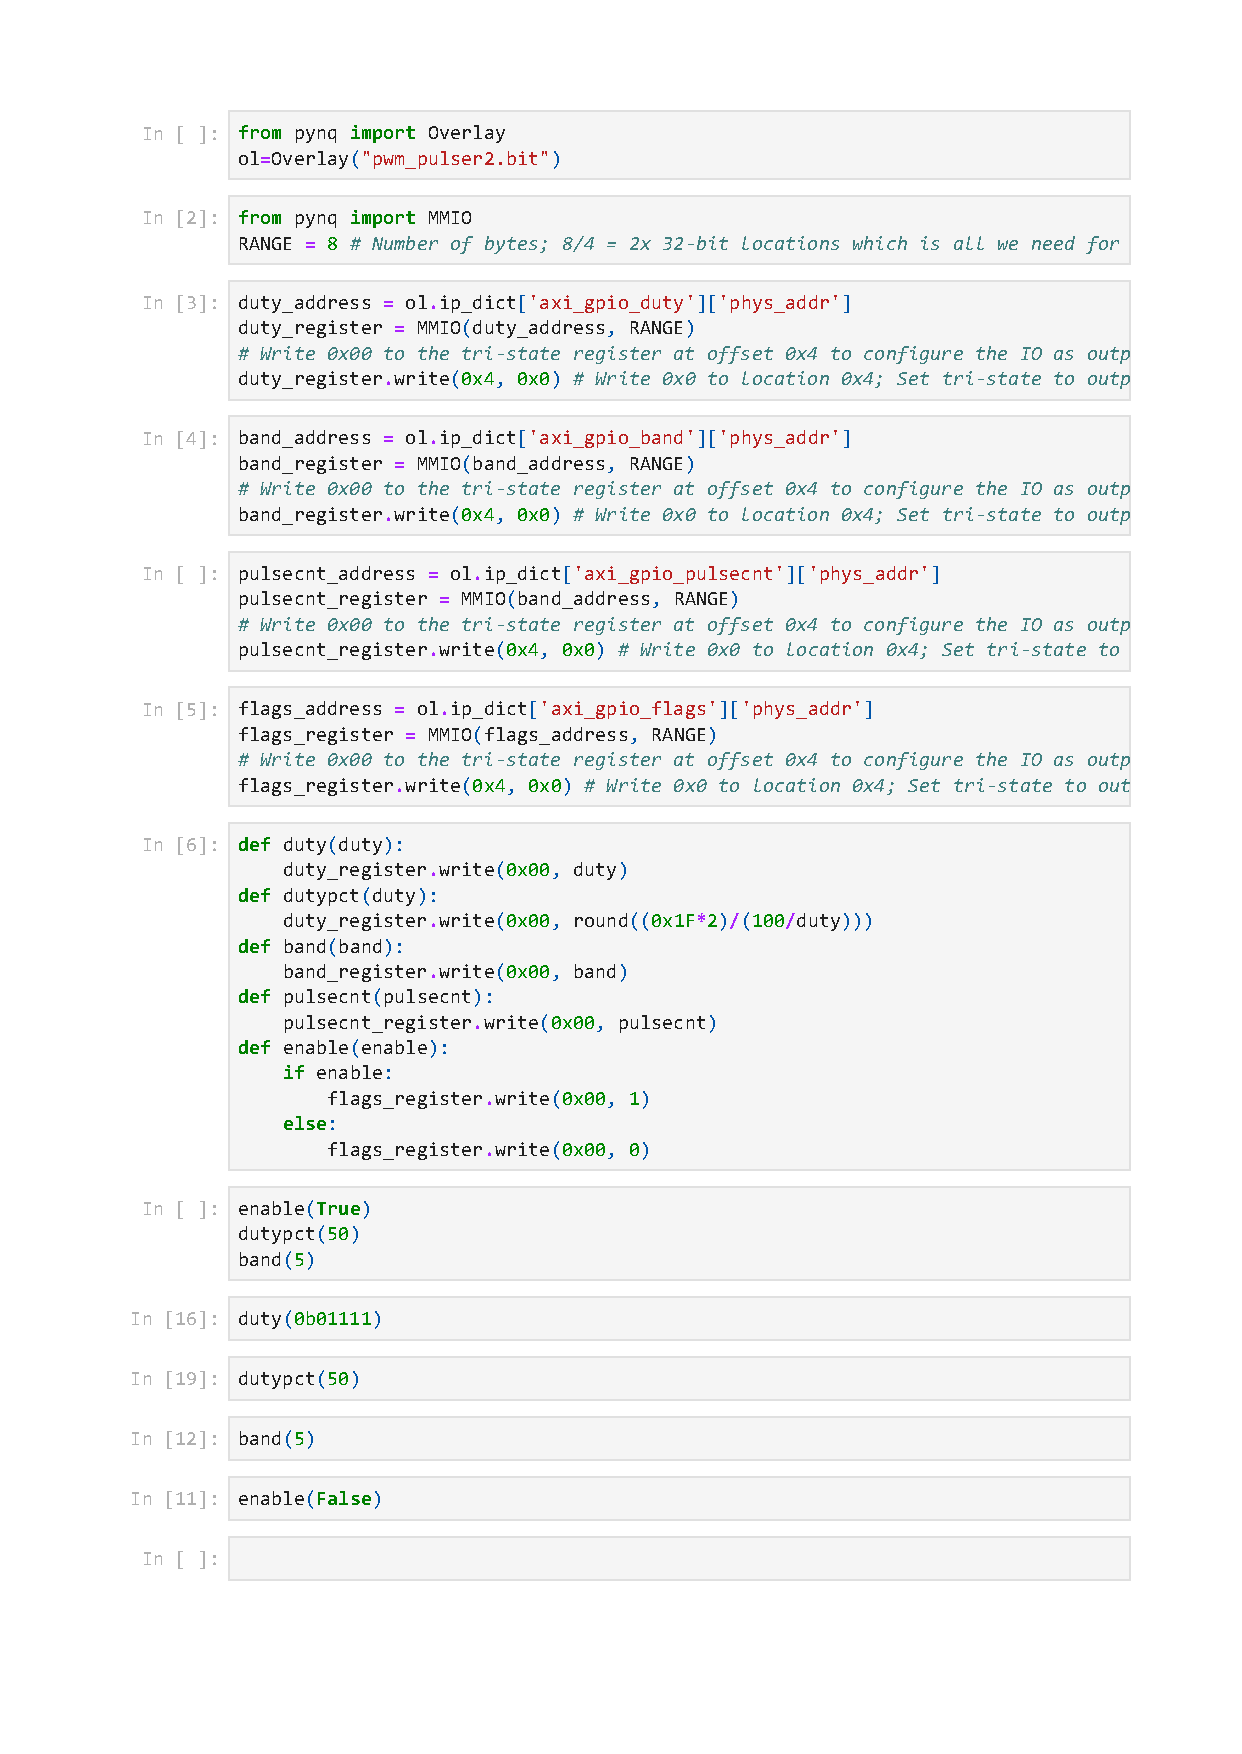
\includegraphics[height=.8\textheight]{Figures/appendix/fpga/pulser.pdf}
	\caption{Jupyter Notebook running on PYNQ Z1}
	\label{fig:app_jupyter_notebook}
\end{figure}
\begin{figure}[htbp!]
	\centering
	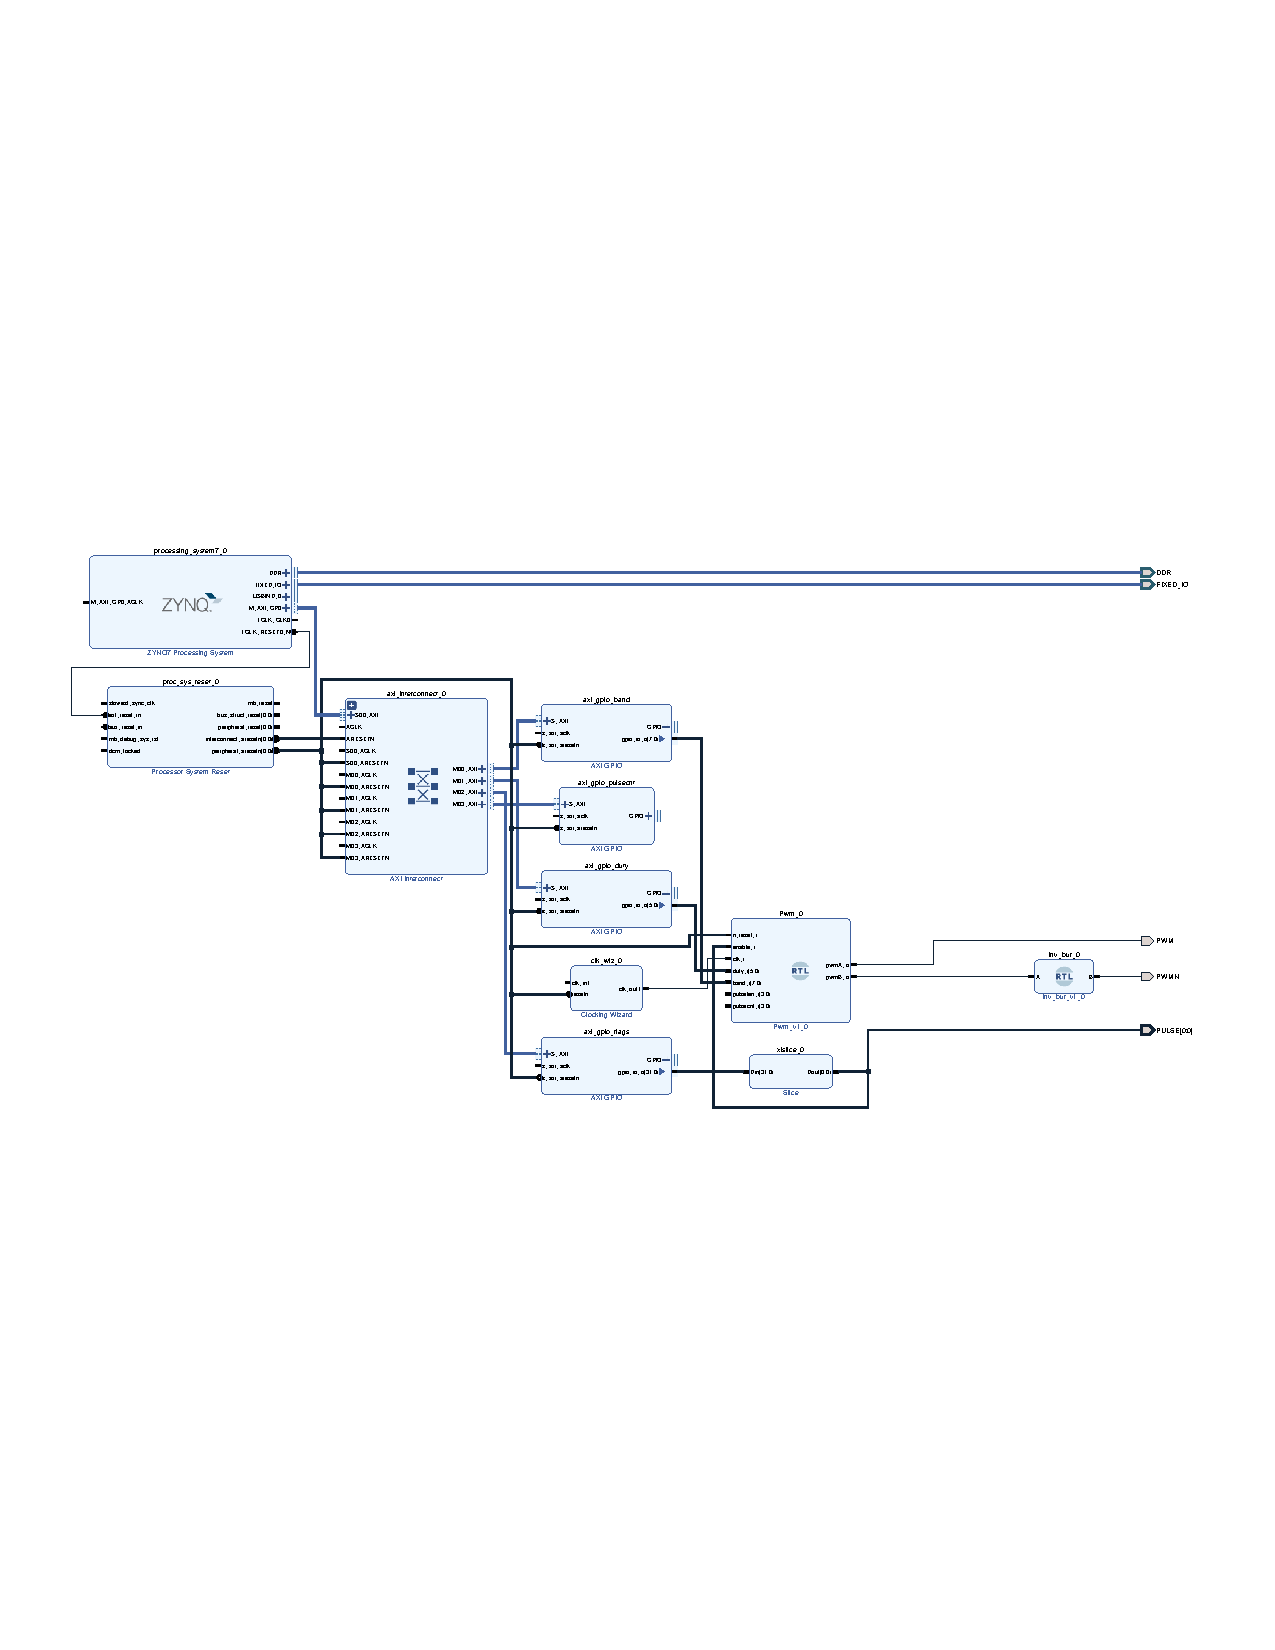
\includegraphics[width=\textwidth]{Figures/appendix/fpga/design_1.pdf}
	\caption{Block diagram of bitstream implementation}
	\label{fig:app_fpga_block_diagram}
\end{figure}
\begin{longlisting}
	\caption{Pwm.vhdl}
	\label{lst:Pwm.vhdl}
	\inputminted[bgcolor=LightGray,fontsize=\footnotesize,linenos,breaklines]{vhdl}{Figures/appendix/fpga/Pwm.vhdl}
\end{longlisting}
\begin{longlisting}
	\caption{signalcontroller.vhdl}
	\label{lst:signalcontroller.vhdl}
	\inputminted[bgcolor=LightGray,fontsize=\footnotesize,linenos,breaklines]{vhdl}{Figures/appendix/fpga/signalcontroller.vhdl}
\end{longlisting}
\begin{longlisting}
	\caption{inv\_top.vhdl}
	\label{lst:inv_top.vhdl}
	\inputminted[bgcolor=LightGray,fontsize=\footnotesize,linenos,breaklines]{vhdl}{Figures/appendix/fpga/inv_top.vhdl}
\end{longlisting}
\section{MATLAB Scripts}
\begin{longlisting}
	\caption{US Simulation Master Script.m}
	\label{lst:sim_master}
	\inputminted[bgcolor=LightGray,fontsize=\footnotesize,linenos,breaklines]{matlab}{Figures/appendix/matlab/US_Simulation_Master_Script.m}
\end{longlisting}

\begin{longlisting}
	\caption{Analysis.m}
	\label{lst:Analysis.m}
	\inputminted[bgcolor=LightGray,fontsize=\footnotesize,linenos,breaklines]{matlab}{Figures/appendix/matlab/Analysis.m}
\end{longlisting}

\begin{longlisting}
	\caption{demodulator.m}
	\label{lst:demodulator.m}
	\inputminted[bgcolor=LightGray,fontsize=\footnotesize,linenos,breaklines]{matlab}{Figures/appendix/matlab/demodulator.m}
\end{longlisting}

\begin{longlisting}
	\caption{preamplifier.m}
	\label{lst:preamplifier.m}
	\inputminted[bgcolor=LightGray,fontsize=\footnotesize,linenos,breaklines]{matlab}{Figures/appendix/matlab/preamplifier.m}
\end{longlisting}

\begin{longlisting}
	\caption{sampler.m}
	\label{lst:sampler.m}
	\inputminted[bgcolor=LightGray,fontsize=\footnotesize,linenos,breaklines]{matlab}{Figures/appendix/matlab/sampler.m}
\end{longlisting}

\begin{longlisting}
	\caption{transmitter.m}
	\label{lst:transmitter.m}
	\inputminted[bgcolor=LightGray,fontsize=\footnotesize,linenos,breaklines]{matlab}{Figures/appendix/matlab/transmitter.m}
\end{longlisting}

\begin{longlisting}
	\caption{vna.m}
	\label{lst:vna.m}
	\inputminted[bgcolor=LightGray,fontsize=\footnotesize,linenos,breaklines]{matlab}{Figures/appendix/matlab/vna.m}
\end{longlisting}

\begin{longlisting}
	\caption{bpf datasheet s21.m}
	\label{lst:bpf_datasheet_s21.m}
	\inputminted[bgcolor=LightGray,fontsize=\footnotesize,linenos,breaklines]{matlab}{Figures/appendix/matlab/datasheet_s21.m}
\end{longlisting}

\begin{longlisting}
	\caption{switch.m}
	\label{lst:switch.m}
	\inputminted[bgcolor=LightGray,fontsize=\footnotesize,linenos,breaklines]{matlab}{Figures/appendix/matlab/Switch_demo.m}
\end{longlisting}


\chapter{Simulation Models}
\begin{figure}[htbp]
	\centering
	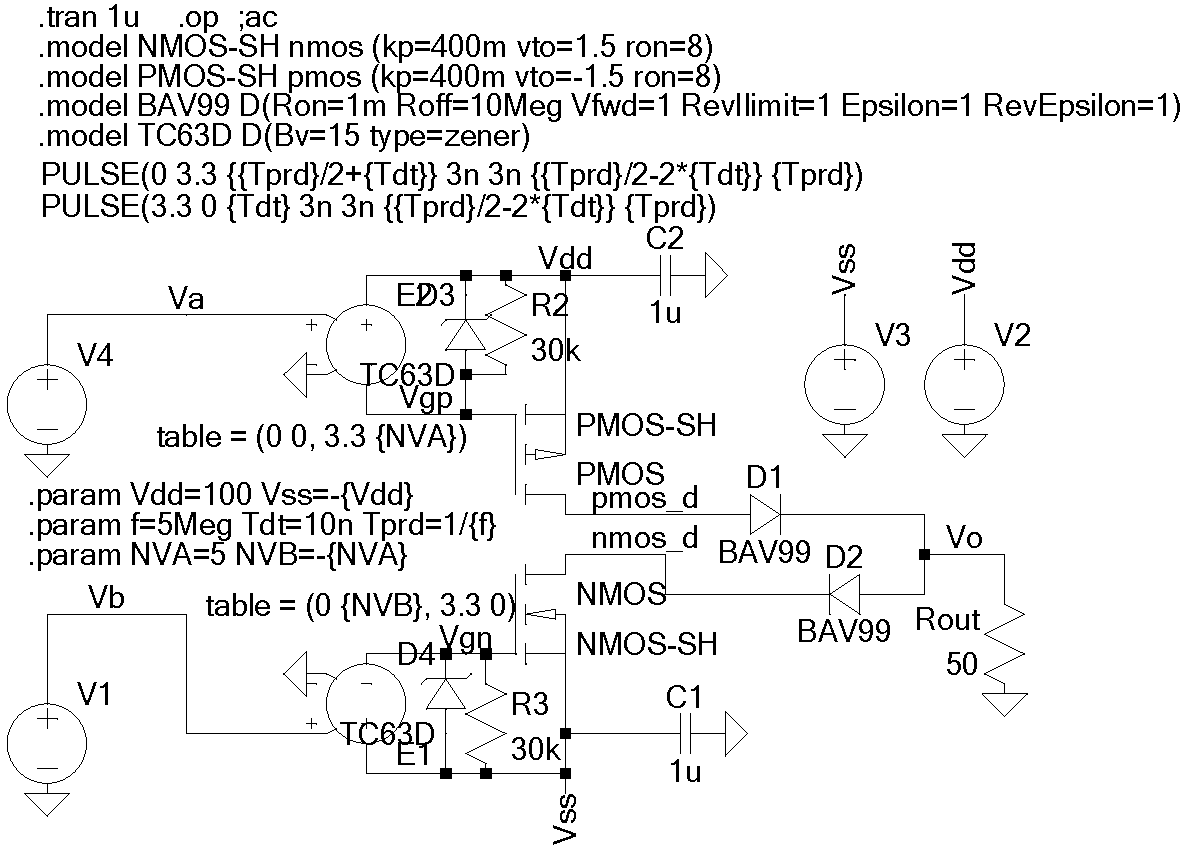
\includegraphics[width=.9\textwidth]{Figures/appendix/ltspice_transmitter.pdf}
	\caption{LTspice model of transmitter}
	\label{fig:app_ltspice_transmitter}
\end{figure}
\begin{figure}[htbp]
	\centering
	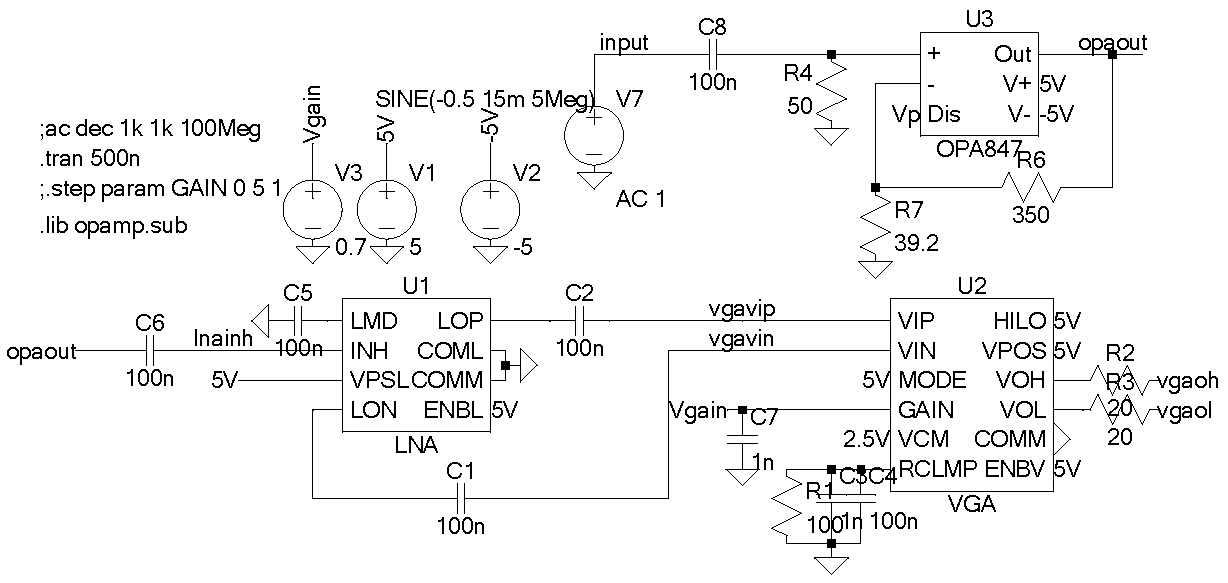
\includegraphics[width=.9\textwidth]{Figures/appendix/ltspice_preamp.pdf}
	\caption{LTspice model of preamplifier}
	\label{fig:app_ltspice_preamp}
\end{figure}
\begin{figure}[htbp]
	\centering
	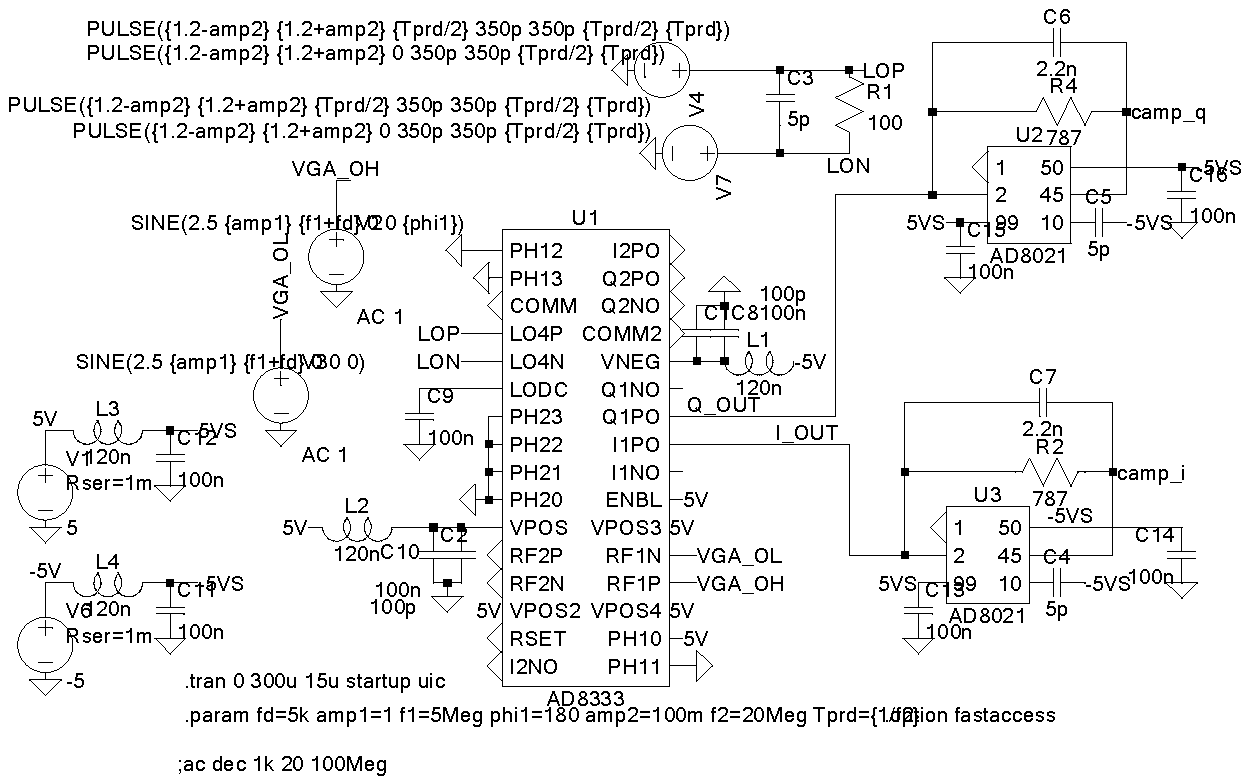
\includegraphics[width=.9\textwidth]{Figures/appendix/ltspice_demod.pdf}
	\caption{LTspice model of demodulator}
	\label{fig:app_ltspice_demod}
\end{figure}
\begin{figure}[htbp]
	\centering
	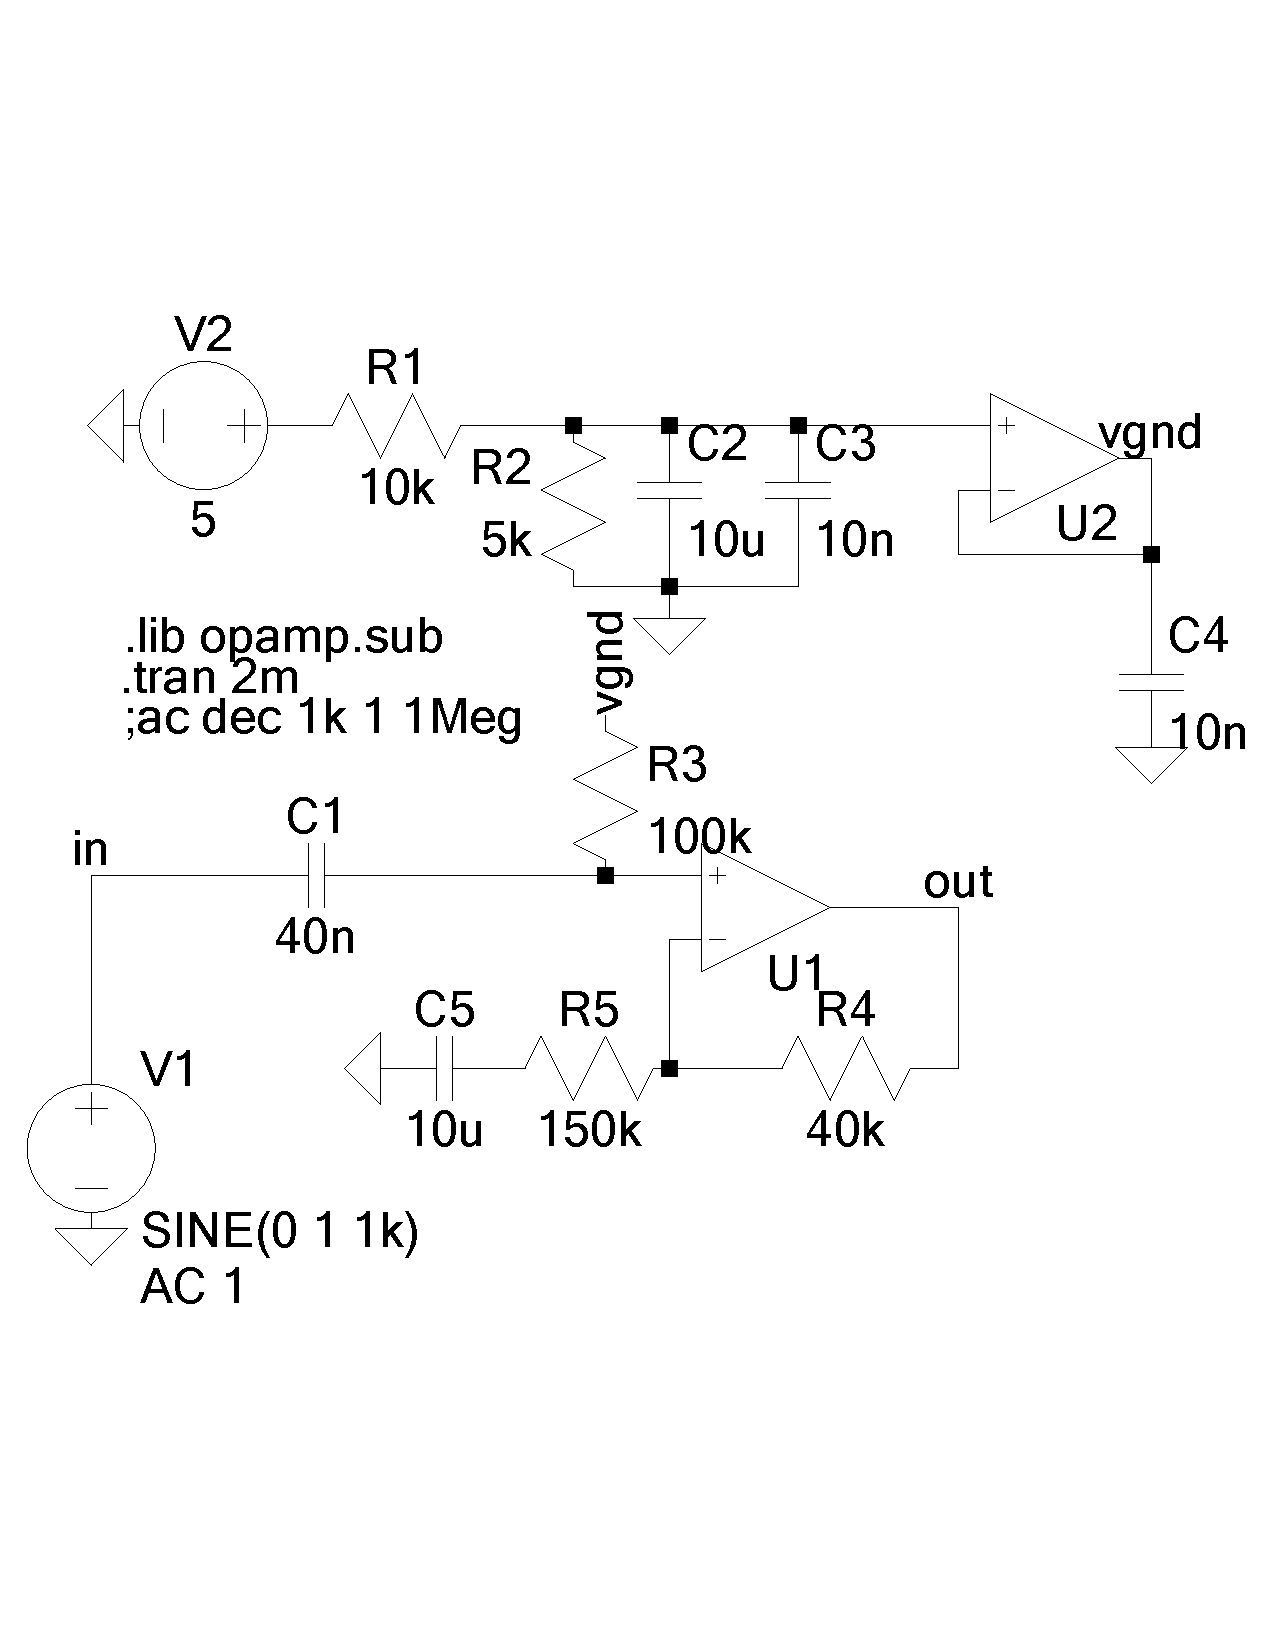
\includegraphics[width=.9\textwidth]{Figures/appendix/ltspice_dccoupler.pdf}
	\caption{LTspice model of PRF filter}
	\label{fig:app_ltspice_dc_coupler}
\end{figure}


%\chapter{Timer Configurations}
%\begin{figure}[htbp]
%	\centering
%	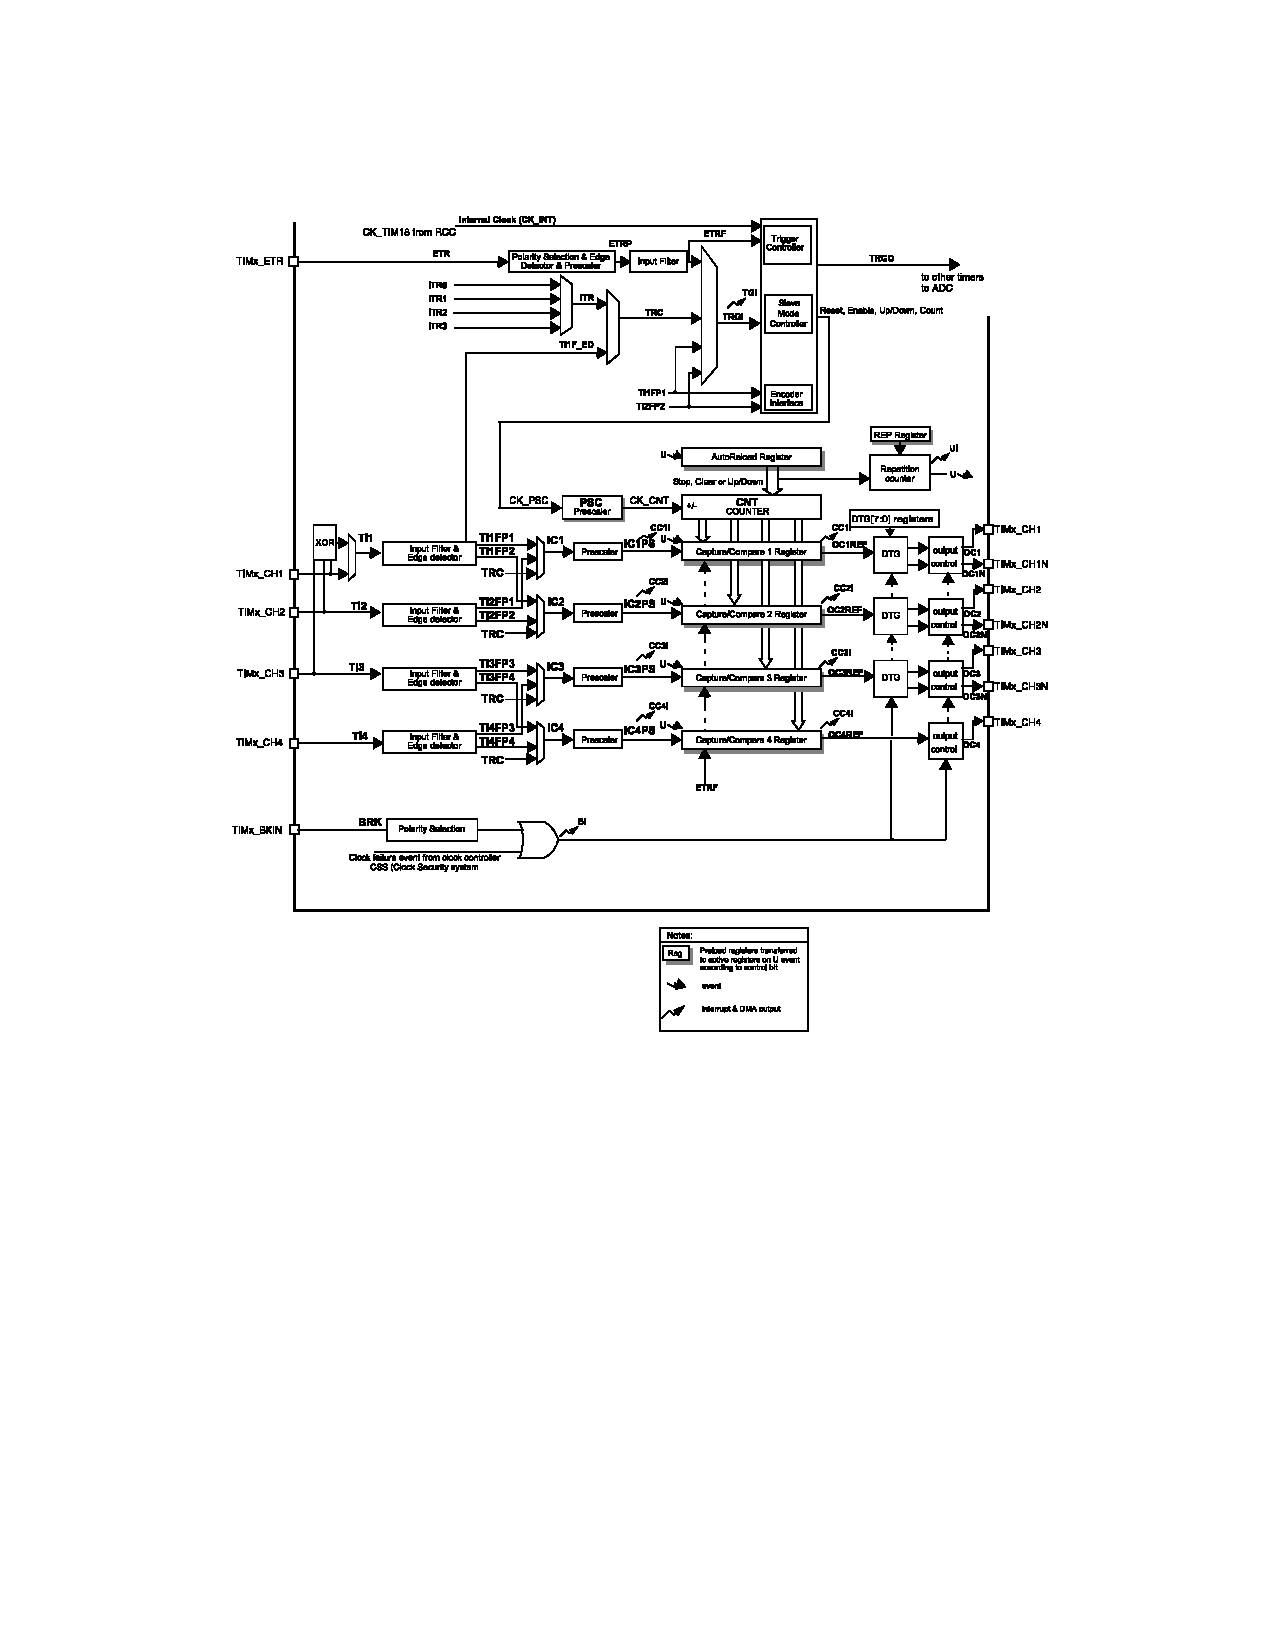
\includegraphics[width=.8\textwidth]{Figures/4_advanced_timer1_diagram.pdf}
%	\caption{Configuration of \texttt{TIMER1}}
%	\label{fig:4_timer1}
%\end{figure}
%\begin{figure}[htbp]
%	\centering
%	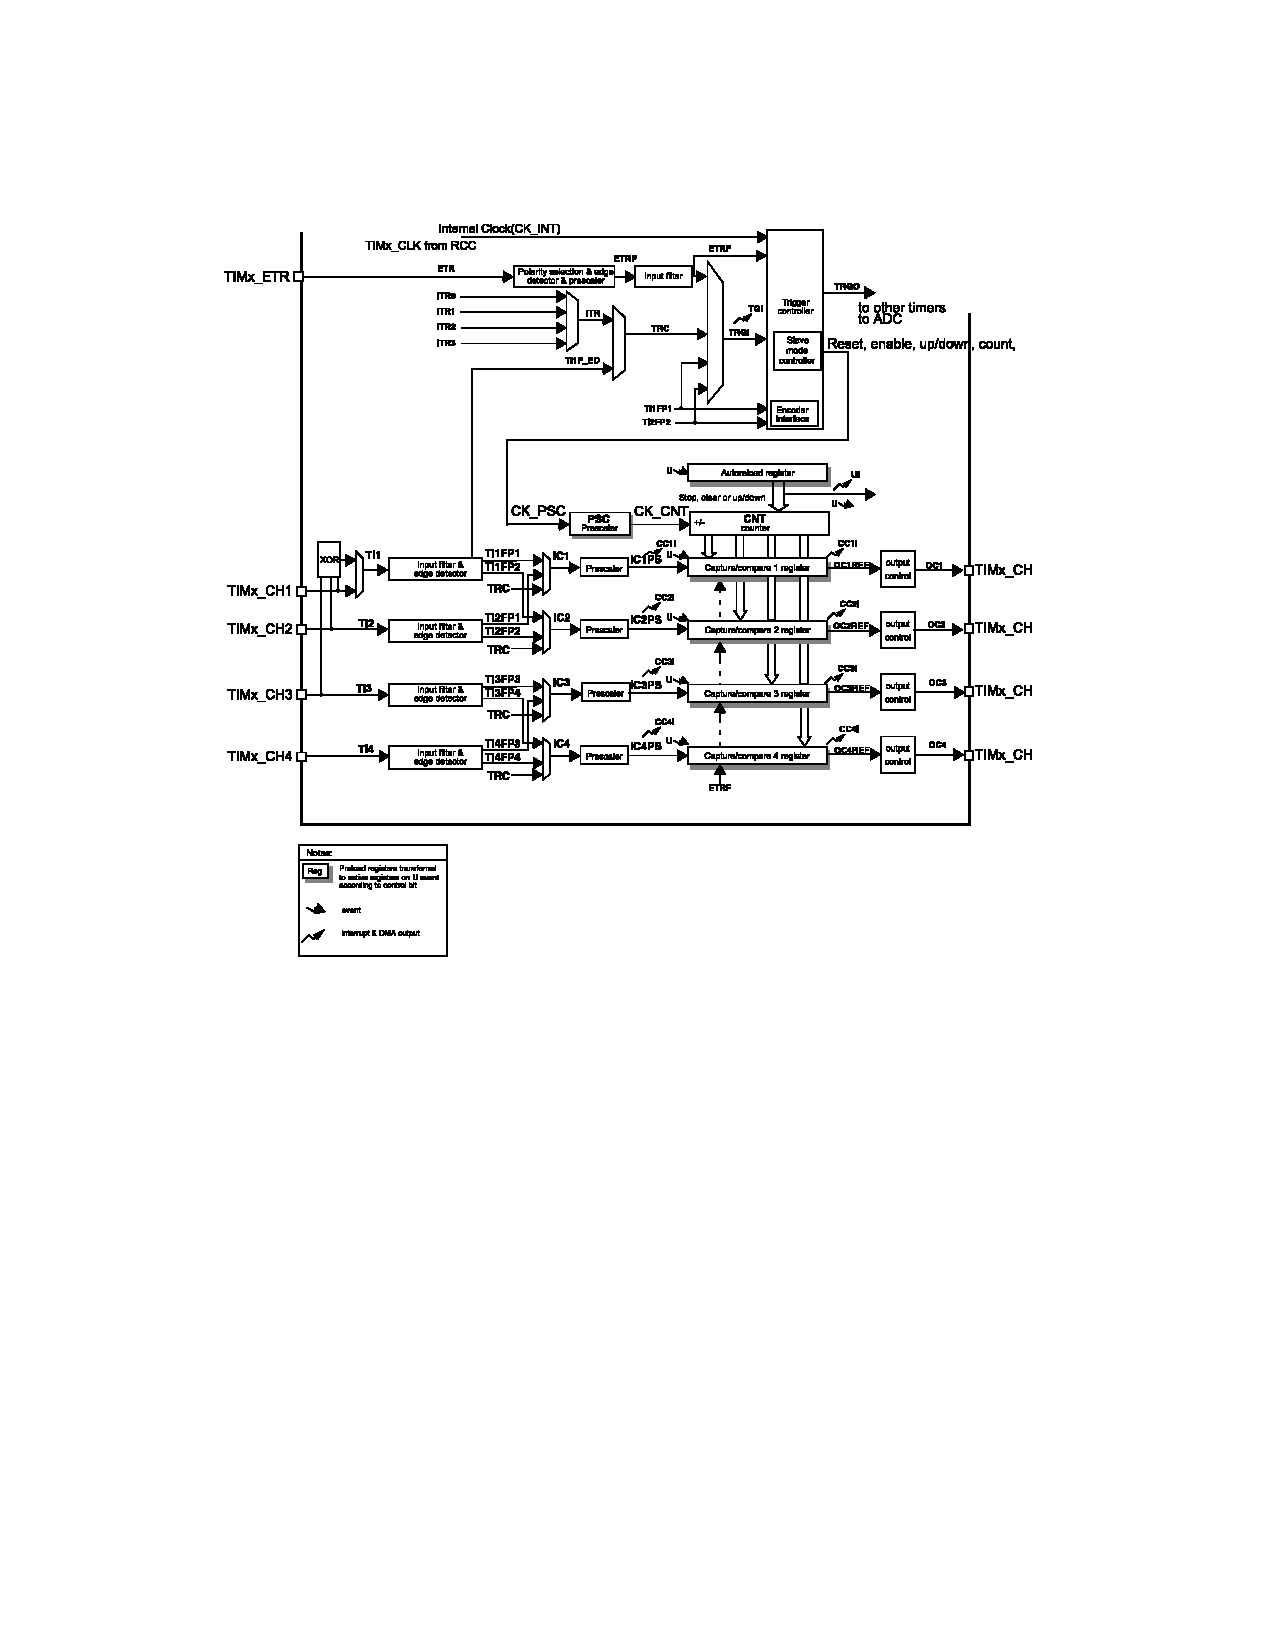
\includegraphics[width=.8\textwidth]{Figures/4_advanced_timer2-5_diagram.pdf}
%	\caption{Configuration of \texttt{TIMER2--5}}
%	\label{fig:4_timer2-5}
%\end{figure}
%\begin{figure}[htbp]
%	\centering
%	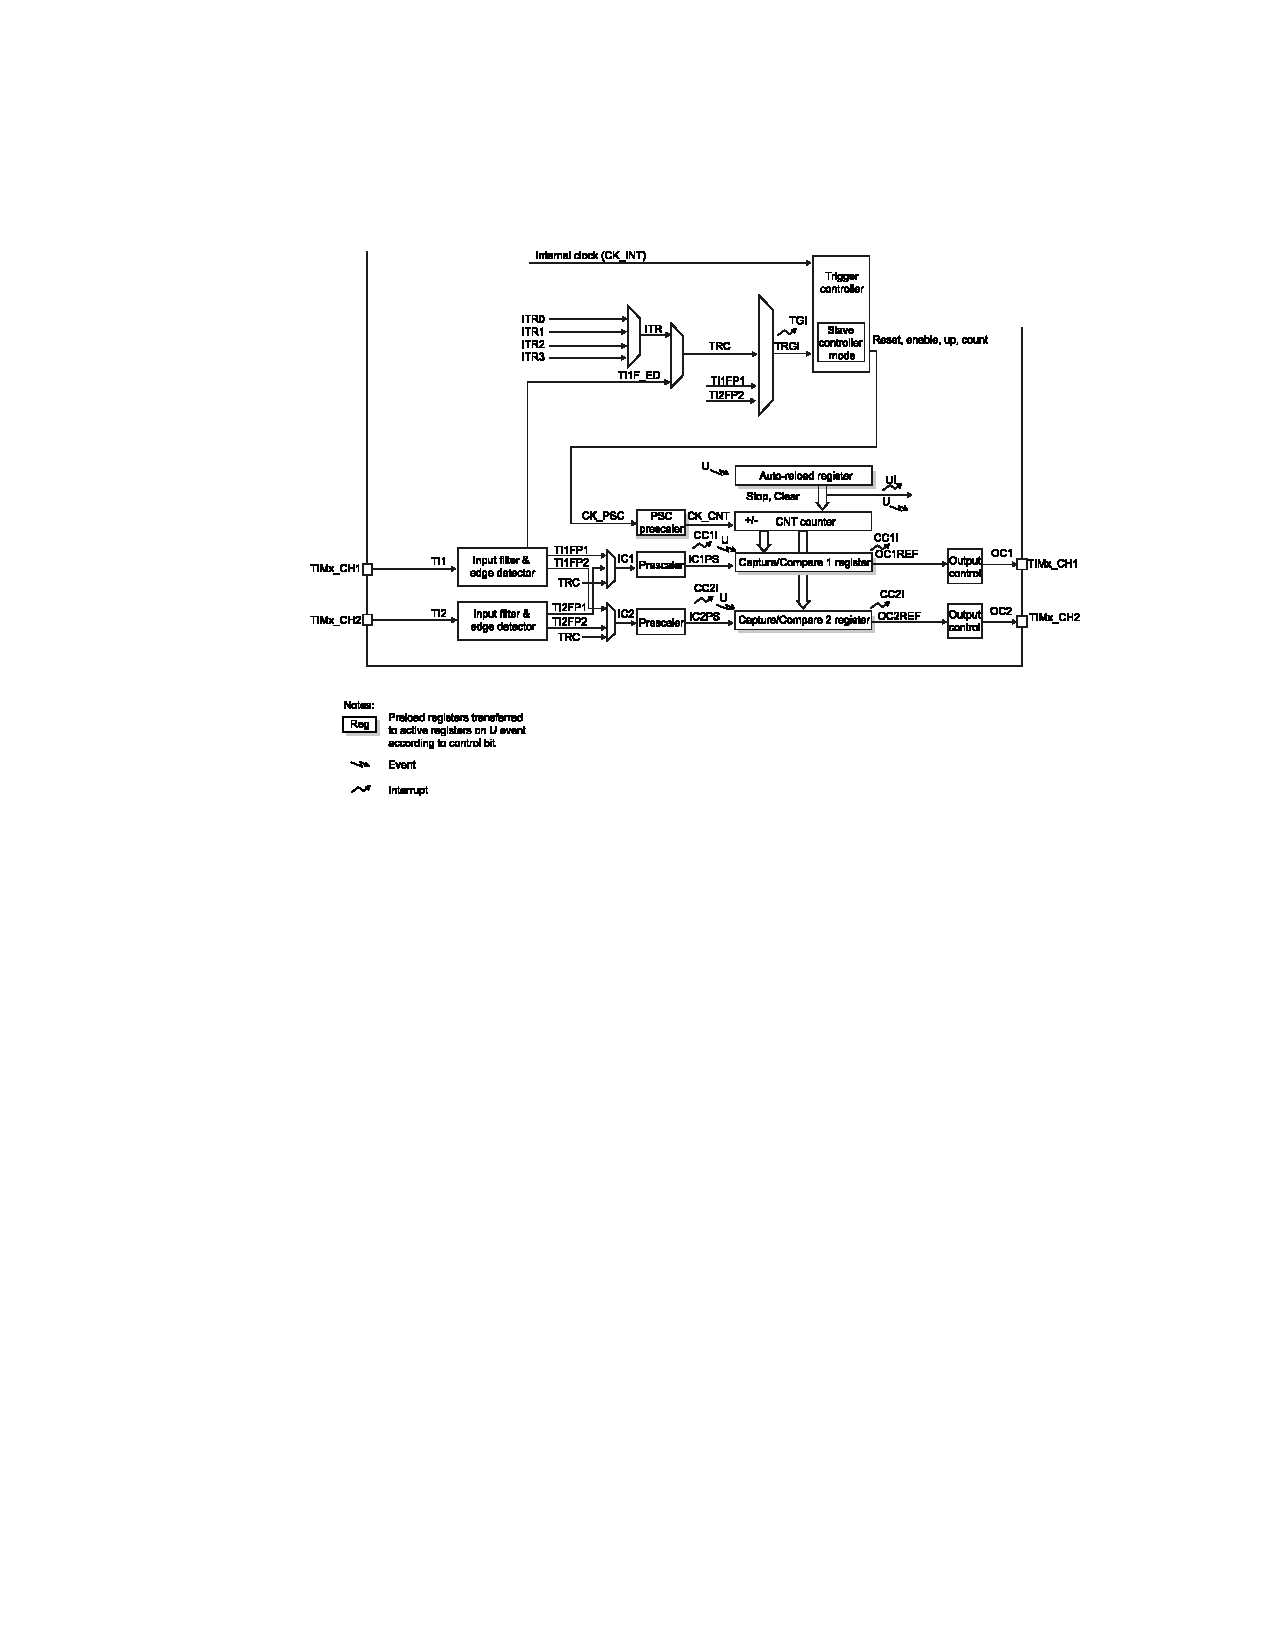
\includegraphics[width=.8\textwidth]{Figures/4_advanced_timer9_diagram.pdf}
%	\caption{Configuration of \texttt{TIMER9}}
%	\label{fig:4_timer9}
%\end{figure}


\chapter{Circuit Schematics}
\begin{landscape}
	\begin{figure}[htbp]
		\centering
		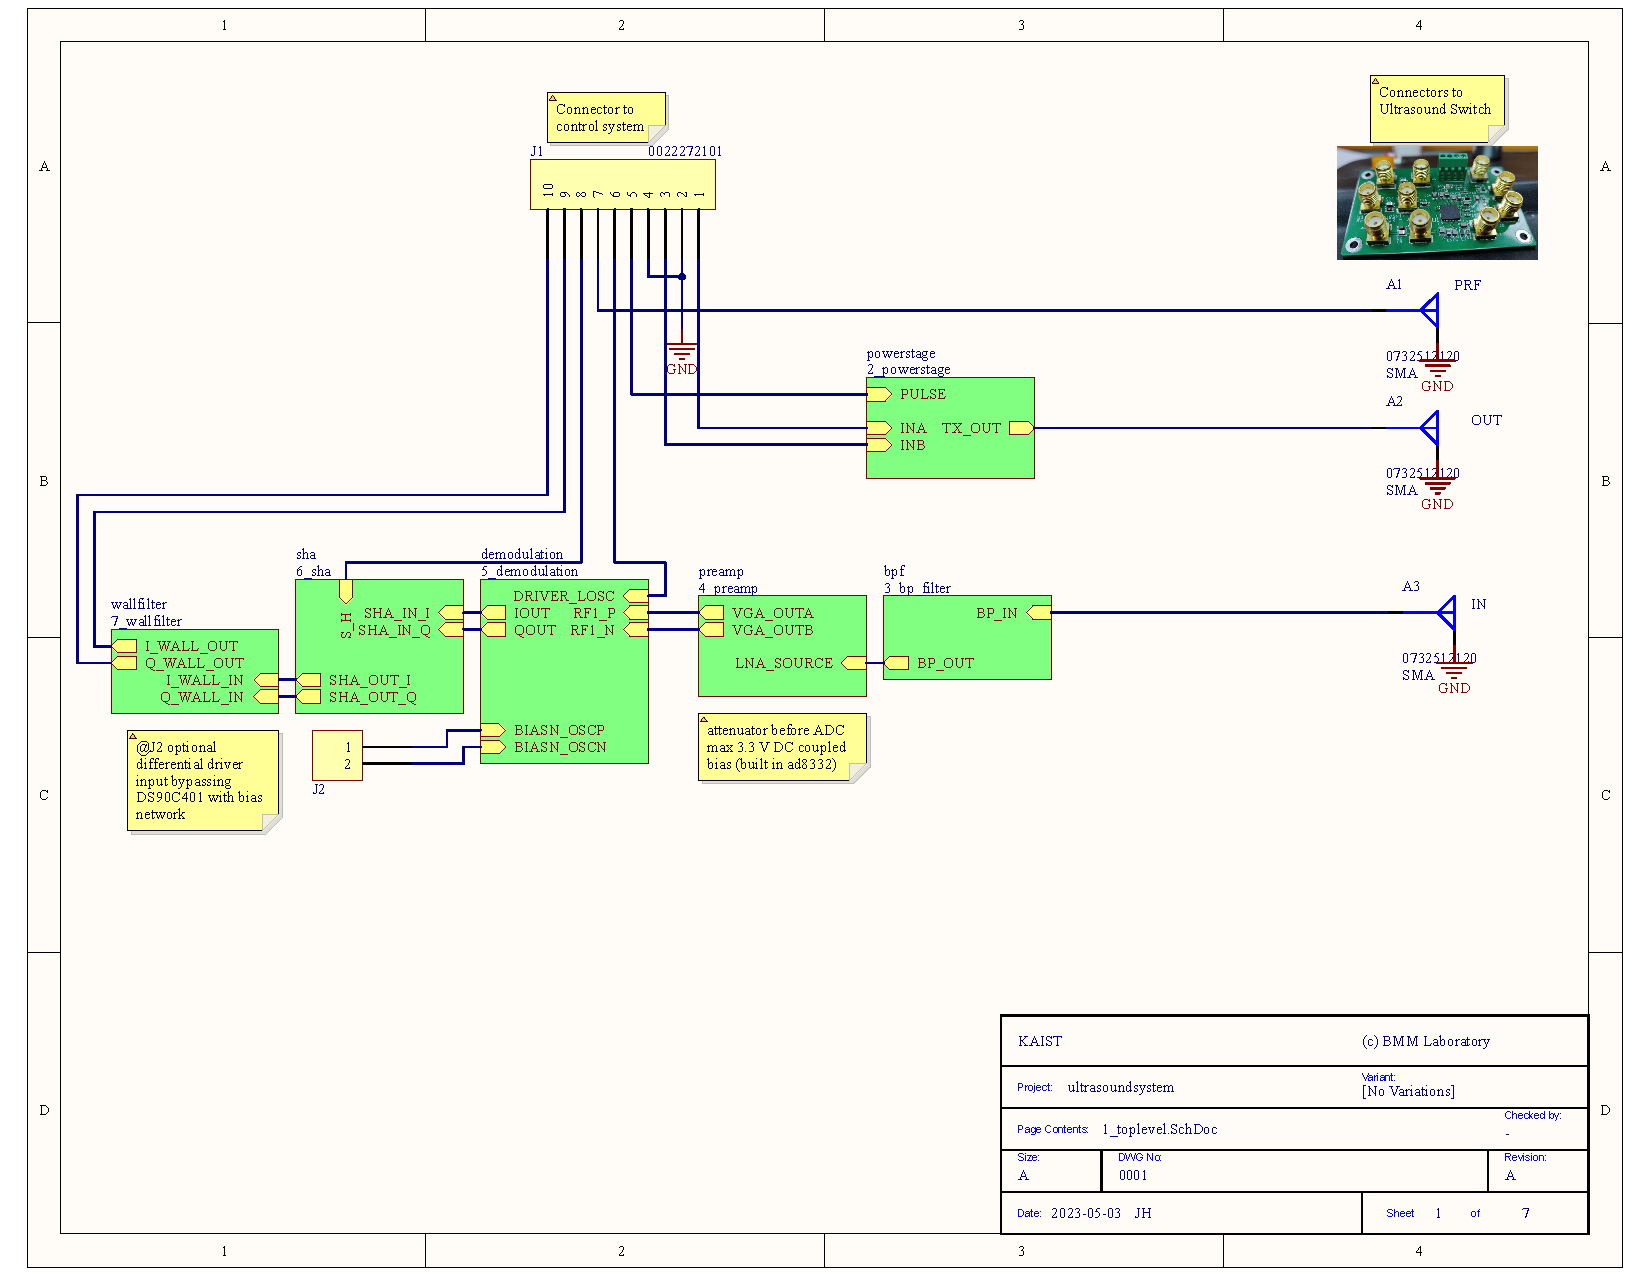
\includegraphics[width=20cm,height=28.7cm,keepaspectratio]{Figures/appendix/afe_altium/1_toplevel.pdf}
		\caption{AFE Top Level}
		\label{fig:appendix_1_toplevel}
	\end{figure}
\end{landscape}
\begin{landscape}
	\begin{figure}[htbp]
		\centering
		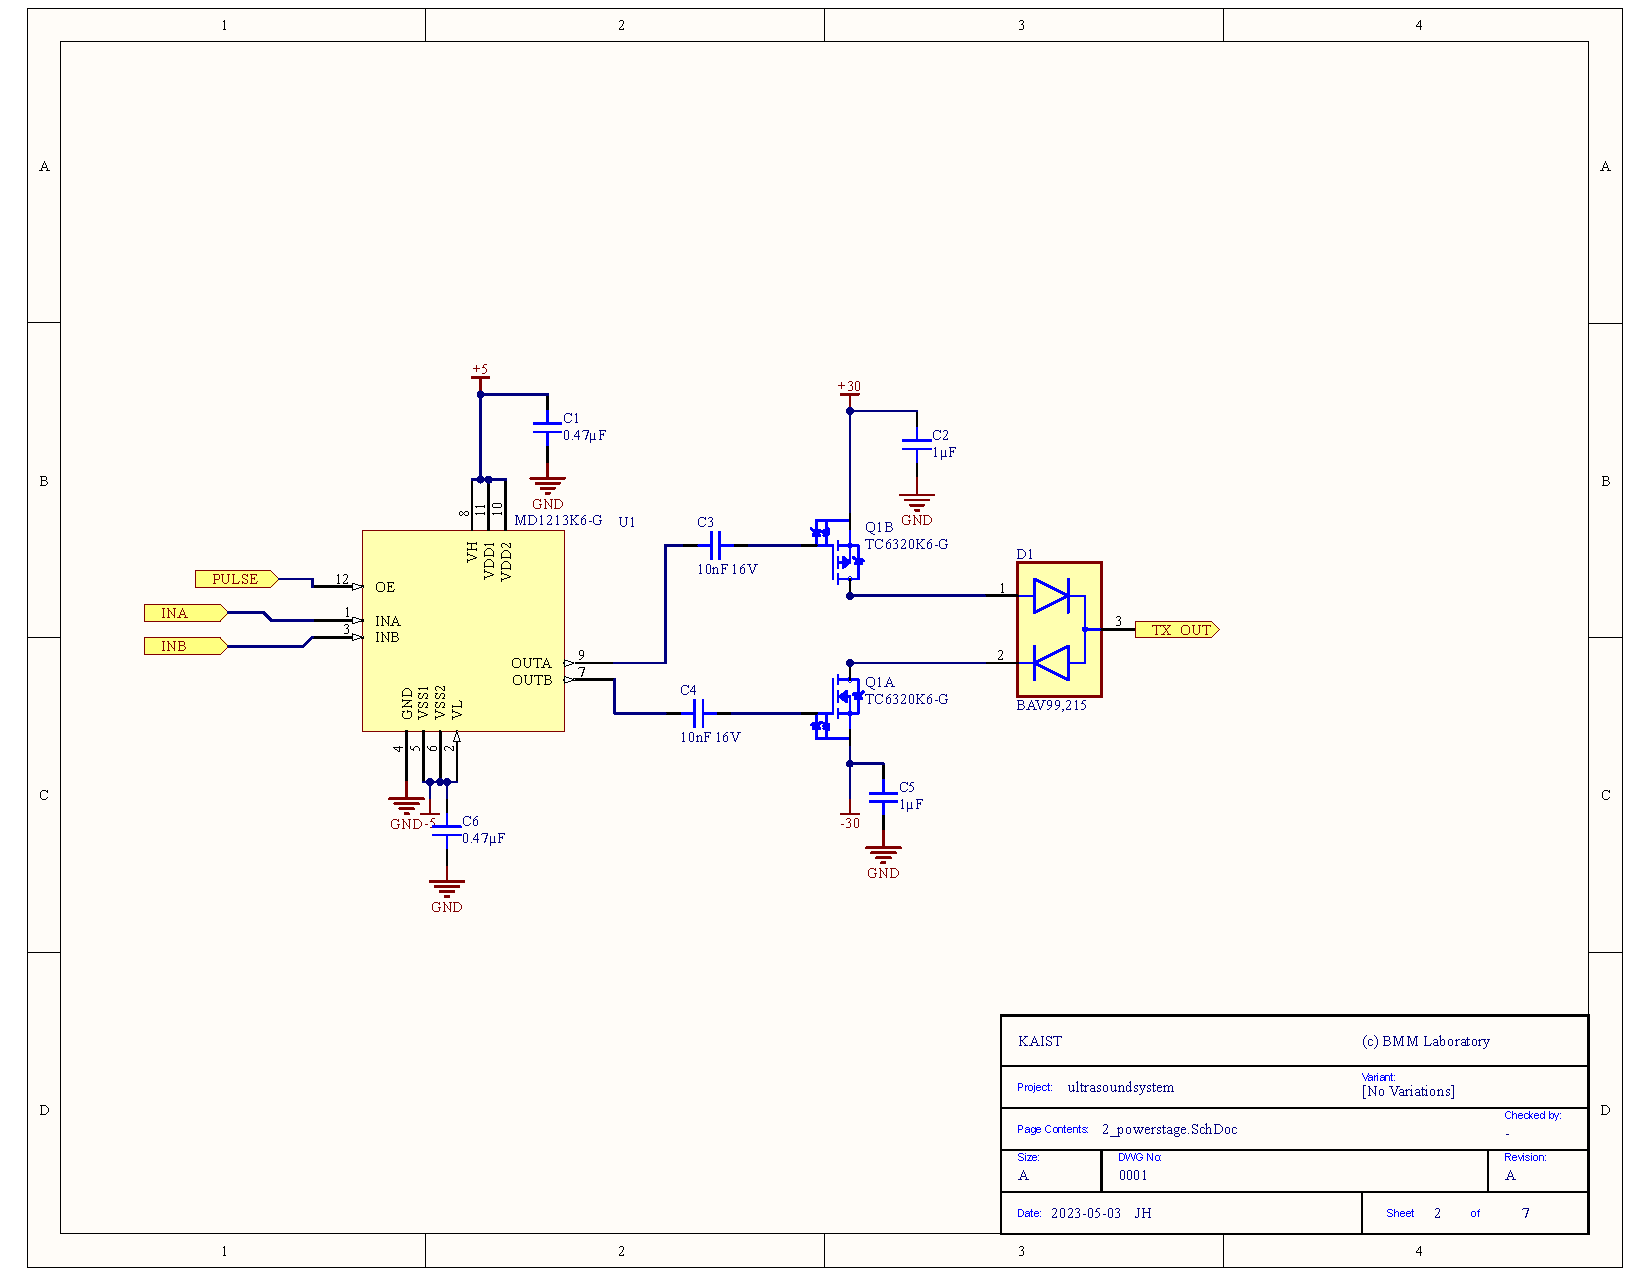
\includegraphics[width=20cm,height=28.7cm,keepaspectratio]{Figures/appendix/afe_altium/2_powerstage.pdf}
		\caption{AFE Power Stage}
		\label{fig:appendix_2_powerstage}
	\end{figure}
\end{landscape}
\begin{landscape}
	\begin{figure}[htbp]
		\centering
		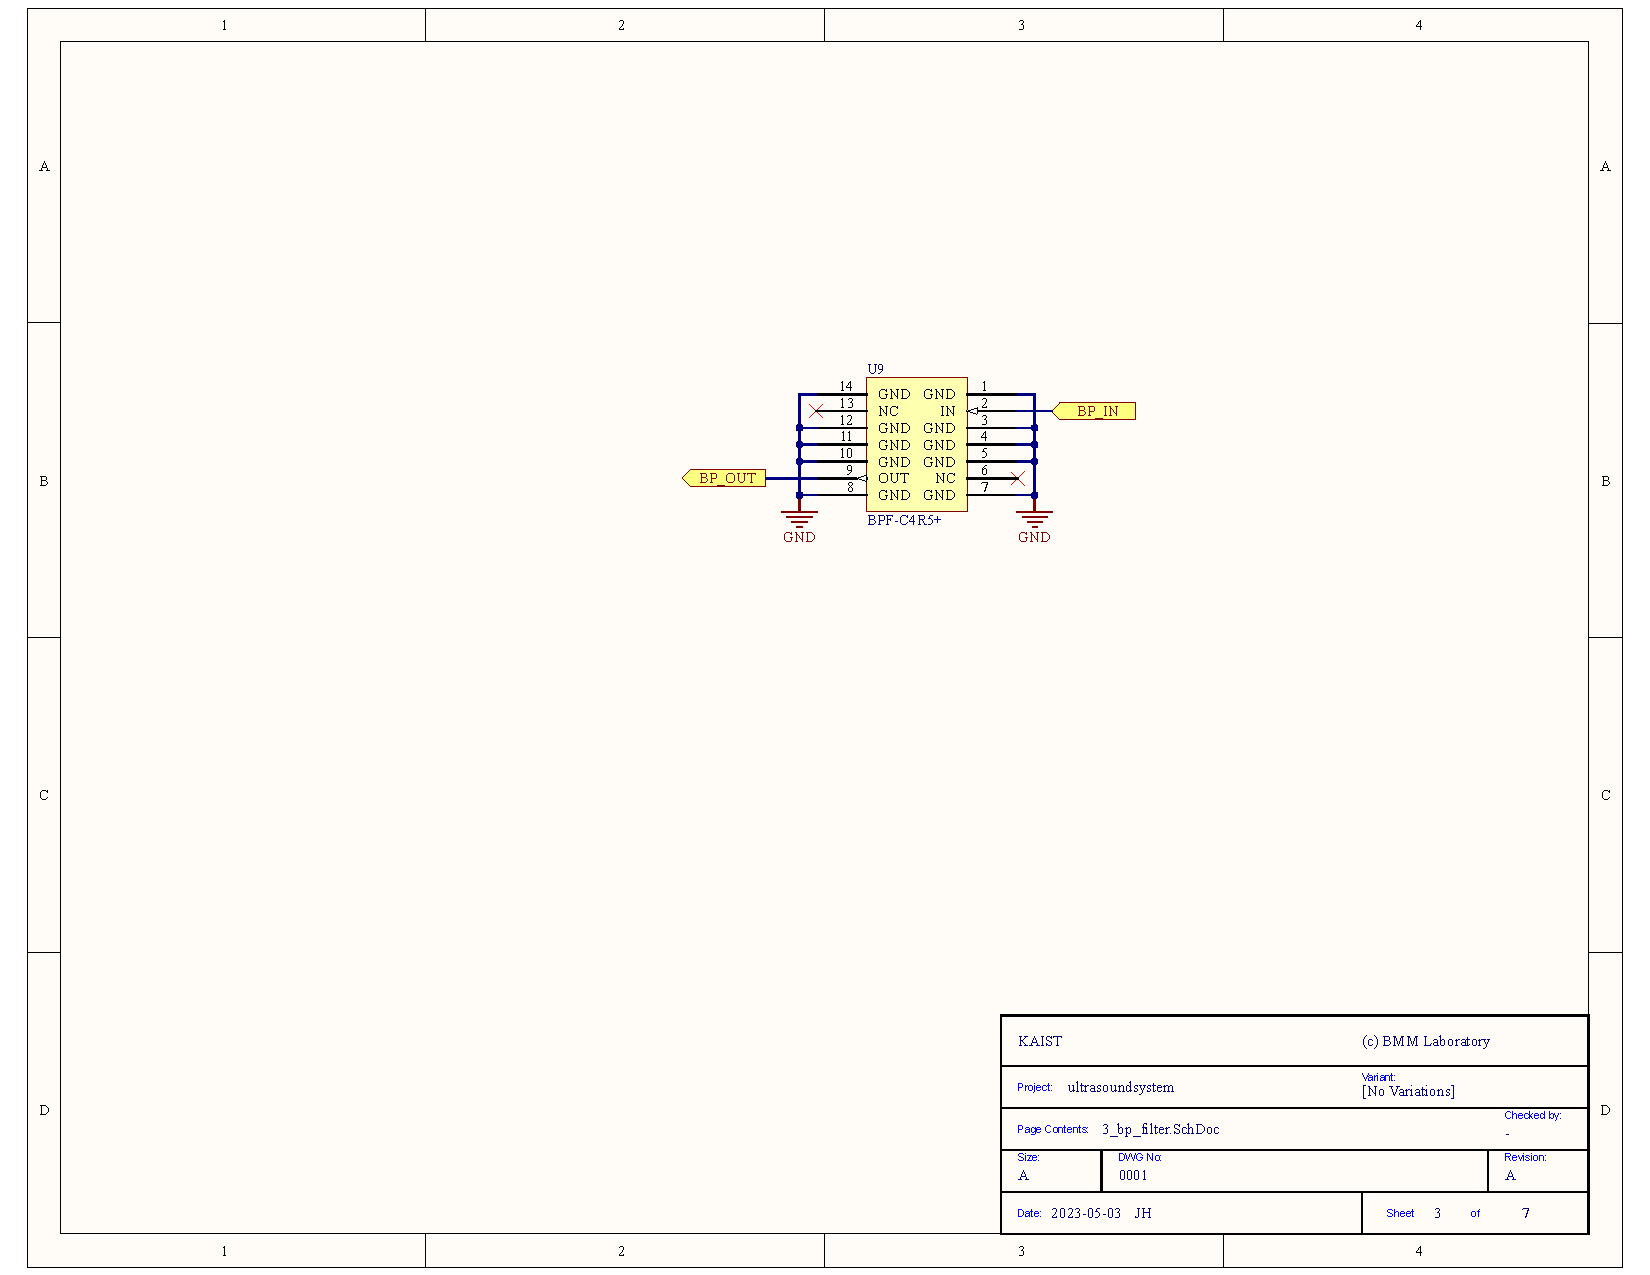
\includegraphics[width=20cm,height=28.7cm,keepaspectratio]{Figures/appendix/afe_altium/3_bpf.pdf}
		\caption{AFE BPF}
		\label{fig:appendix_3_bpf}
	\end{figure}
\end{landscape}
\begin{landscape}
	\begin{figure}[htbp]
		\centering
		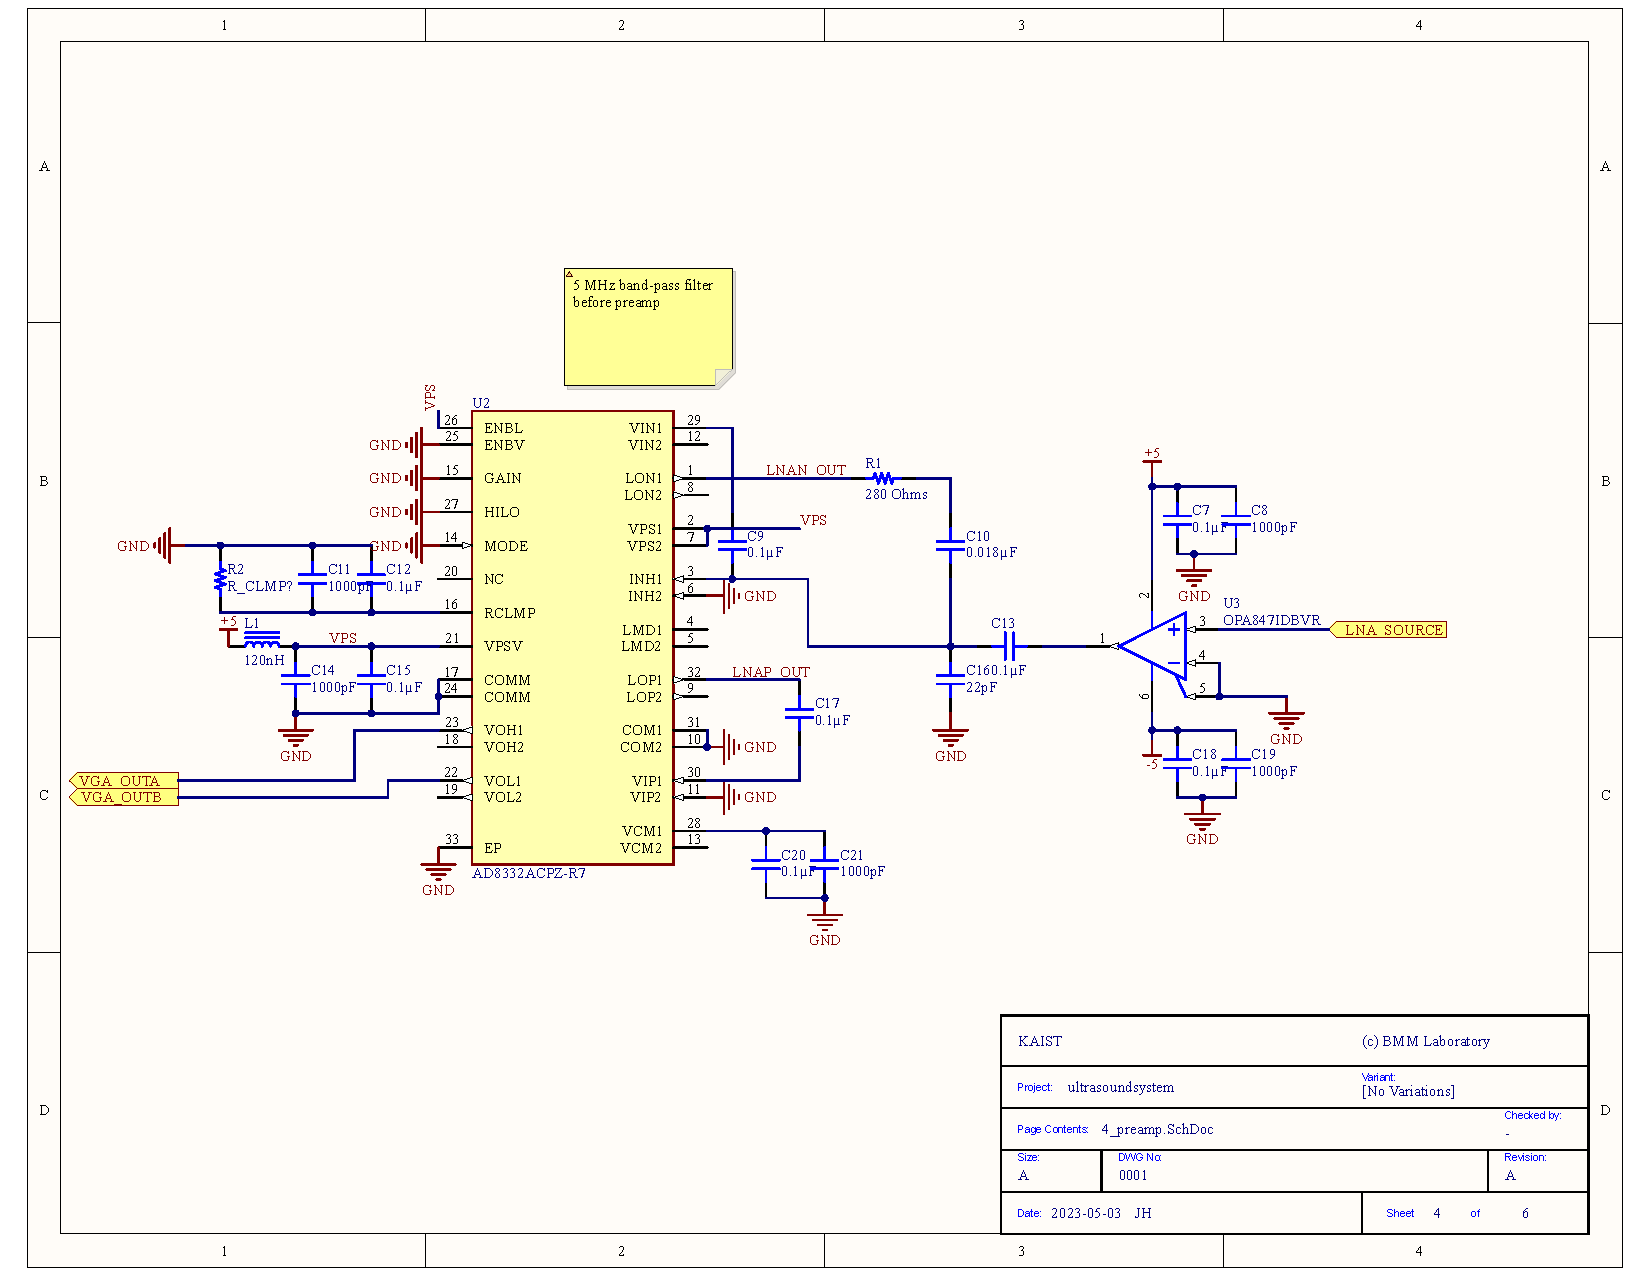
\includegraphics[width=20cm,height=28.7cm,keepaspectratio]{Figures/appendix/afe_altium/4_preamp.pdf}
		\caption{AFE Preamplifier}
		\label{fig:appendix_4_preamp}
	\end{figure}
\end{landscape}
\begin{landscape}
	\begin{figure}[htbp]
		\centering
		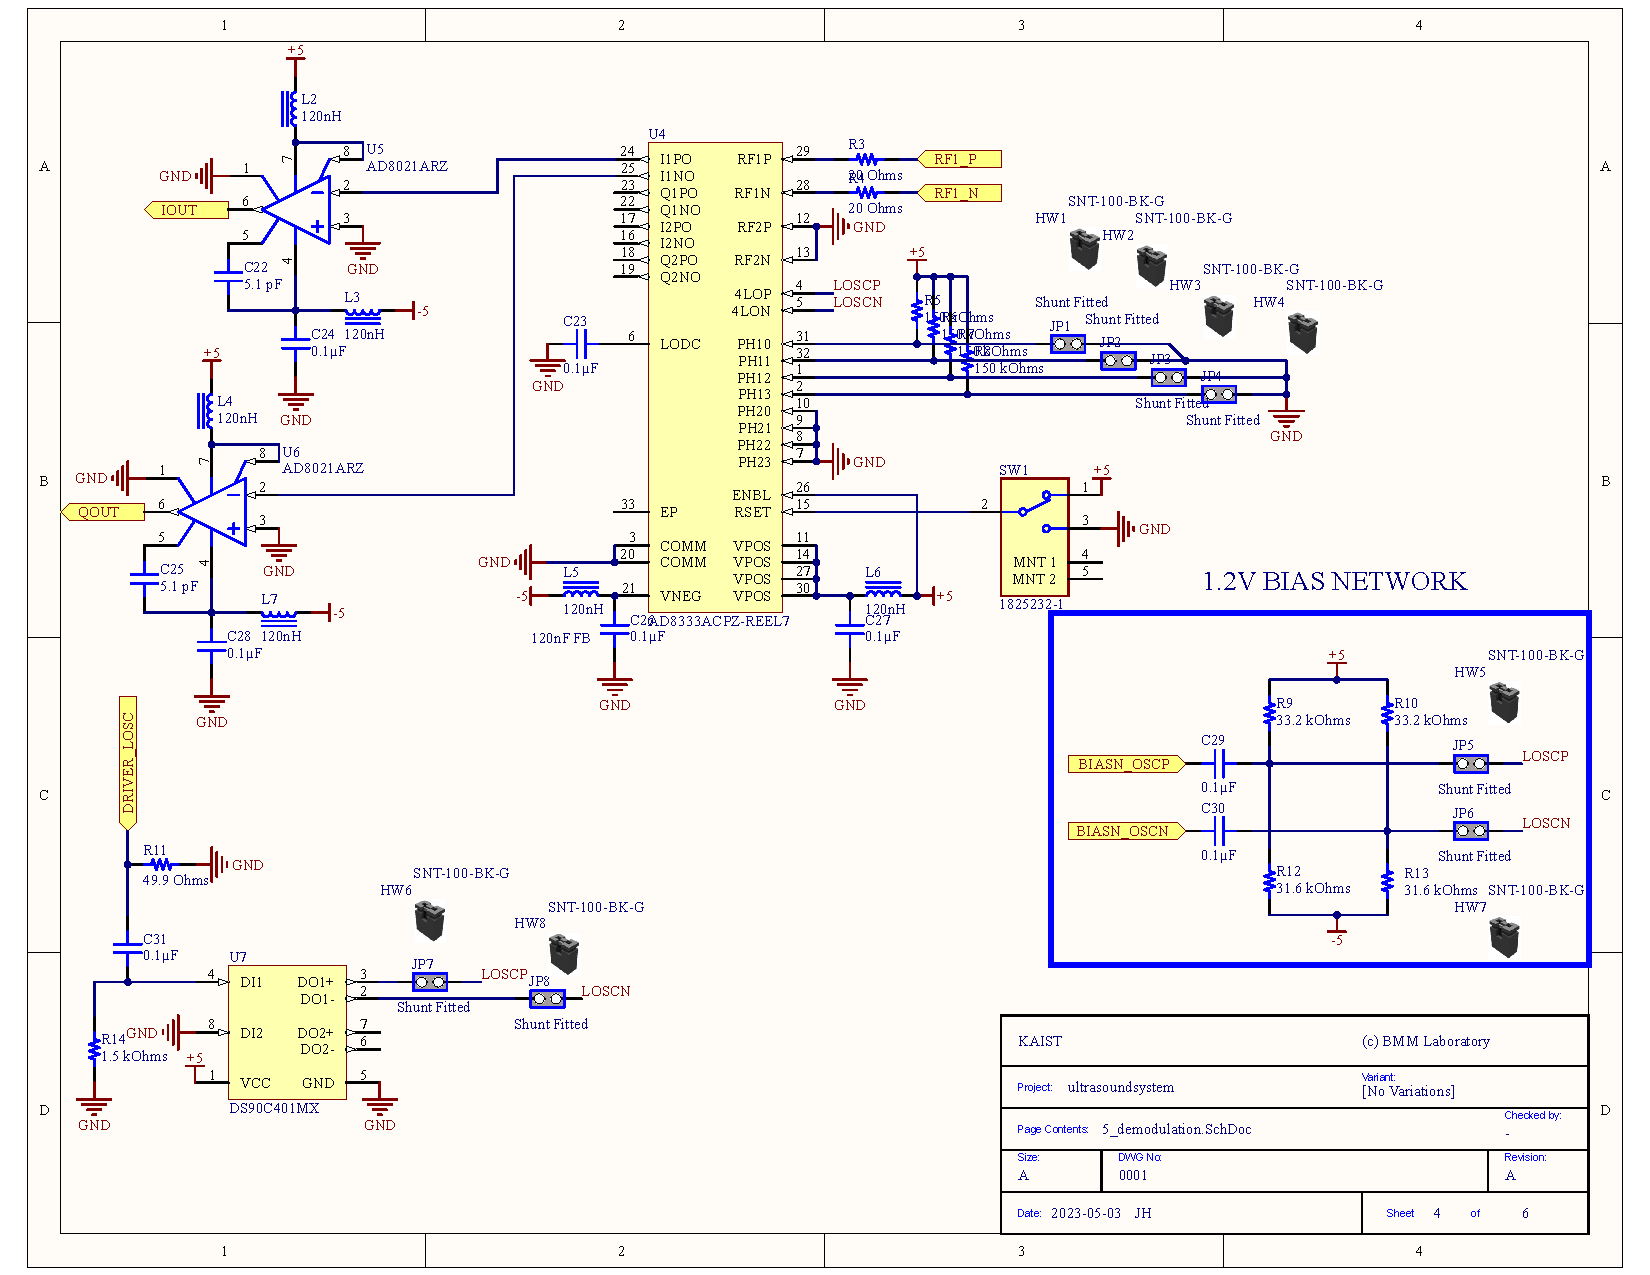
\includegraphics[width=20cm,height=28.7cm,keepaspectratio]{Figures/appendix/afe_altium/5_demodulator.pdf}
		\caption{AFE Demodulator}
		\label{fig:appendix_5_demodulator}
	\end{figure}
\end{landscape}
\begin{landscape}
	\begin{figure}[htbp]
		\centering
		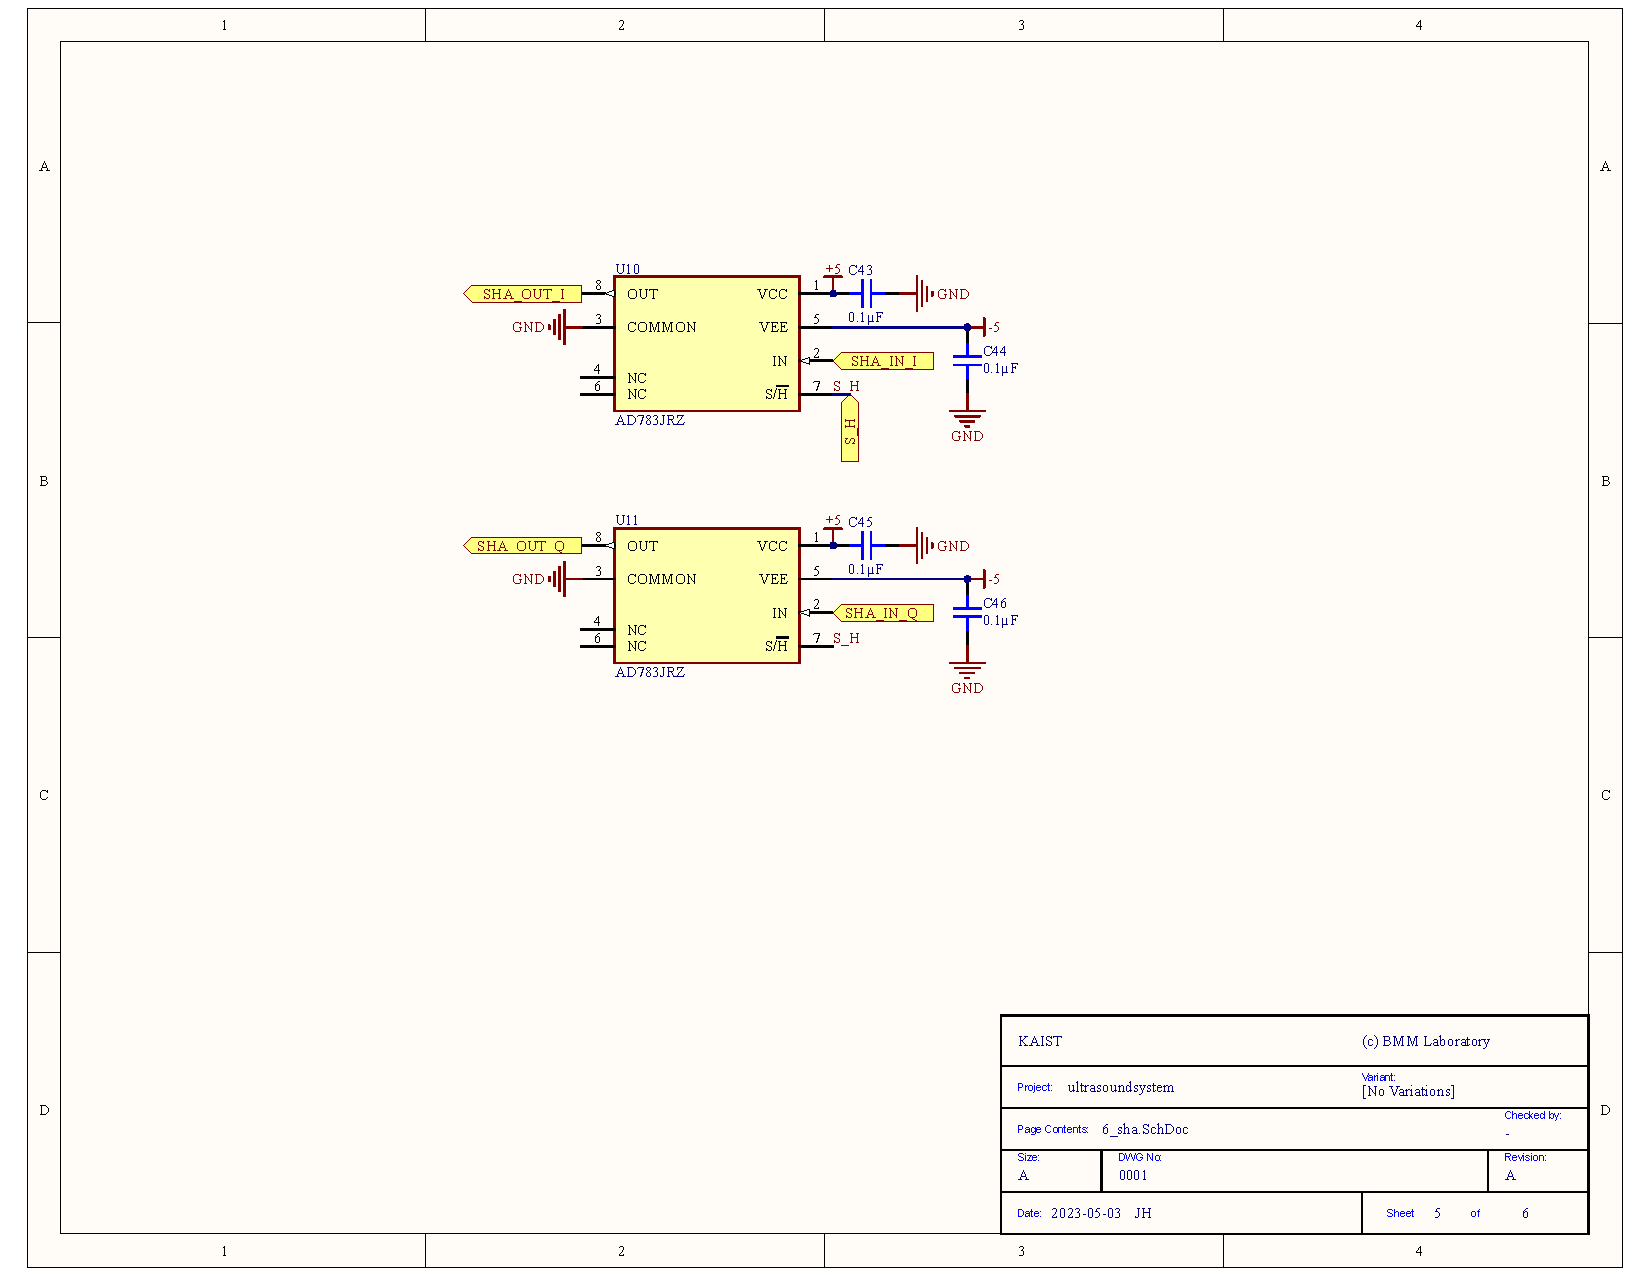
\includegraphics[width=20cm,height=28.7cm,keepaspectratio]{Figures/appendix/afe_altium/6_sha.pdf}
		\caption{AFE Sample and Hold Amplifier}
		\label{fig:appendix_6_sha}
	\end{figure}
\end{landscape}
\begin{landscape}
	\begin{figure}[htbp]
		\centering
		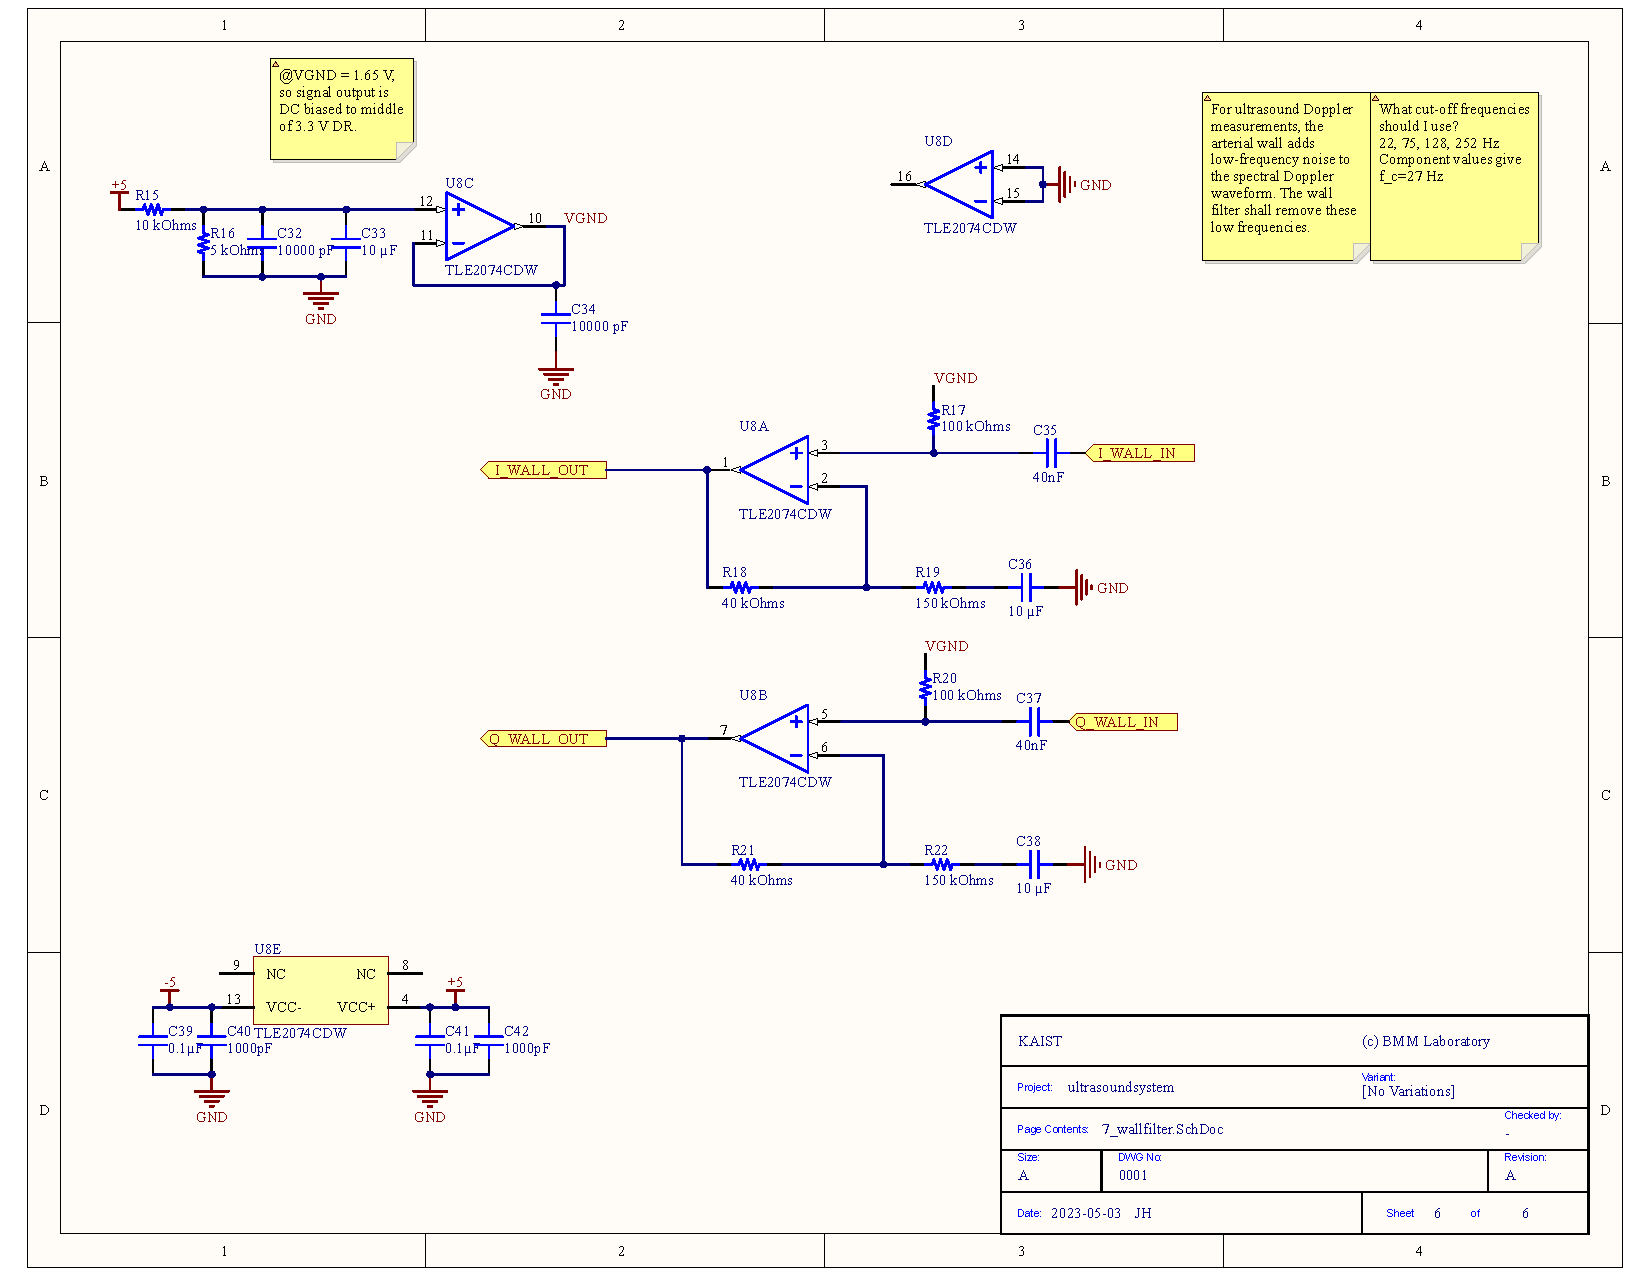
\includegraphics[width=20cm,height=28.7cm,keepaspectratio]{Figures/appendix/afe_altium/7_wallfilter.pdf}
		\caption{AFE Wall Filter}
		\label{fig:appendix_7_wallfilter}
	\end{figure}
\end{landscape}
\begin{landscape}
	\begin{figure}[htbp]
		\centering
		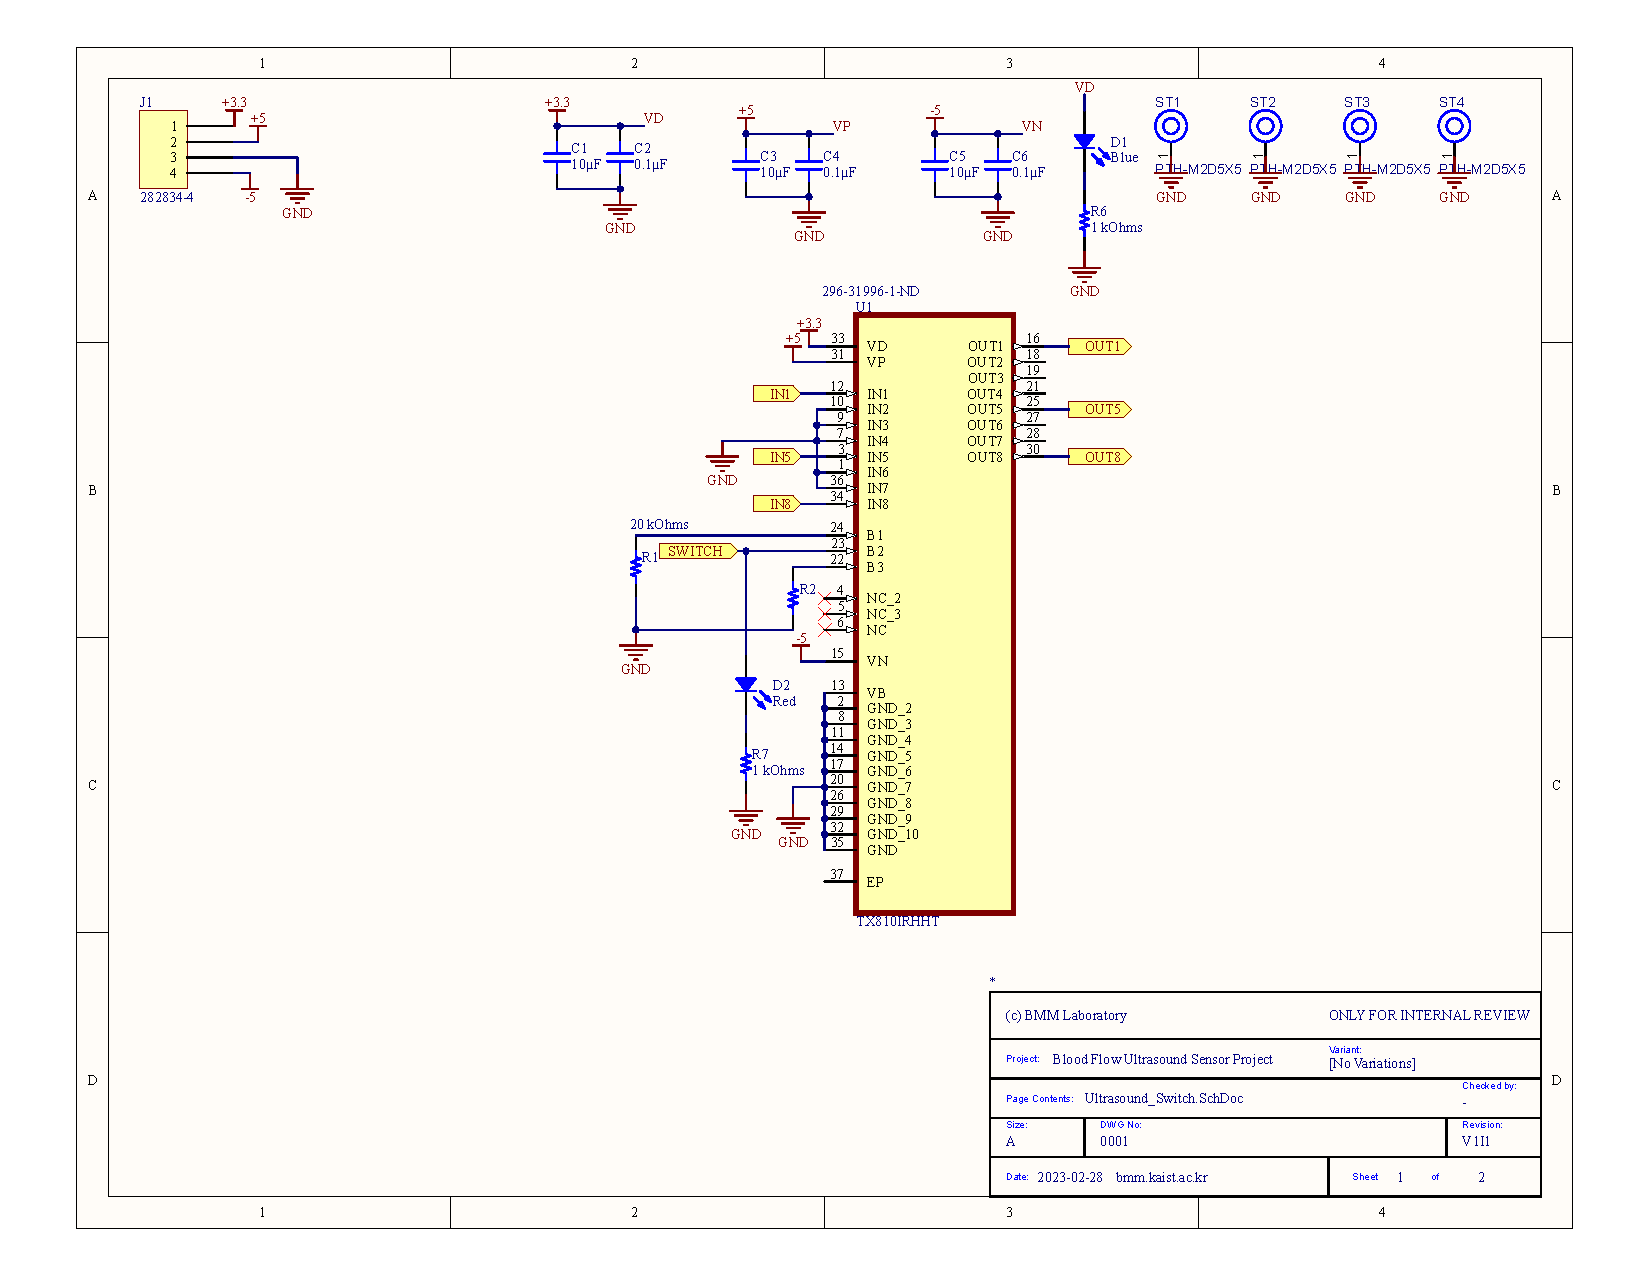
\includegraphics[width=20cm,height=28.7cm,keepaspectratio]{Figures/appendix/ultrasound_switch.pdf}
		\caption{UltrasoundSwitch Schematic A}
		\label{fig:appendix_ultrasoundswitch_a}
	\end{figure}
\end{landscape}
\begin{landscape}
	\begin{figure}[htbp]
		\centering
		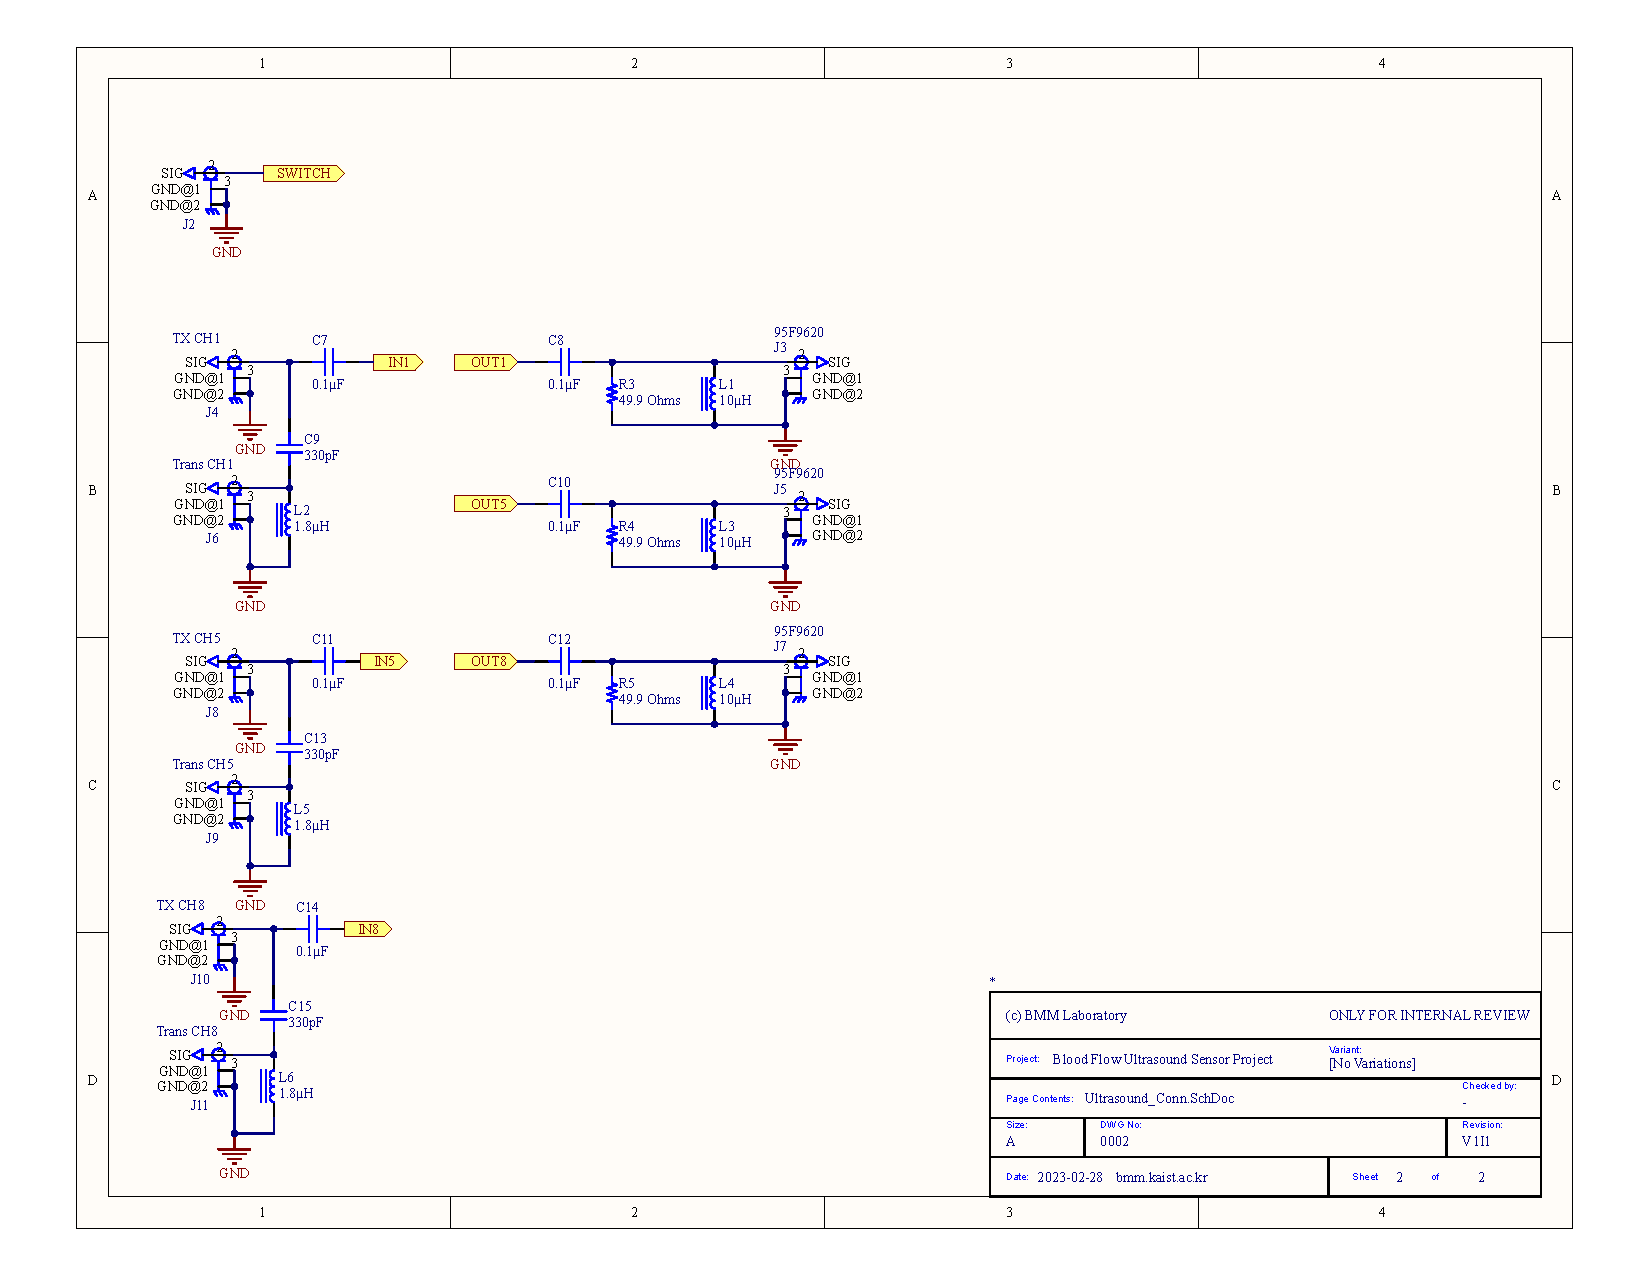
\includegraphics[width=20cm,height=28.7cm,keepaspectratio]{Figures/appendix/ultrasound_conn.pdf}
		\caption{UltrasoundSwitch Schematic B}
		\label{fig:appendix_ultrasoundswitch_b}
	\end{figure}
\end{landscape}
\begin{landscape}
	\begin{figure}[htbp]
		\centering
		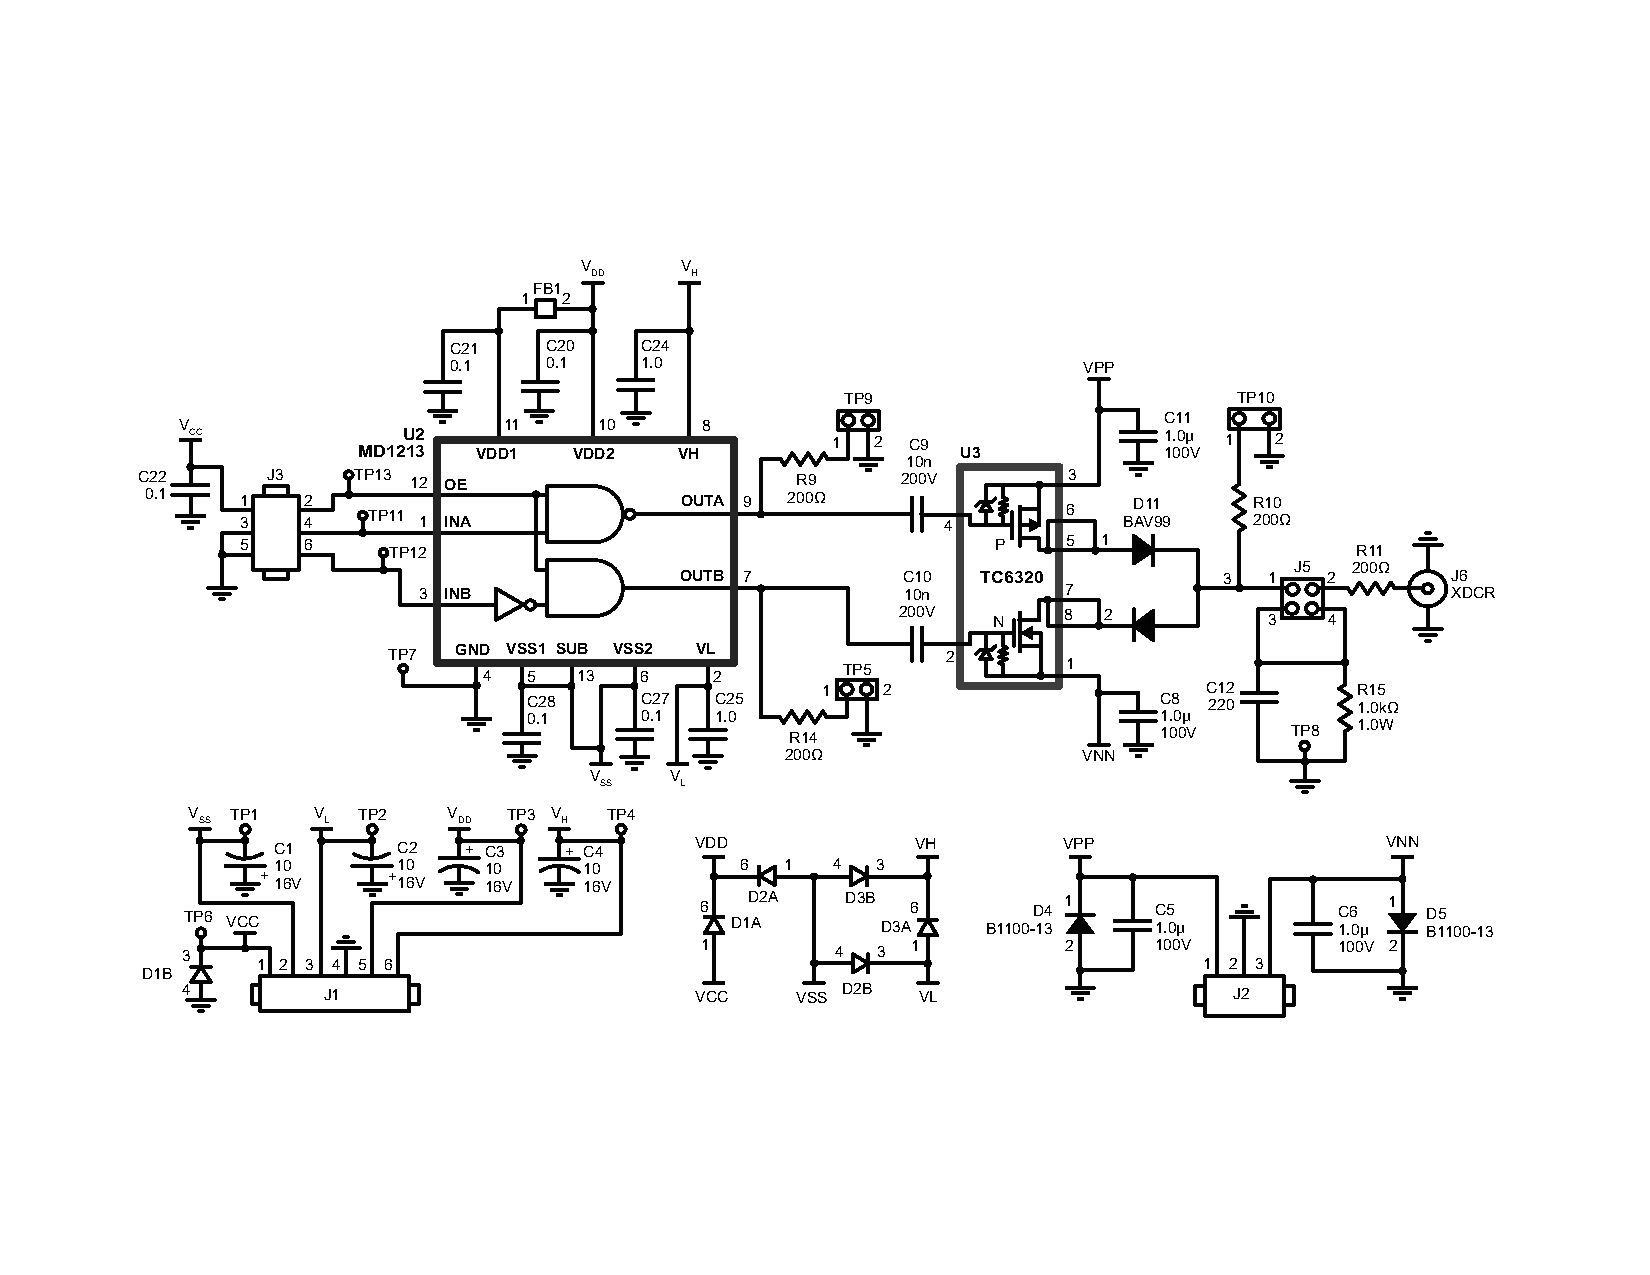
\includegraphics[width=20cm,height=28.7cm,keepaspectratio]{Figures/appendix/md1213db1_final.pdf}
		\caption{MD1213DB1 Transmitter Schematic}
		\label{fig:appendix_md1213db1}
	\end{figure}
\end{landscape}
\begin{landscape}
	\begin{figure}[htbp]
		\centering
		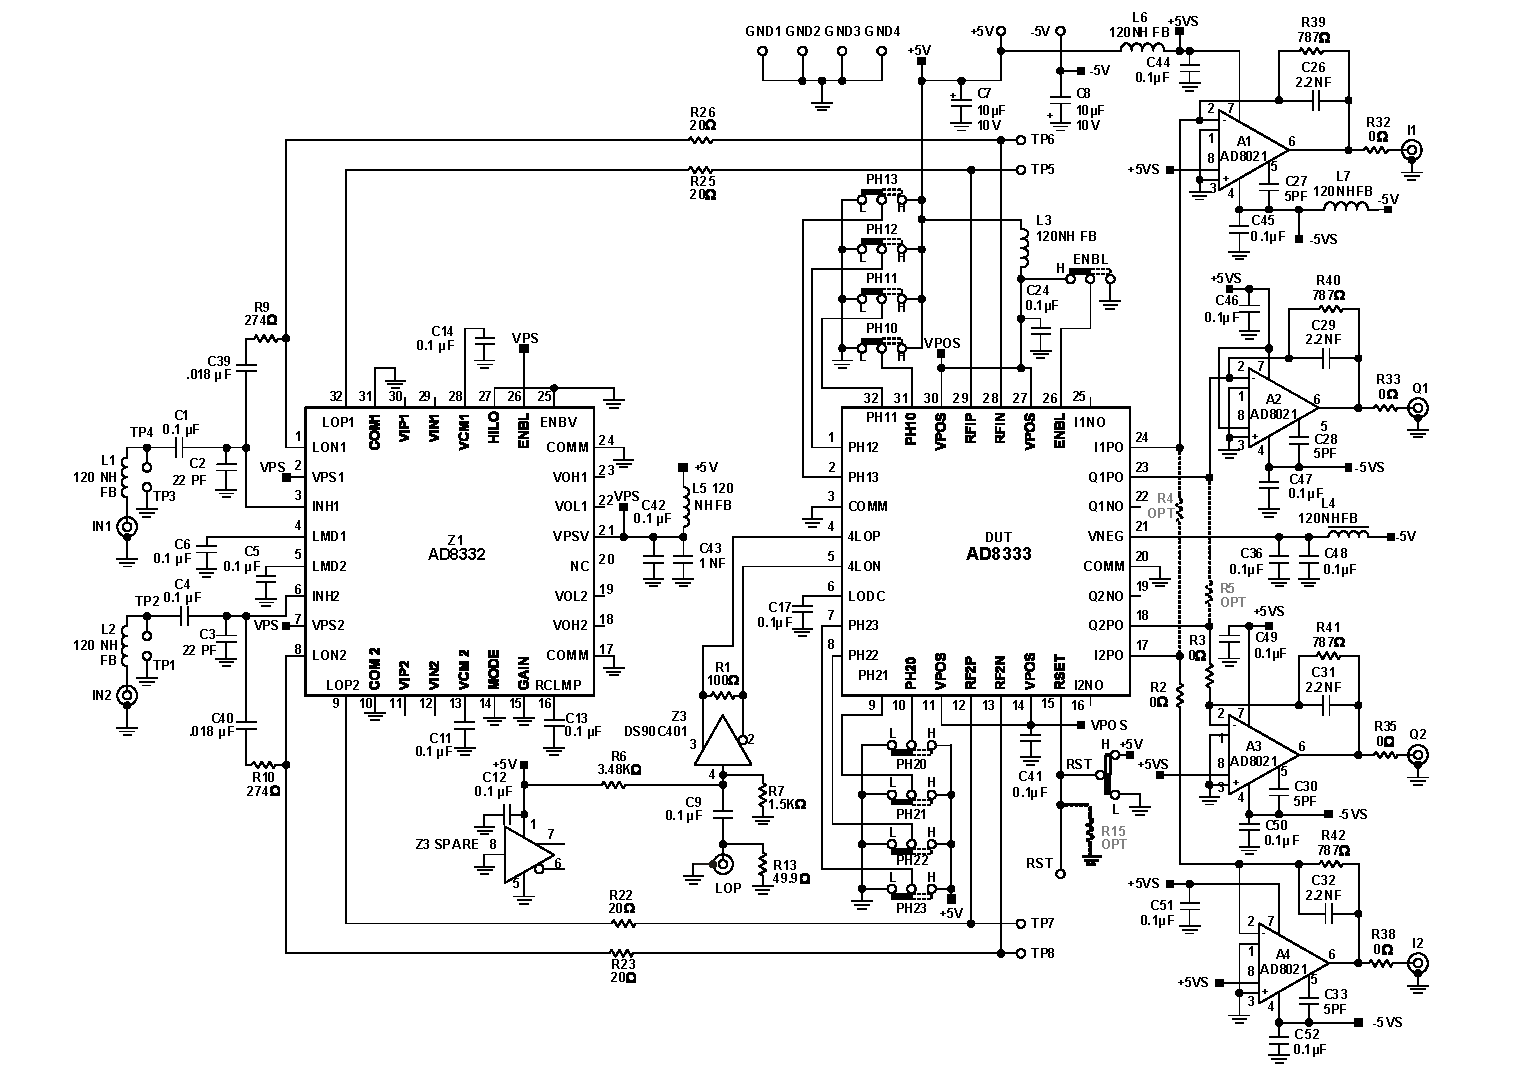
\includegraphics[width=20cm,height=28.7cm,keepaspectratio]{Figures/appendix/ad8333evalz.pdf}
		\caption{AD8332 Preamplifier, AD8333 IQ Demodulator Schematic}
		\label{fig:appendix_ad8333}
	\end{figure}
\end{landscape}
\chapter{Circuit CAD Assembly Documentation}
\begin{landscape}
	\begin{figure}[htbp]
		\centering
		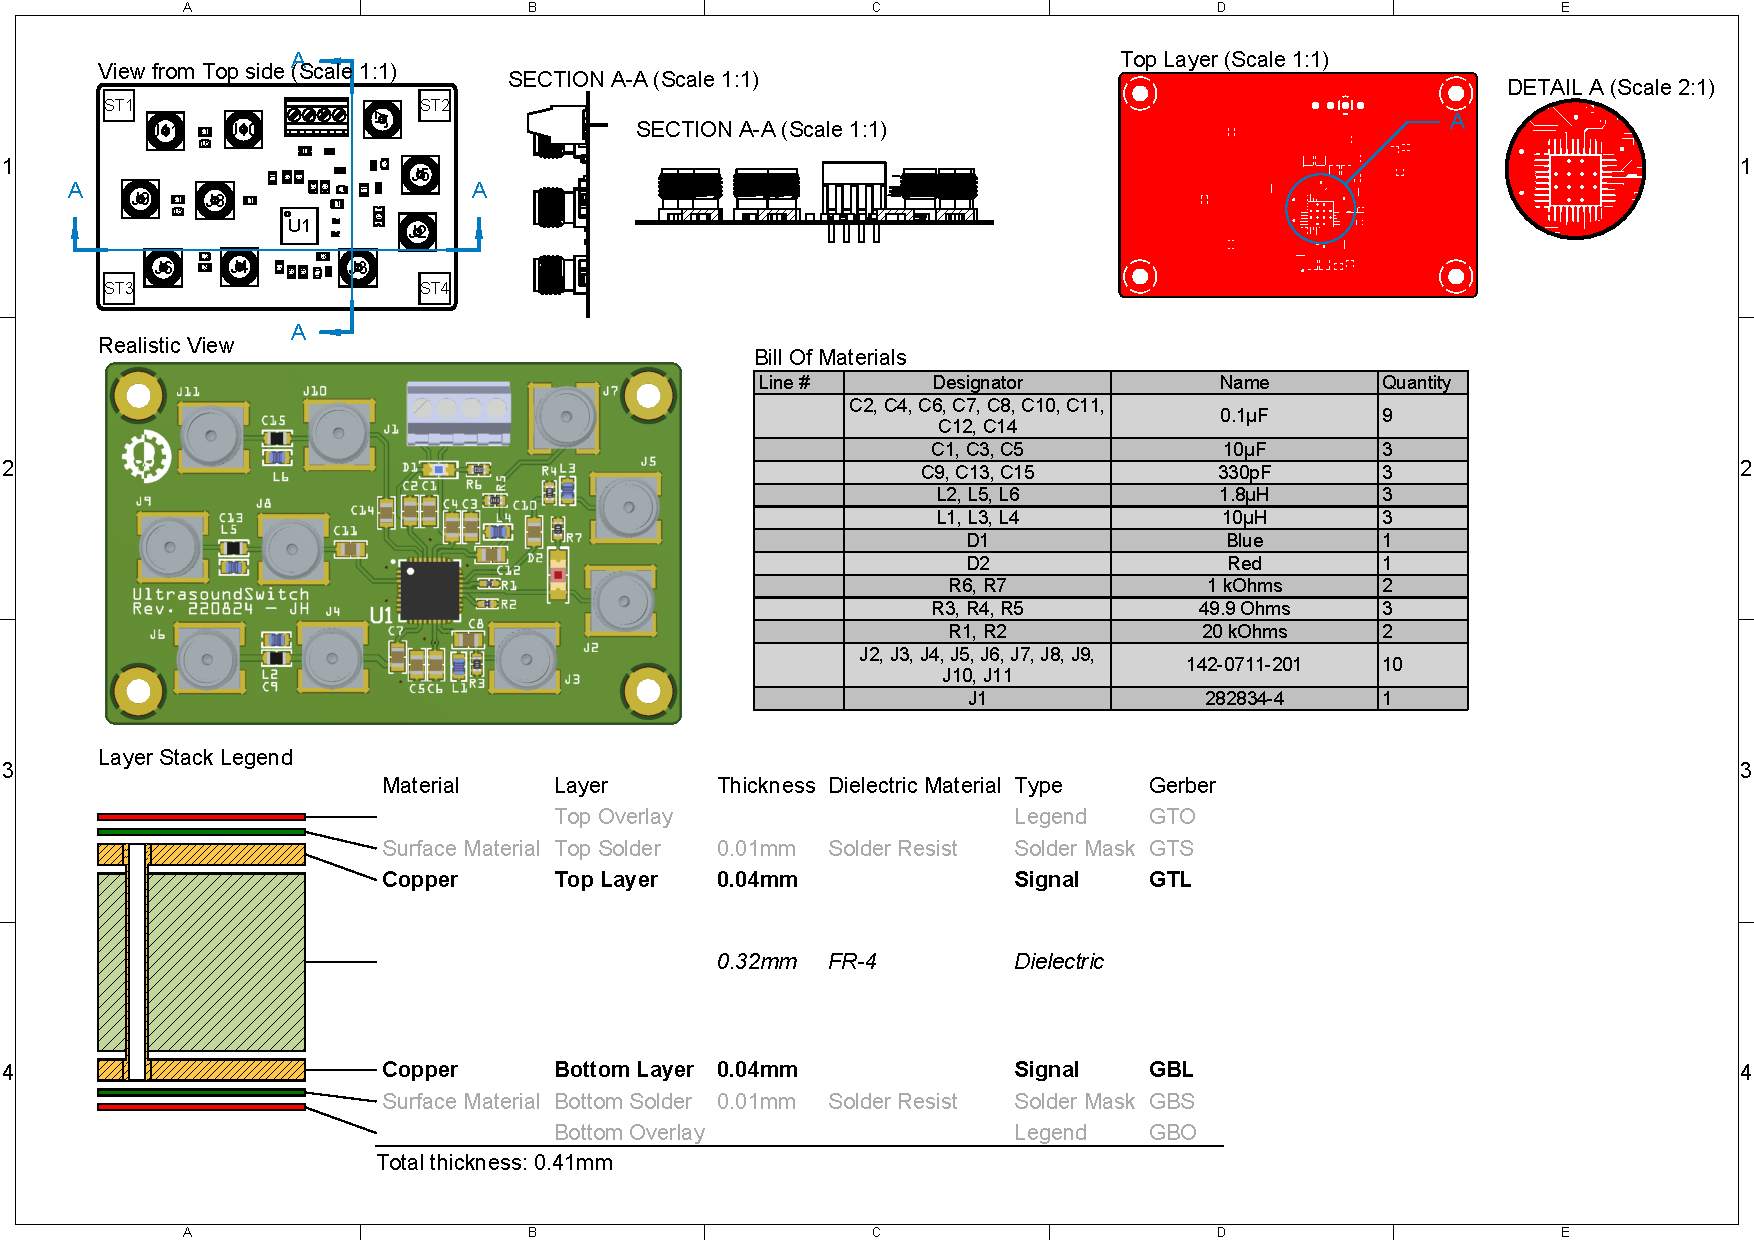
\includegraphics[width=20cm,height=28.7cm,keepaspectratio]{Figures/appendix/draftsman.pdf}
		\caption{UltrasoundSwitch Assembly Information}
		\label{fig:appendix_ultrasoundswitch_assembly}
	\end{figure}
\end{landscape}

%\chapter{Bill of Materials} \thispagestyle{main}
%
%	\begin{longtblr}[
%		%	theme=fancy,
%		caption = {Bill of Materials for the entire system},
%		entry={BOM},
%		label = {tab:bom}
%		]{
%			colspec = {lllll},
%			width = \linewidth,
%			rowhead = 1,
%%			hspan=minimal,
%			%vspan=minimal,
%		}
%		\toprule
%		{\textbf{Component}}
%		& {\textbf{Value}}
%		& {\textbf{Footprint}}
%		& {\textbf{Classification}}
%		& {\textbf{Description}}                              \\
%		\midrule
%		% table body
%		\SetCell[c=5]{c}{} Transmitter & & & & \\ \midrule
%		C1 & 1n & 0603 & X7R50V & Preamp \\
%		C13 & 1u & RAD-0.3in & Film 40V & Preamp \\
%		C14 & 1.5n & 0603 & X7R50V & PI controller \\
%		C15 & NC & 0603 & X7R50V & PI controller \\
%		C2,C3,C4 & 100n & 0603 & X7R16V & Decoupling \\
%		C5,C11 & 1u & 0603 & X5R6.3V & Decoupling \\
%		C6,C7 & 100n & 0805 & X7R50V & Decoupling \\
%		C8 & 1500u & RAD-0.3in & 63Vdc & Decoupling \\
%		P10 & 3-pin & Male & 250V & Controller bypass \\
%		P11,P12 & 10-pin & Female & 250V & InterPCB con. \\
%		P2,P3 & 1-pin header & Male & 250V & Measurements \\
%		P4,P5 & 2-way screw & NA & 300V 15A & Power,Output \\
%		P6 & 2-pin header & KK254 & 500V 4A & Audio in \\
%		P7 & 4-pin header & Female & 250V & 5V Power \\
%		P8,P9 & BNC & PCB & 500V & Audio in, Output \\
%		R2 & 16.2k & 0603 & 1\% & Preamp \\
%		R1,R3 & 2k & 0603 & 1\% & Preamp \\
%		R4,R7 & 4.75k & 0603 & 1\% & Voltage ref \\
%		R5 & 33.2k & 0603 & NA & PI controller \\
%		R6 & 0 (short) & 0603 & NA & PI controller \\
%		R9 & 0 (short) & 0603 & NA & PI controller \\
%		R10 & NC & 0603 & NA & PI controller \\
%		R8 & 2.49k & 0603 & 1\% & Voltage ref \\
%		U1 & OPA2365 & SOIC-8 & NA & Preamp, PI \\
%		U2 & TLV431A & SOT-23 & 1\% & Voltage ref \\ %\pagebreak
%		\SetCell[c=5]{c}{} Receiver & & & & \\ \midrule
%		C1,C11,C15 & 100n & 0603 & X7R16V & Gate driver \\
%		P1,P2 & 10-pin header & Male & 250V & InterPCB con. \\
%		C2,C16 & 150n & 0603 & X5R10V & Gate driver \\
%		C3,C10 & 100p & 0603 & NPO50V & Decoupling \\
%		L1,L2 & 1.768u & Radial & NA & Output filter \\
%		U1,U3 & LM5113 & WSON-10 & NA & Gate driver \\
%		R20 & 15m sense & 1210 & 1\% 1W & Output filter \\
%		R1,R6 & 500 & 3213 & NA & Gate driver \\
%		Q1,Q2,Q3,Q4 & BSZ097-N10NS5 & TSDSON-8 & NA & Power stage \\
%		R2,R5,R8,R10 & 5 & 0603 & 1\% & Gate driver \\
%		R4,R9 & 0 & 0603 & 1\% & Gate driver \\
%		D1,D2 & Diode & NA & 85V 0.25A & Gate driver \\
%		C5,C6,C9,C17 & 10u & 1210 & X7R50V & Decoupling \\
%		C12,C13,C14 & 680n & 1210 & X7R100V & Output filter \\
%		\SetCell[c=5]{c}{} Microcontroller & & & & \\ \midrule
%		C18,C20,C27 & 100n & 0603 & X7R16V & Decoupling \\
%		C28,C29 & 100n & 0603 & X7R16V & Decoupling \\
%		U6 & LT1999 & MSOP-8 & NA & Current acq. \\
%		U4 & AD8274 & MSOP-8 & NA & Volt acq. \\
%		U2 & LT1711 & MSOP-8 & NA & AIM \\
%		C4 & NC & 0603 & X7R16V & AIM \\
%		C7 & NC & 0603 & X7R16V & AIM \\
%		C8 & NC & 0603 & X7R16V & Cur. acq. \\
%		CA1 & 1.5n & 0603 & X7R50V & AIM \\
%		R14 & 8.66k & 0603 & 1\% & AIM \\
%		R18 & 16.2k & 0603 & 1\% & AIM \\
%		R23 & 1.5k & 0603 & 1\% & AIM \\
%		R3,R11 & 120k & 0603 & 1\% & Voltage acq. \\
%		RA1 & 2.2k & 0603 & 1\% & AIM \\
%		RA2 & 20k & 0603 & 1\% & AIM \\
%		RA3 & 2.74k & 0603 & 1\% & AIM \\
%		RA4 & 0 & 0603 & NA & AIM \\
%		\bottomrule
%	\end{longtblr}

\chapter{Instruments} \thispagestyle{main}
\begin{table}[ht]
	\centering
	\caption{List of instruments used for solder work}
	\label{tab:instruments_solder_work}
	\begin{tblr}[]{%
			colspec = {lll},
			row{1} = {guard, m, font=\small\bfseries},
		}
		\toprule
		Function & Manufacturer & Model \\ \midrule
		Visual inspection microscope & Leica & A60 \\
		Manual soldering & Weller & WX2 \\
		Heat gun & Thermaltronics & TMT-HA600-2 \\
		Solder paste & Chip Quik & SMD291AX250T3 \\
		Solder flux & Chip Quik & SMD291NL \\
		Reflow oven & Puhui & T-962A \\
		DMM & Fluke & 175 \\ \bottomrule
	\end{tblr}
\end{table}

\begin{table}[ht]
	\centering
	\caption{List of instruments used in experiments}
	\label{tab:instruments_hardware}
	\begin{tblr}[]{%
			colspec = {lll},
			row{1} = {guard, m, font=\small\bfseries},
		}
		\toprule
		Function & Manufacturer & Model \\
		\midrule
		DCPS 1 & RIGOL & DP832A 200W \\
		DCPS 2 & Keysight & E3631A 80W \\
		Function generator 1 & Keysight & 33500B \\
		Function generator 2 & Tektronix & AFG3102 \\
        DMM & Fluke & 175 \\
		Transducer (PZT) & HAGISONIC & M715-SB-S 204 \qty{5}{\mega\hertz} \\
		Transducer (CMUT) & BMM Creation & 6ch \qty{3.3}{\mega\hertz} C.F. \\
		RF Amplifier & Tomco & BT00100-AlphaS-CW \\
		Oscilloscope 1 & Keysight & DSO-X 2024A \\
		Oscilloscope 2 & Tektronix & MSO4054 \\
		Physiological simulator & CIRS & Doppler String Phantom 043A \\
		Vector Network Analyzer & Agilent & E5071B ENA Series Network Analyzer \\
		\bottomrule
	\end{tblr}
\end{table}

%\chapter{Embedded}
%\subsection{Zephyr}
%Zephyr is an \gls{open-source} \gls{rtos} designed to be lightweight and run on a wide range of devices, from \gls{mcu}s with as little as \qty{20}{\kilo\byte} of \gls{ram} to more powerful systems with multiple processors. Zephyr is designed to be modular and scalable, with a focus on security and low power consumption. It includes support for a wide range of hardware architectures, including ARM Cortex-M, x86, and RISC-V, and it can be used with a variety of development boards and microcontrollers. One of the key features of Zephyr is its ability to run on very small devices with limited resources. It includes support for various networking protocols, such as \gls{ble}, IPv4, and IPv6, which makes it well-suited for use in \gls{iot} applications. Zephyr is developed as part of the Linux Foundation's Zephyr Project, and it is widely used in the development of IoT and embedded systems.
%
%\subsubsection{Build System}
%To build an application with the Zephyr kernel, you use CMake which has two phases - configuration and build. During configuration phase, CMake executes the \texttt{CMakeLists.txt} build scripts to generate an internal model of the Zephyr build. Starting with \gls{dts} and \gls{dtsi} and then using the device-tree nodes and Kconfig to configure the set of build files for ninja.
%\begin{figure}[htbp]
%	\centering
%	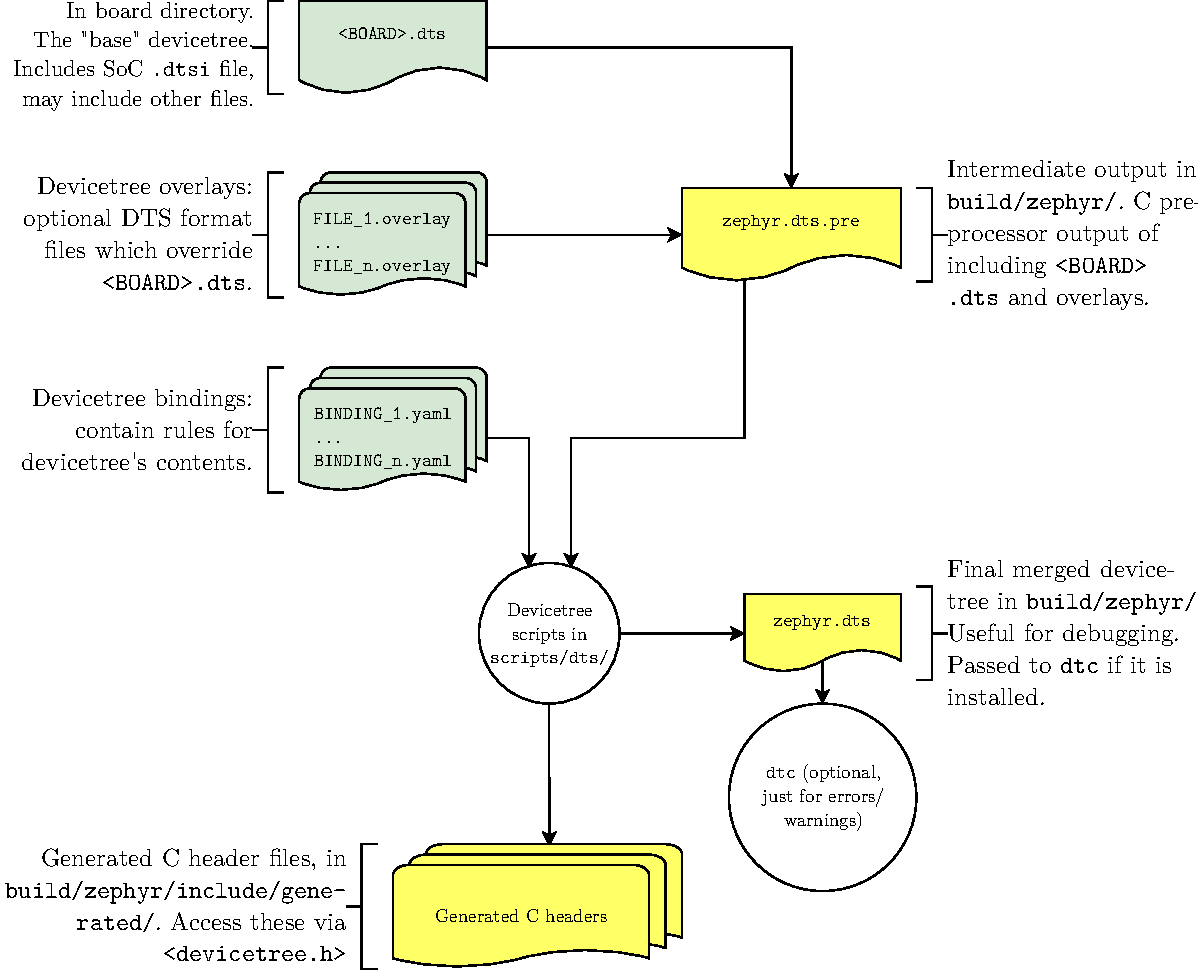
\includegraphics[width=.8\textwidth]{Figures/3_devicetree.pdf}
%	\caption[Devicetree input files and output files]{Devicetree input files (green) and output files (yellow) \cite{zephyrprojectdocumentation}}
%	\label{fig:3_devicetree}
%\end{figure}
%Seen in \cref{fig:3_devicetree} is the process in which the build system searches out device-trees in certain locations and merges them into the \texttt{zephyr.dts} that will be used for configuring and mapping every peripheral. Typically, each supported board has a file called \texttt{BOARD.dts} that defines the hardware of the board. The \texttt{BOARD.dts} file includes one or more \texttt{.dtsi} files that describe the CPU or system-on-chip that Zephyr runs on, and other common hardware features shared by multiple boards. These \texttt{.dtsi} files may also include other \texttt{.dtsi} files. Additionally, the \texttt{BOARD.dts} file provides a description of the specific hardware of the board. After parsing the \texttt{BOARD.dts} file, the main point being the merge with the \texttt{.overlay} file specific to both the project and the board. This overlay enables the portability feature of Zephyr. A significant degree of the workload when implementing Zephyr projects are thus in writing hardware devicetrees and then writing as generic firmware implementations as possible. Next, the configuration phase can be seen in \cref{fig:3_cmake_configuration}. Once configuration phase is done, CMake generates build scripts that are native to the host platform and initiate the build sequence with the build system Ninja \cite{ninja}. Afterwards, the generated build scripts are executed to begin the second phase, build. The build scripts can recompile the application without involving CMake after most code changes. Zephyr uses the \enquote{target} concept of CMake to organize the build, where a target can be an executable, a library, or a generated file. The final output of Ninja is a binary file ready for \gls{flashing} using a microcontroller programmer.
%
%\begin{figure}[htbp!]
%	\centering
%	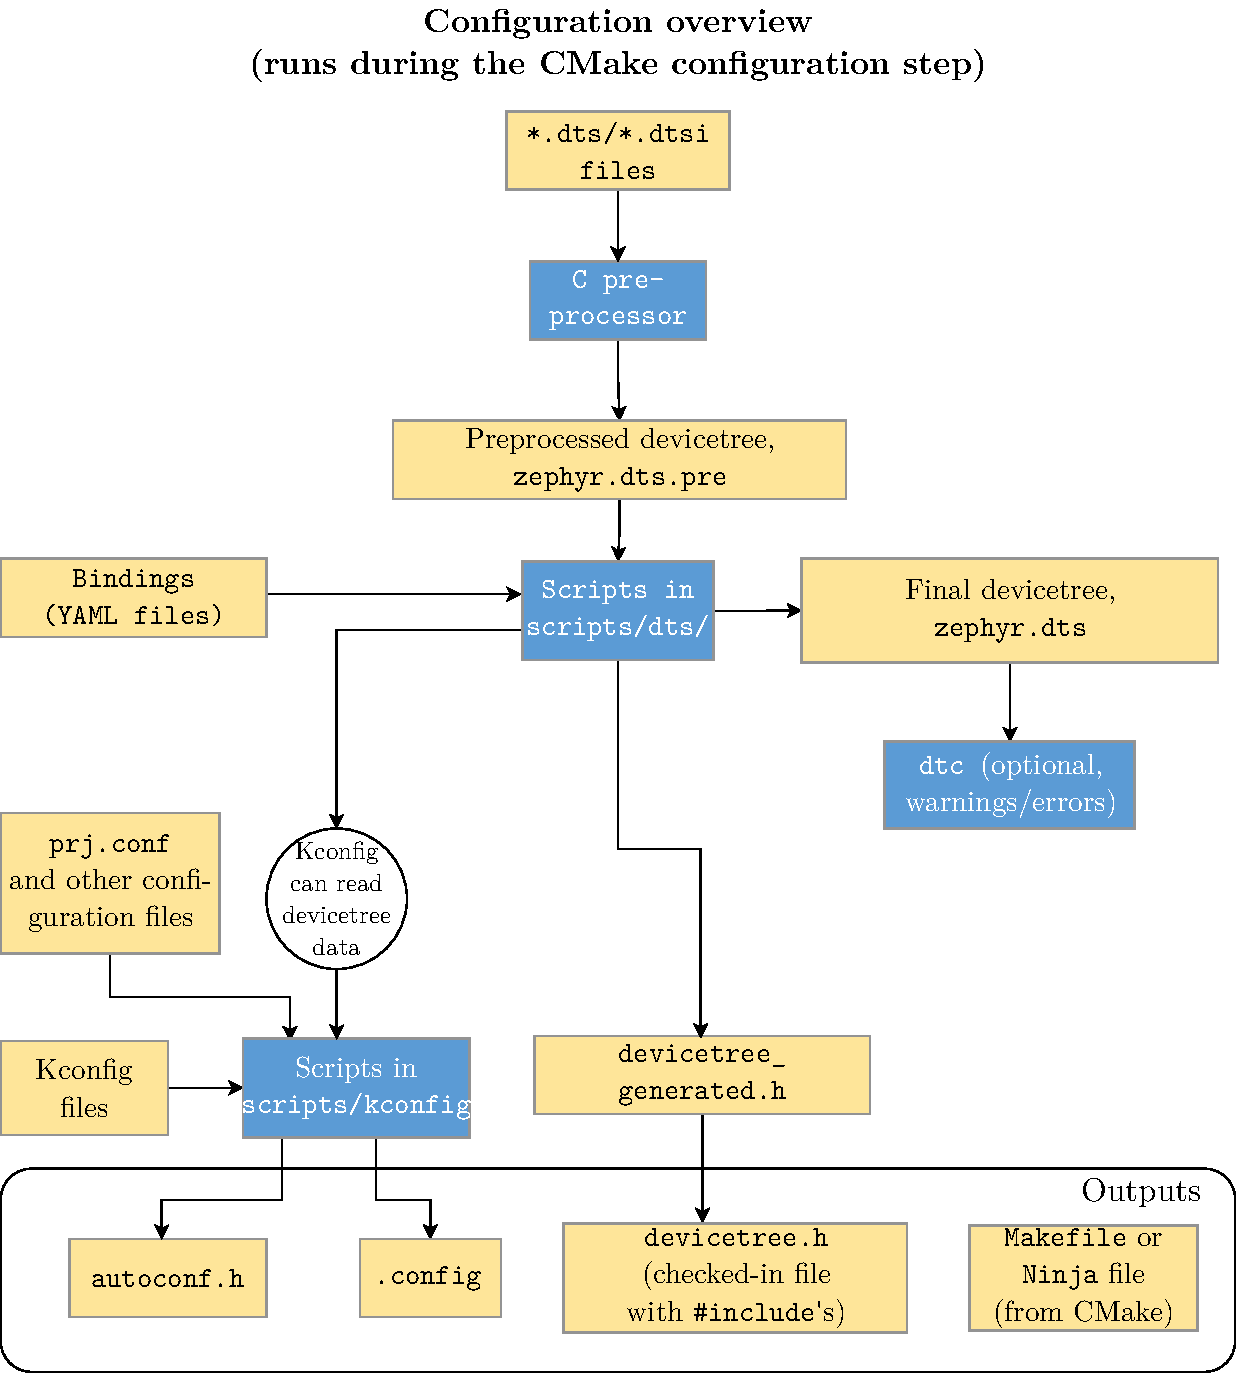
\includegraphics[width=.8\textwidth]{Figures/3_cmake_configuration.pdf}
%	\caption[Configuration phase of a Zephyr application]{Configuration phase of a Zephyr application \cite{zephyrprojectdocumentation}}
%	\label{fig:3_cmake_configuration}
%\end{figure}
%After cmake configuration phase has completed, the build phase begins. CMake invokes the build system, which (conceptually) has five (six, one is repeated) stages: (I) pre-build, (II) generation and compilation, (III) first-pass binary (and (IV) second-pass binary), (V) final binary and (VI) post-processing.
%\begin{figure}[htbp]
%	\centering
%	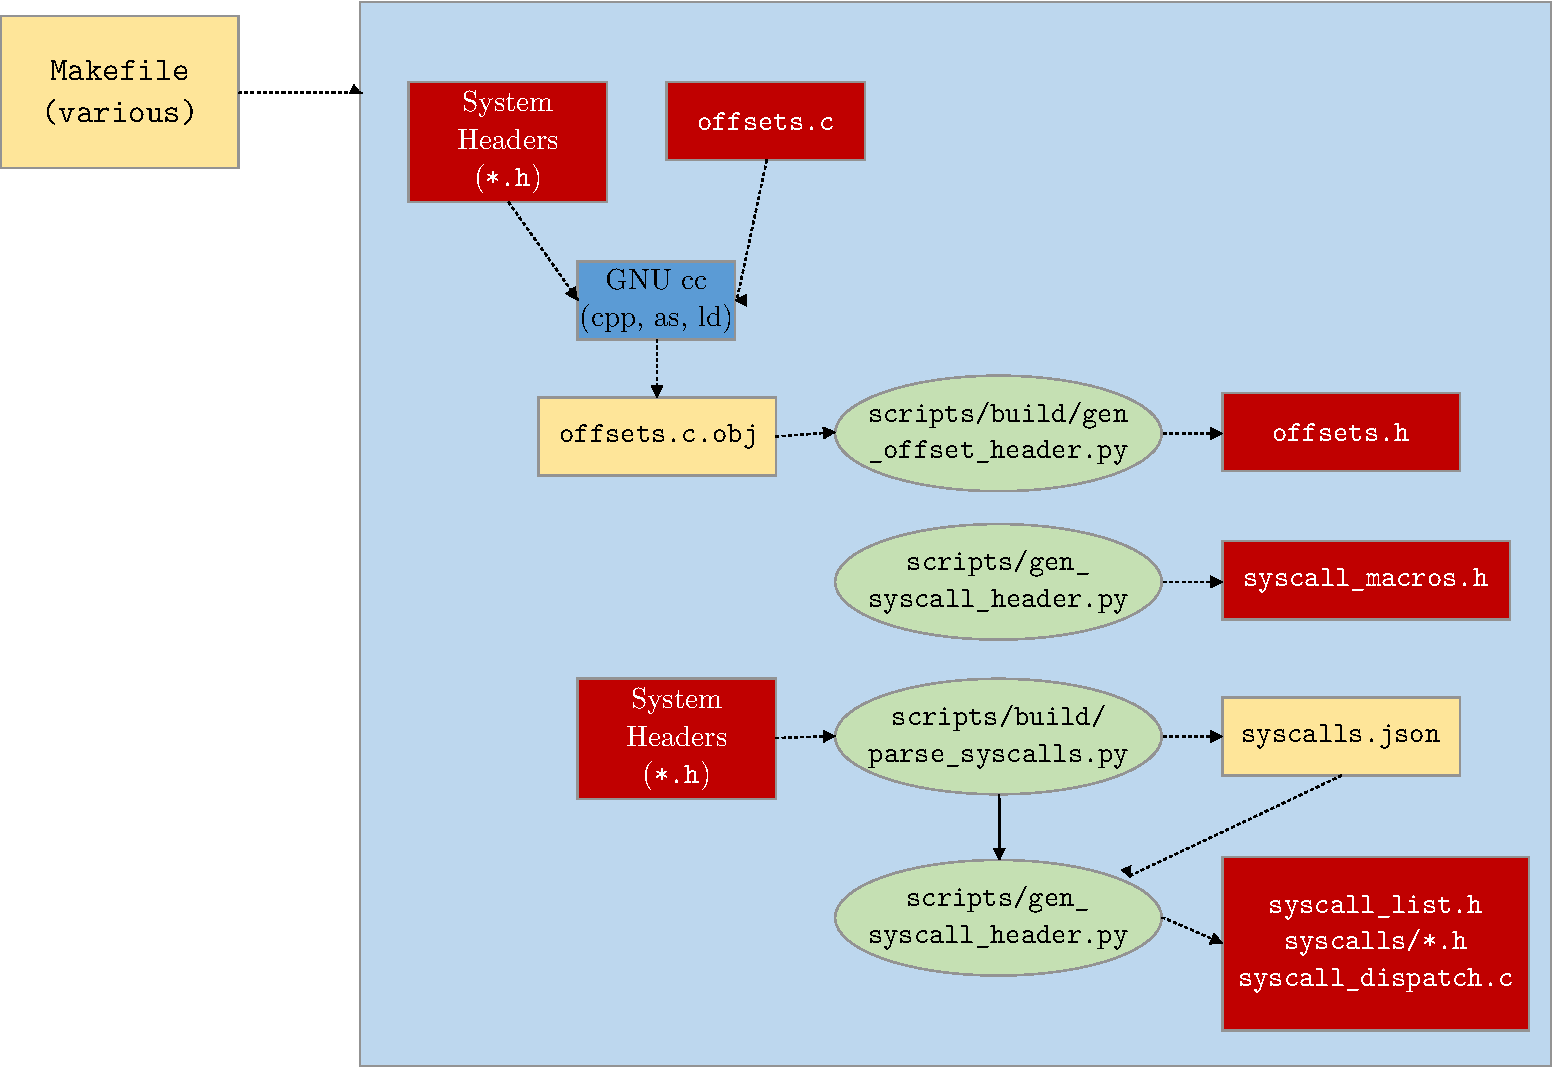
\includegraphics[width=.8\textwidth]{Figures/3_cmake_build1.pdf}
%	\caption[Flowchart of build stage I, pre-build]{Flowchart of build stage I, pre-build}
%	\label{fig:3_build1}
%\end{figure}
%In \cref{fig:3_build1} the build system binds system call functions to implementations.
%\begin{figure}[htbp]
%	\centering
%	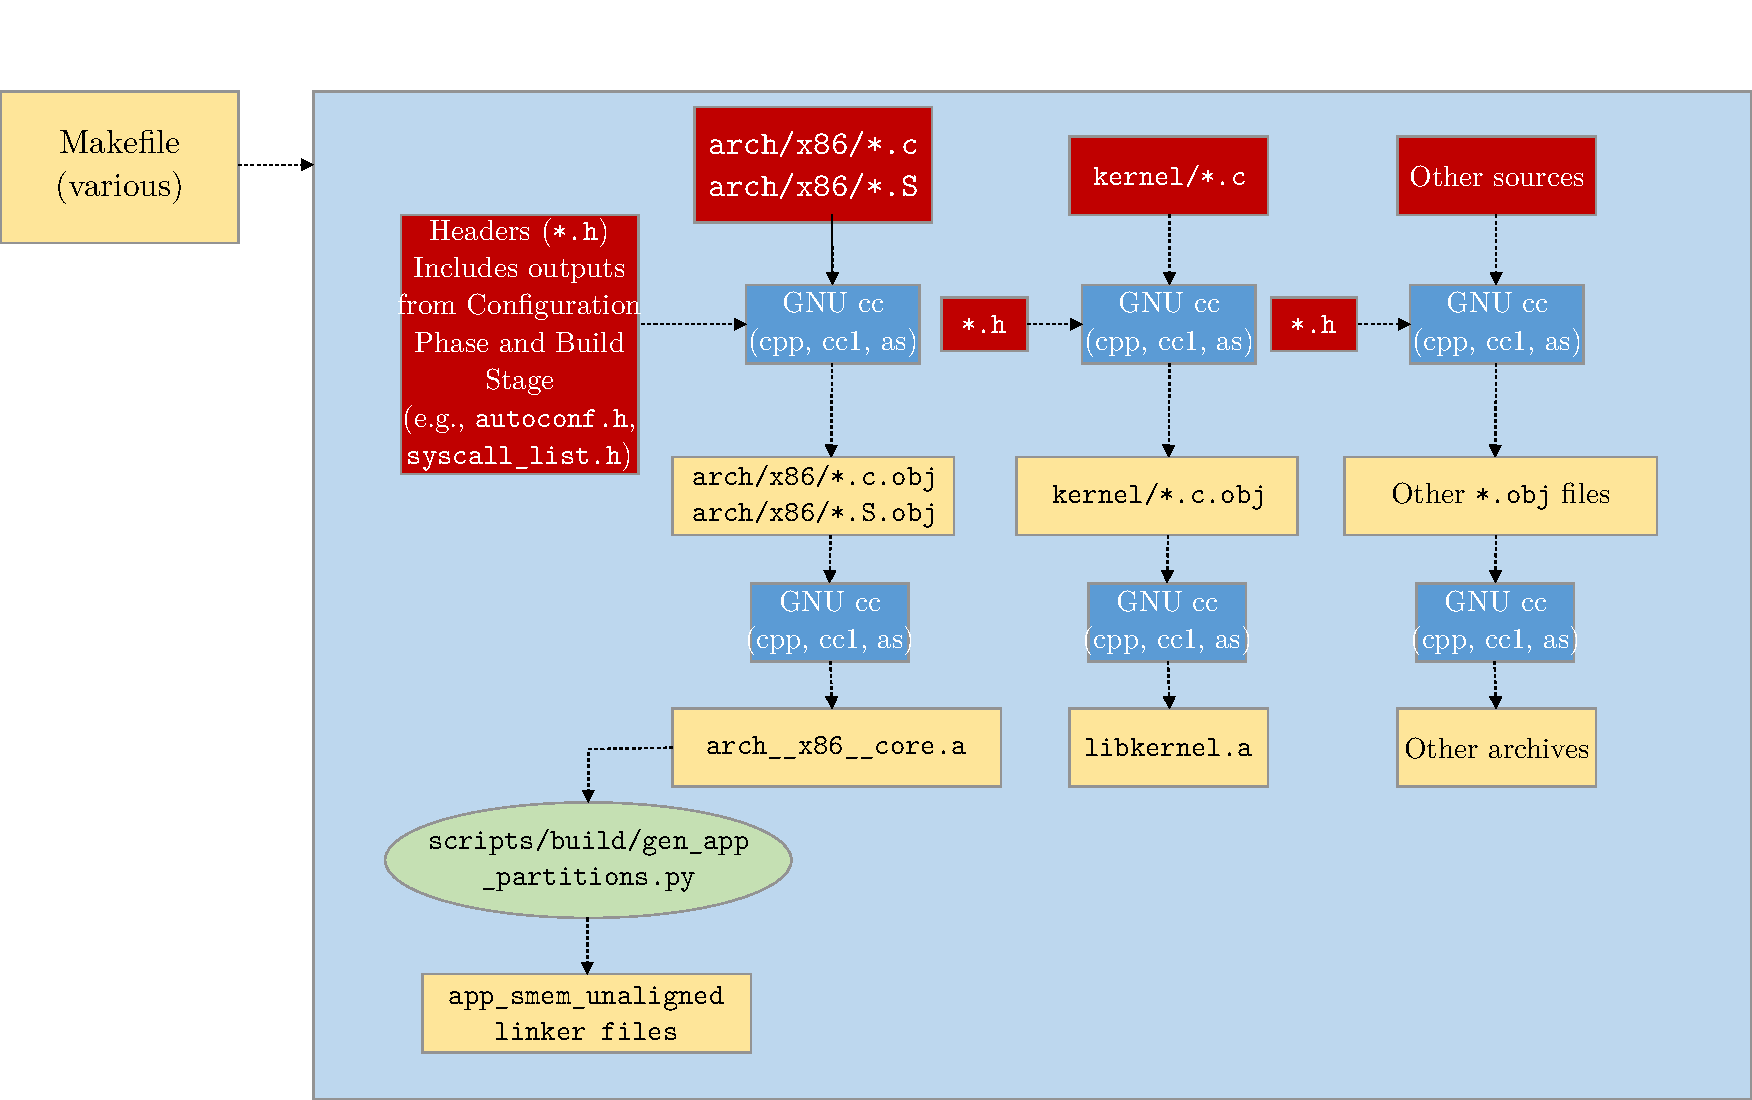
\includegraphics[width=.8\textwidth]{Figures/3_cmake_build2.pdf}
%	\caption[Flowchart of build stage II, generation and compilation]{Flowchart of build stage II, generation and compilation}
%	\label{fig:3_build2}
%\end{figure}
%Next, in \cref{fig:3_build2} the build system collects source files for various subsystems (decided by the configuration phase) and compiles into archives. The \texttt{gen\_app\_partitions.py} script examines all the archives that are produced and creates linker scripts that organize and align application partitions correctly, based on the memory protection hardware of the target. Then \texttt{cpp} process involves merging linker script fragments from various sources, including the target's architecture/\gls{soc}, the kernel tree, partition output (if memory protection is enabled), and any other selected fragments from the configuration process. These are combined into a \texttt{linker.cmd} file. The compiled archives are then linked with \texttt{ld}, following the specifications in the \texttt{linker.cmd} file.
%\begin{figure}[htbp]
%	\centering
%	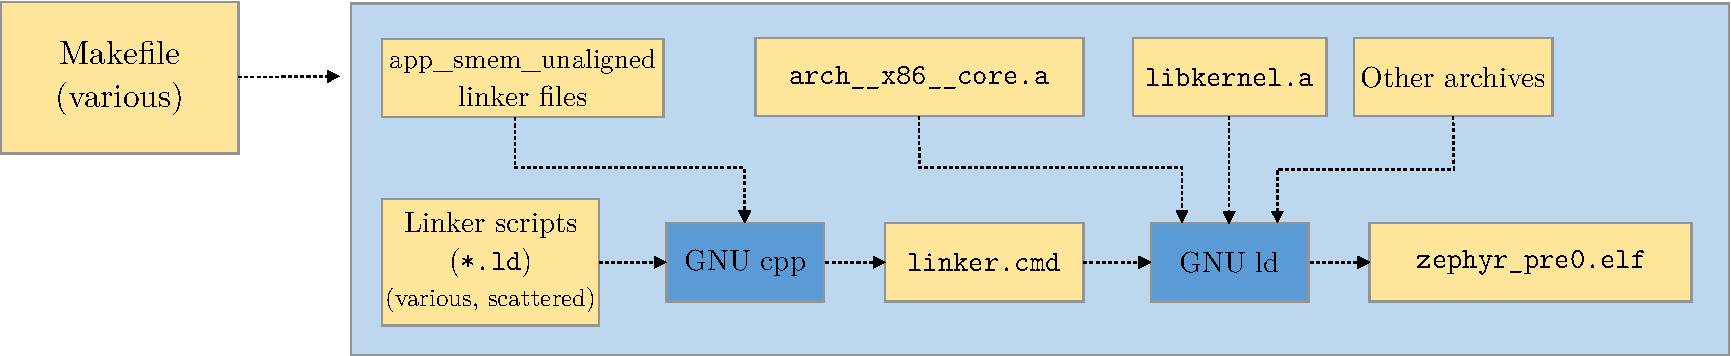
\includegraphics[width=.8\textwidth]{Figures/3_cmake_build3.pdf}
%	\caption[Flowchart of build stage III, intermediate binary]{Flowchart of build stage III, intermediate binary}
%	\label{fig:3_build3}
%\end{figure}
%Shown in \cref{fig:3_build3} is the process, in which an unfixed size intermediate binary is produced. If a devicetree is being used, an intermediate binary is generated that has a variable size. The binary is not fixed in size, which means that it can be modified by post-processing steps that affect the size of the final binary.
%\begin{figure}[htbp]
%	\centering
%	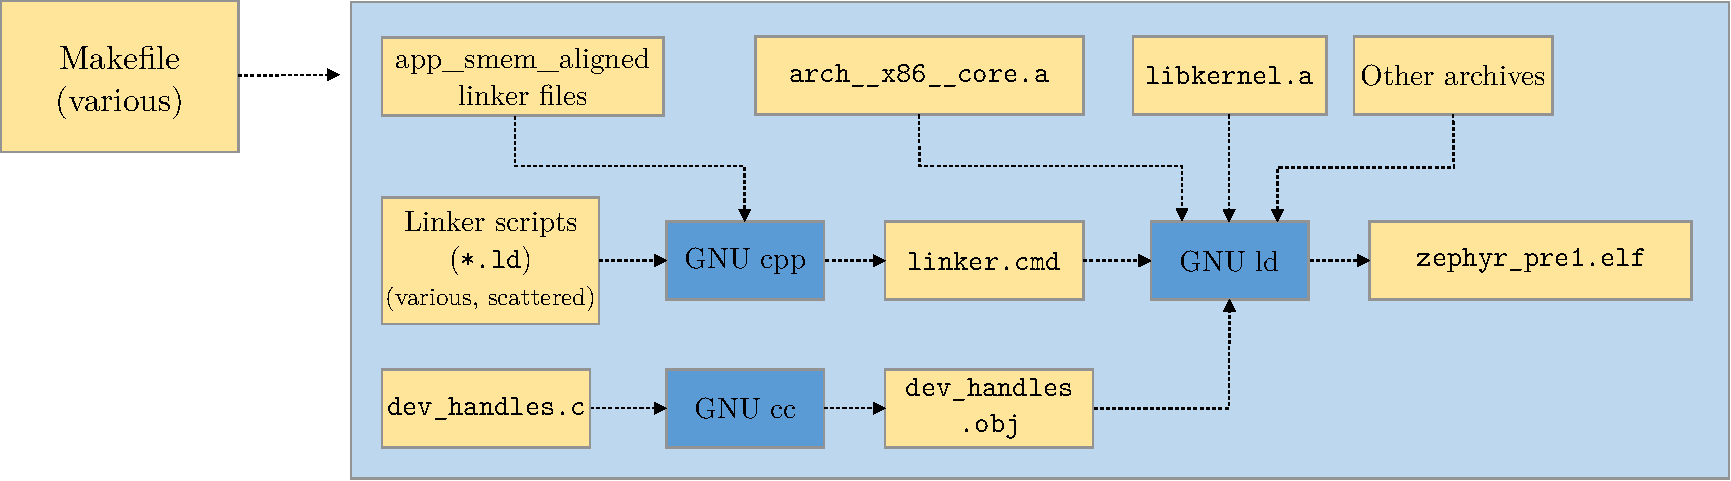
\includegraphics[width=.8\textwidth]{Figures/3_cmake_build4.pdf}
%	\caption[Flowchart of build stage IV, second intermediate binary]{Flowchart of build stage IV, second intermediate binary}
%	\label{fig:3_build4}
%\end{figure}
%In \Cref{fig:3_build4} the fixed size intermediate binary is generated. The previous stage's binaries are not fully formed and contain sections that are empty or marked as placeholders. These sections must be filled in by a process similar to reflection. To finish building, certain scripts are run on the intermediate binaries. These scripts generate the necessary components that are missing from the final binary.
%\begin{figure}[htbp]
%	\centering
%	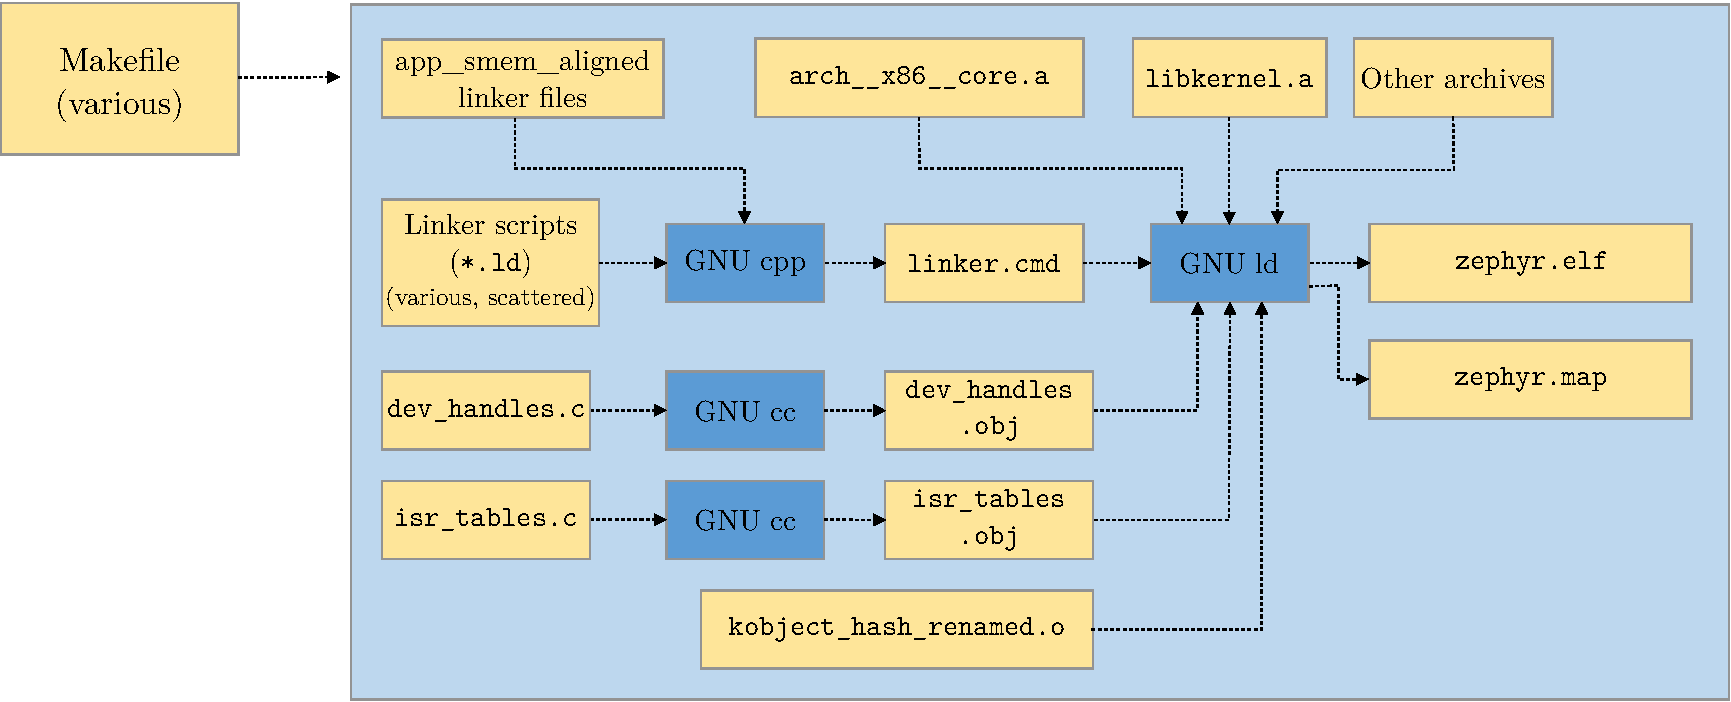
\includegraphics[width=.8\textwidth]{Figures/3_cmake_build5.pdf}
%	\caption[Flowchart of build stage V, final binary]{Flowchart of build stage V, final binary}
%	\label{fig:3_build5}
%\end{figure}
%Next, in \cref{fig:3_build5}, the final binary is produced by repeating the link from the previous stage, but this time with all the missing pieces populated.
%\begin{figure}[htbp]
%	\centering
%	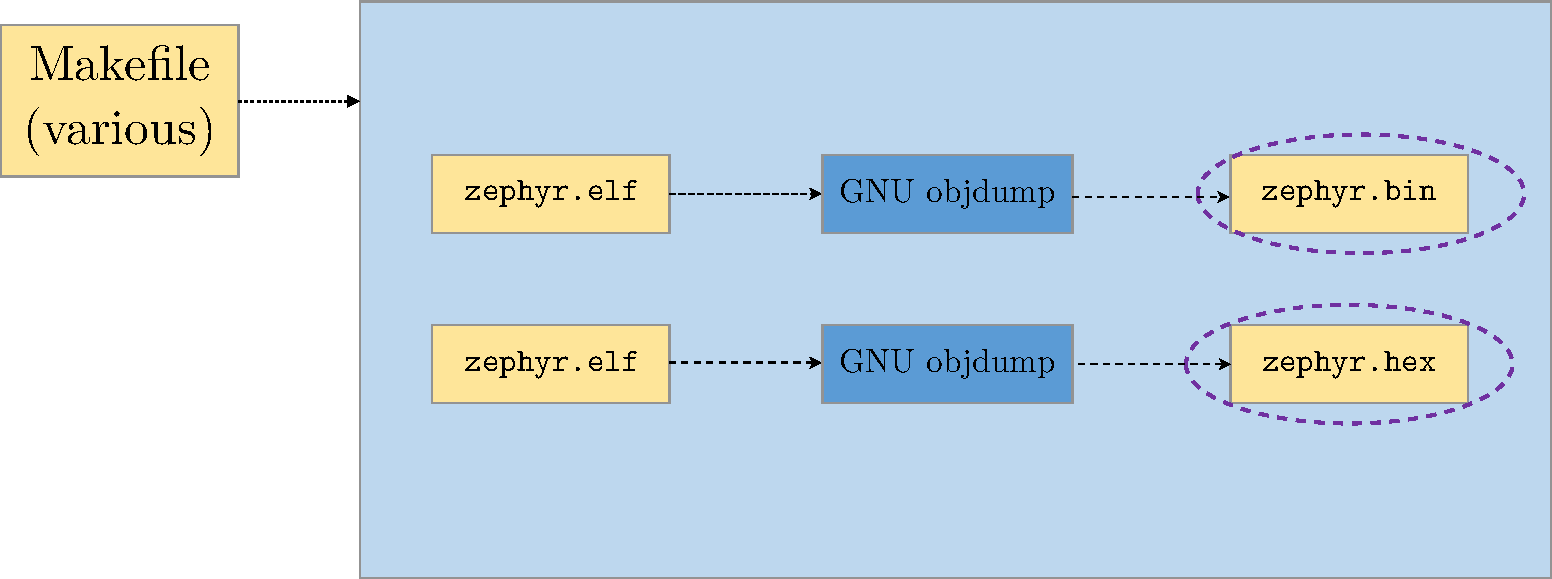
\includegraphics[width=.6\textwidth]{Figures/3_cmake_build6.pdf}
%	\caption[Flowchart of build stage VI, post-processing]{Flowchart of build stage VI, post-processing}
%	\label{fig:3_build6}
%\end{figure}
%Finally, in \cref{fig:3_build6}, using \texttt{GNU objdump}, the completed kernel is converted from a \gls{elf} file to the hex file that is expected by the flash tool compatible with the target device.

%\subsection{Firmware}
%A full repository of the revision controlled codebase is available on GitHub at \cite{github_firmware}.
%\cleartoleftpage
%\newgeometry{left=28mm,right=14mm,top=42mm,bottom=14mm}
\thispagestyle{empty}
\pagecolor{frontbackcolor}
\color{white}

\blindtext % Remove this for a blank page or write your own text

\vspace*{\fill}



\begin{tabular*}{\textwidth}{l @{\extracolsep{\fill}} r}
    \textbf{\dtudepartment} & \textbf{\kaistdepartment} \\
    Technical University & Korea Advanced Institute\\ 
    of Denmark & of Science \& Technology\\ 
    & \\
    \dtuaddressI & \kaistaddressI \\
    \dtuaddressII & \kaistaddressII \\
    Tel. (+45) 4525 3800 & Tel. (+82) 042-350-2114 \\
    \\
    \url{\dtudepartmentwebsite} & \url{\kaistdepartmentwebsite}
\end{tabular*}


\end{document}